\documentclass[final,a4paper,openany,12pt]{mwbk}
%\documentclass[final,a4paper,openright,12pt]{mwbk} % każdy rozdział zaczyna się na stronie nieparzystej
\usepackage{polski}
\usepackage[utf8]{inputenc}
\usepackage{fancyhdr}
\usepackage{xurl}
\usepackage{algorithm}
\usepackage{algpseudocode}
\usepackage{float}
\usepackage{tikz}
\usepackage{hyperref}
\usepackage{wrapfig}
\usepackage{caption}
\captionsetup{width=0.55\textwidth}


\usepackage{makeidx}  % allows index generation
\usepackage{graphicx} % standard LaTeX graphics tool
                      % for including eps-figure files

% ustawienia do wydruku dwustronnego z uwzględnieniem dodatkowego miejsca na zszycie
\setlength{\oddsidemargin}{0.46cm}   %margines nieparzysty
\setlength{\evensidemargin}{-0.54cm} %margines parzysty
\setlength{\textwidth}{16cm}         %szerokość tekstu na stronie
\linespread{1.1}    % lekkie zwiększenie odstępu między liniami, żeby tekst nie był taki ścisły, ponieważ
                    % Odstęp pojedynczej interlinii nie jest komfortowy, kiedy trzeba czytać strony A4
% koniec ustawień


\def\checkmark{\tikz\fill[scale=0.4](0,.35) -- (.25,0) -- (1,.7) -- (.25,.15) -- cycle;} 

                      
\begin{document}

\begin{titlepage}
\vspace{-0.5cm}

{\centering
{\footnotesize
\begin{tabular}{c}
UNIWERSYTET KARDYNAŁA STEFANA WYSZYŃSKIEGO\\
W WARSZAWIE\\
\end{tabular}
}
\vspace{2.5cm}

{\footnotesize
\begin{tabular}{c}
WYDZIAŁ MATEMATYCZNO-PRZYRODNICZY\\
SZKOŁA NAUK ŚCISŁYCH\\
\end{tabular}
}
\vspace{3.5cm}

\renewcommand{\arraystretch}{1.5} % zwiększamy odległość między wierszami

{\normalsize
\begin{tabular}{c}
Filip Krawczyk\\
Nr alb.: 119230\\
Kierunek studiów: Informatyka\\
\end{tabular}
}

\vspace{1.5cm}

{\large
\begin{tabular}{c}
Aplikacja mobilna do zarządzania \\ 
biblioteką fiszek na system iOS \\
\end{tabular}
}

}

\renewcommand{\arraystretch}{1} % przywracamy domyślną odległość miedzy wierszami

\vspace{5cm}

\hspace{6cm}
\begin{tabular}{l}
Praca licencjacka\\
Promotor:\\
dr inż. Artur Mikitiuk
\end{tabular}

\vspace{3cm}

{\centering

{\small
\begin{tabular}{c}
{Warszawa, 2025}\\
\end{tabular}
}

}
\end{titlepage}



\tableofcontents
\listoffigures  

\sloppy

\chapter*{Wstęp}

\section*{Wprowadzenie}

W czasach rosnących wymagań edukacyjnych i zawodowych efektywne metody przyswajania wiedzy są kluczowym elementem rozwoju osobistego. Samodzielna nauka to obszerna dziedzina, oferująca różne techniki dostosowane do indywidualnych potrzeb uczących się osób. Jednym z jej najskuteczniejszych narzędzi, jest powtarzanie interwałowe.

Jest to metoda nauczania, wykorzystująca zaplanowane odstępy w czasie pomiędzy kolejnymi sesjami nauki, aby zwiększyć efektywność przenoszenia informacji do pamięci długotrwałej. Kluczowym elementem tej metody jest obserwacja, że ludzki umysł lepiej przyswaja i zapamiętuje informacje, gdy są one powtarzane w pewnych odstępach.

Najpopularniejszym sposobem powtarzania interwałowego jest używanie fiszek. Są to dwustronne karty, na których awersie jest napisane słowo lub pytanie, a na rewersie jego definicja lub odpowiedź. Podczas nauki użytkownik przegląda fiszki, próbując przypomnieć sobie informacje z rewersu, a następnie weryfikuje poprawność swojej odpowiedzi. Karty, których zawartość została poprawnie zapamiętana, są odkładane do powtórzenia w dalszej przyszłości, podczas gdy te, które sprawiają trudność, są powtarzane częściej.

\section*{Motywacja}

Wraz z rewolucją technologiczną wiele tradycyjnych narzędzi edukacyjnych przeszło do świata wirtualnego. Fiszki nie stanowią w tym wypadku wyjątku. Dzięki powszechnej dostępności smartfonów i innych urządzeń mobilnych, pojawiły się różne aplikacje oferujące wirtualne odpowiedniki papierowych kart do nauki, jednocześnie zawierające funkcjonalność niemożliwą do zaoferowania w ich analogowym odpowiedniku.

Mimo że istnieje wiele aplikacji do tworzenia fiszek w sklepie App Store, posiadają one wiele wad. Duża część z nich próbuje wymusić na użytkowniku kupno subskrypcji wersji premium, posiadają dużo reklam utrudniających korzystanie z aplikacji, albo ich zakup wymaga znacznego jednorazowego wydatku pieniężnego. Ponadto wiele z dostępnych rozwiązań charakteryzuje się nadmierną złożonością interfejsu, gdzie liczne funkcje i opcje zaciemniają podstawowy cel aplikacji.

\newpage
\section*{Cel pracy}

Głównym celem niniejszej pracy jest zaprojektowanie i implementacja minimalistycznej aplikacji do tworzenia oraz zarządzania katalogiem fiszek. Projekt koncentruje się na opracowaniu rozwiązania charakteryzującym się intuicyjnym, nieintruzywnym interfejsem użytkownika, który eliminuje zbędne elementy mogące zakłócać proces nauki. 

Aplikacja musi mieć możliwość zapełnienia tekstem przodu oraz tyłu fiszki. Dodatkowo w przypadku materiałów, które ciężko jest zapisać w postaci tekstu, jak na przykład wzory matematyczne, powinna dawać możliwość załączać zdjęcia. Częścią aplikacji powinien być także tryb nauki, w którym program wylosuje kolejność fiszek do nauki, oraz po nauce zapamięta, które z nich zostały oznaczone jako nienauczone i na podstawie tego będzie dostosowywać kolejność w następnych sesjach nauczania.

Z technicznego punktu widzenia, aplikacja zostanie zaprojektowana dla platformy iOS wykorzystaniem zintegrowanego środowiska programistycznego Xcode. Implementacja będzie oparta na języku Swift oraz bibliotece SwiftUI, co pozwoli na stworzenie responsywnego interfejsu użytkownika. Do zarządzania i przechowywania danych zostanie wykorzystana nowa biblioteka od Apple o nazwie SwiftData, zapewniająca efektywną warstwę persystencji dla informacji o fiszkach i postępach użytkownika.

\section*{Struktura pracy}

Praca składa się z pięciu rozdziałów. Pierwszy z nich przedstawia istniejące aplikacje w sklepie App Store o zbliżonej funkcjonalności. Drugi omawia narzędzia i technologie wykorzystane podczas tworzenia tej pracy. Rozdział trzeci zawiera diagramy UML służące do wizualizacji modelu systemu. W rozdziale czwartym przedstawiona została struktura interfejsu aplikacji. Rozdział piąty zawiera szczegółowe omówienie kodu z podziałem na poszczególne foldery.

\chapter{Istniejące rozwiązania na rynku}

\section{Quizlet} 

\begin{figure}[H]
\centering
\begin{minipage}{0.5\textwidth}
  \centering

\includegraphics[width=.75\linewidth]{img/quizlet1.PNG}
  \caption{Quizlet: Pierwszy ekran}
  \label{fig:quizlet1}
\end{minipage}%
\begin{minipage}{0.5\textwidth}
  \centering
  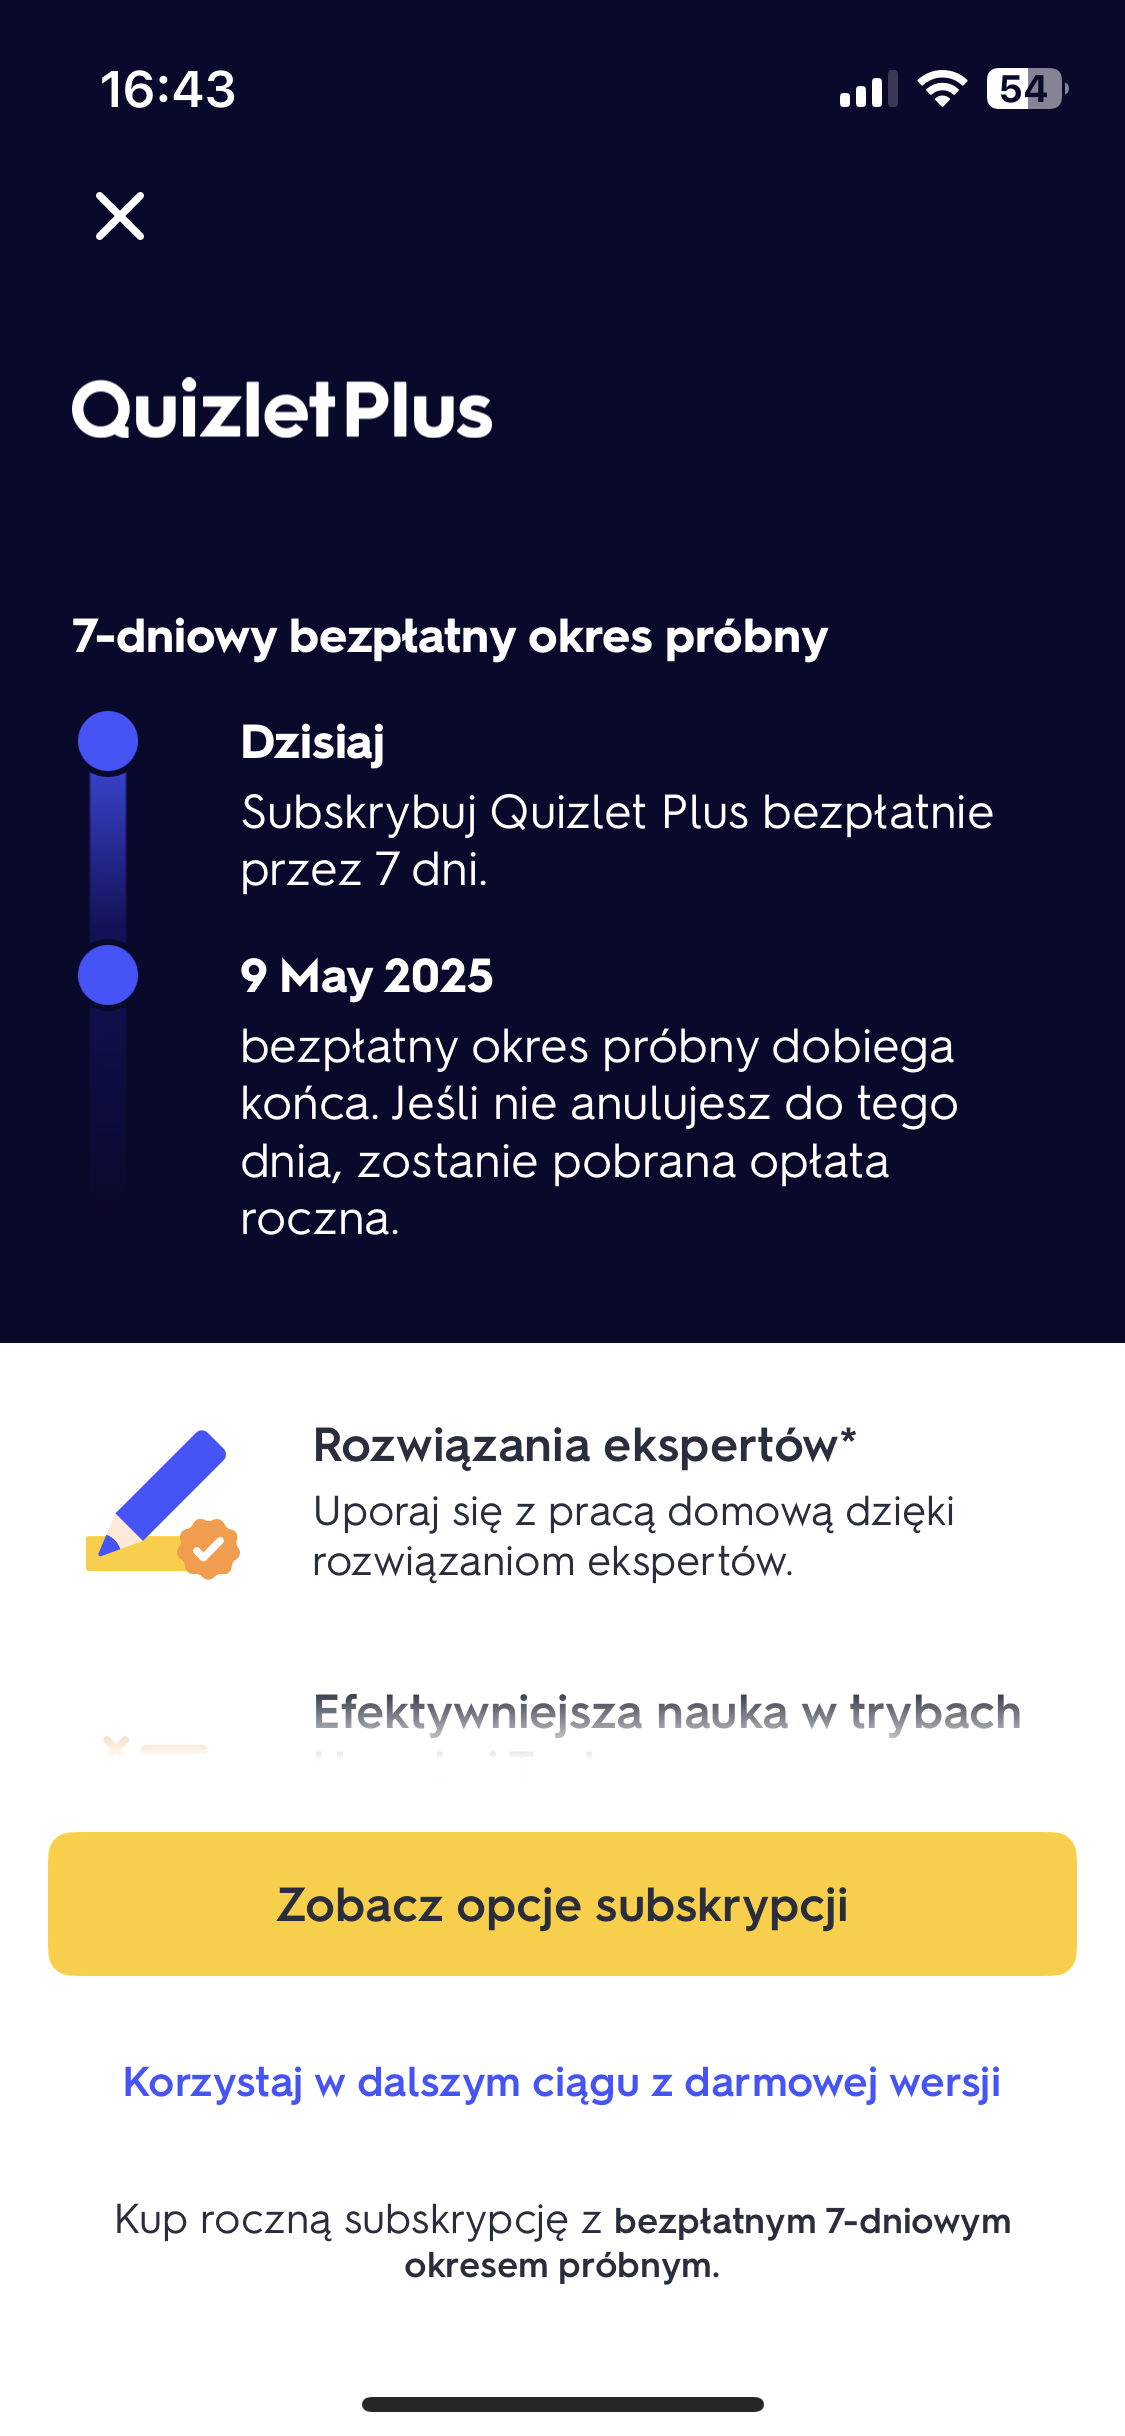
\includegraphics[width=.75\linewidth]{img/quizlet2.PNG}
  \caption{Quizlet: Drugi ekran}
  \label{fig:quizlet2}
\end{minipage}
\end{figure}

Quizlet \cite{quizlet_appstore} to amerykański serwis internetowy do nauki posiadający około 60 milionów użytkowników \cite{quizlet_about}. Umożliwia tworzenie zestawów fiszek oraz udostępnianie ich innym użytkownikom. Istnieje także opcja założenia konta dla nauczycieli, gdzie mogą oni utworzyć klasę i zapraszać do niej swoich uczniów. Ponadto wersja premium aplikacji dodaje dodatkowe funkcjonalności między innymi usuwanie reklam, dodawanie zdjęć do stworzonych fiszek oraz umożliwia zaawansowane formatowanie tekstu. Quizlet dostępny jest w paru formatach: w postaci strony internetowej, a także jako aplikacja na platformy Android oraz iOS. Na potrzeby pracy omawiana zostanie wersja aplikacji na system iOS. 

Do korzystania z aplikacji konieczne jest utworzenie lub zalogowanie się do istniejącego konta. Pierwszą rzeczą widoczną po zalogowaniu jest pełnoekranowy komunikat proponujący zakup subskrypcji o nazwie QuizletPlus. Po wyjściu z widoku subskrypcji w aplikacji pojawia się kolejne okno zalecające włączenie powiadomień. Aplikacja wyświetla dużą ilość elementów zanim pozwoli użytkownikowi na dostęp do swojej głównej funkcjonalności, co może zniechęcić część potencjalnych zainteresowanych do dalszego korzystania z tego serwisu. 

\begin{figure}[H]
\centering
\begin{minipage}{0.5\textwidth}
  \centering
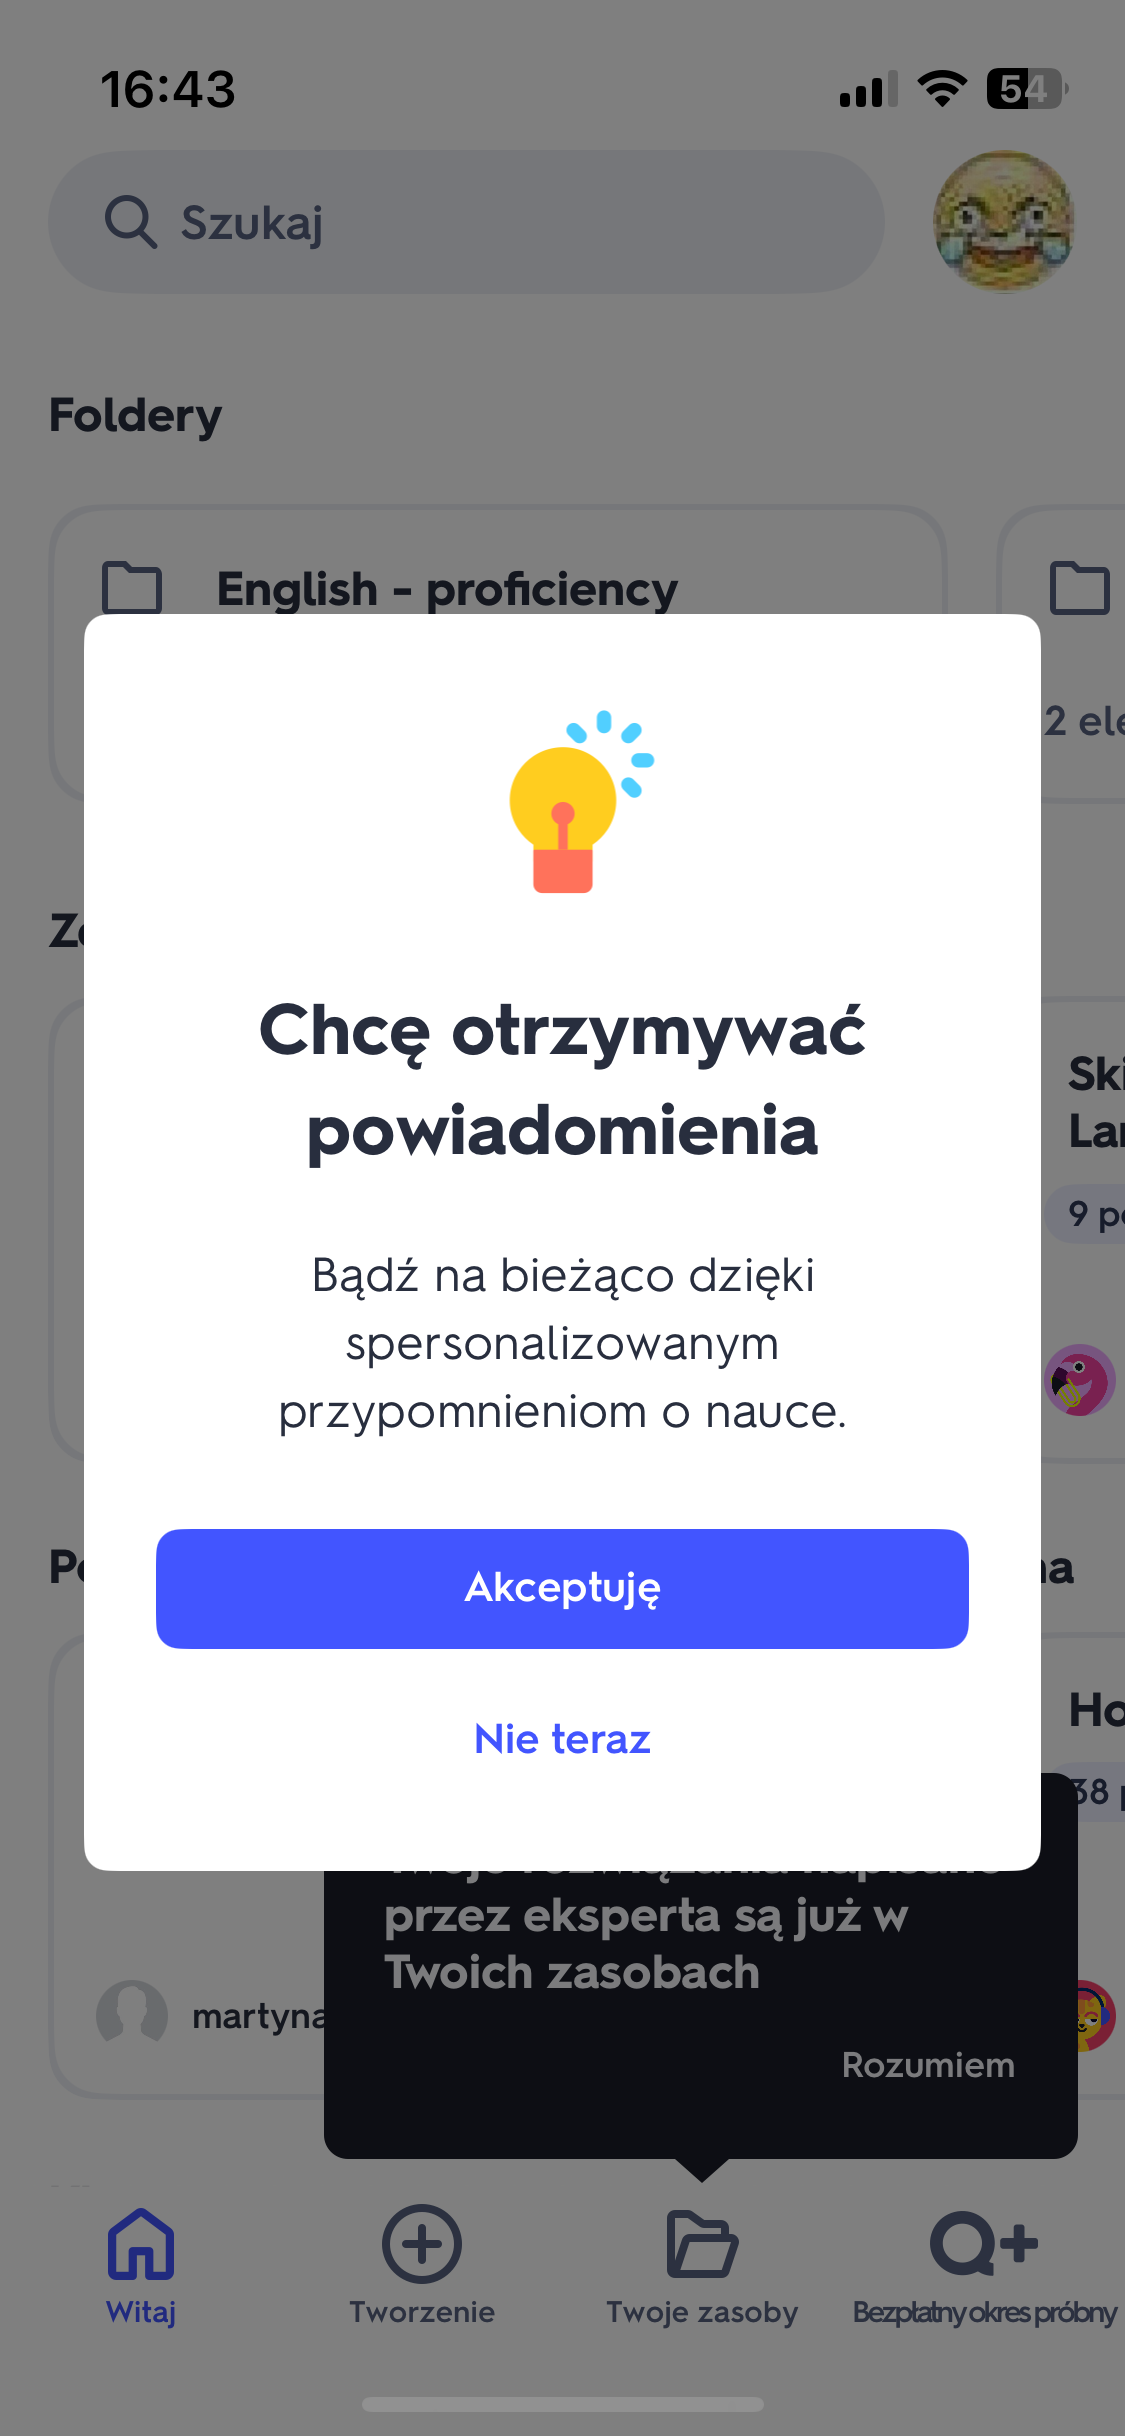
\includegraphics[width=.75\linewidth]{img/quizlet3.PNG}
  \caption{Quizlet: Komunikat wyświetlany po zalogowaniu się}
  \label{fig:quizlet3}
\end{minipage}%
\begin{minipage}{0.5\textwidth}
  \centering
  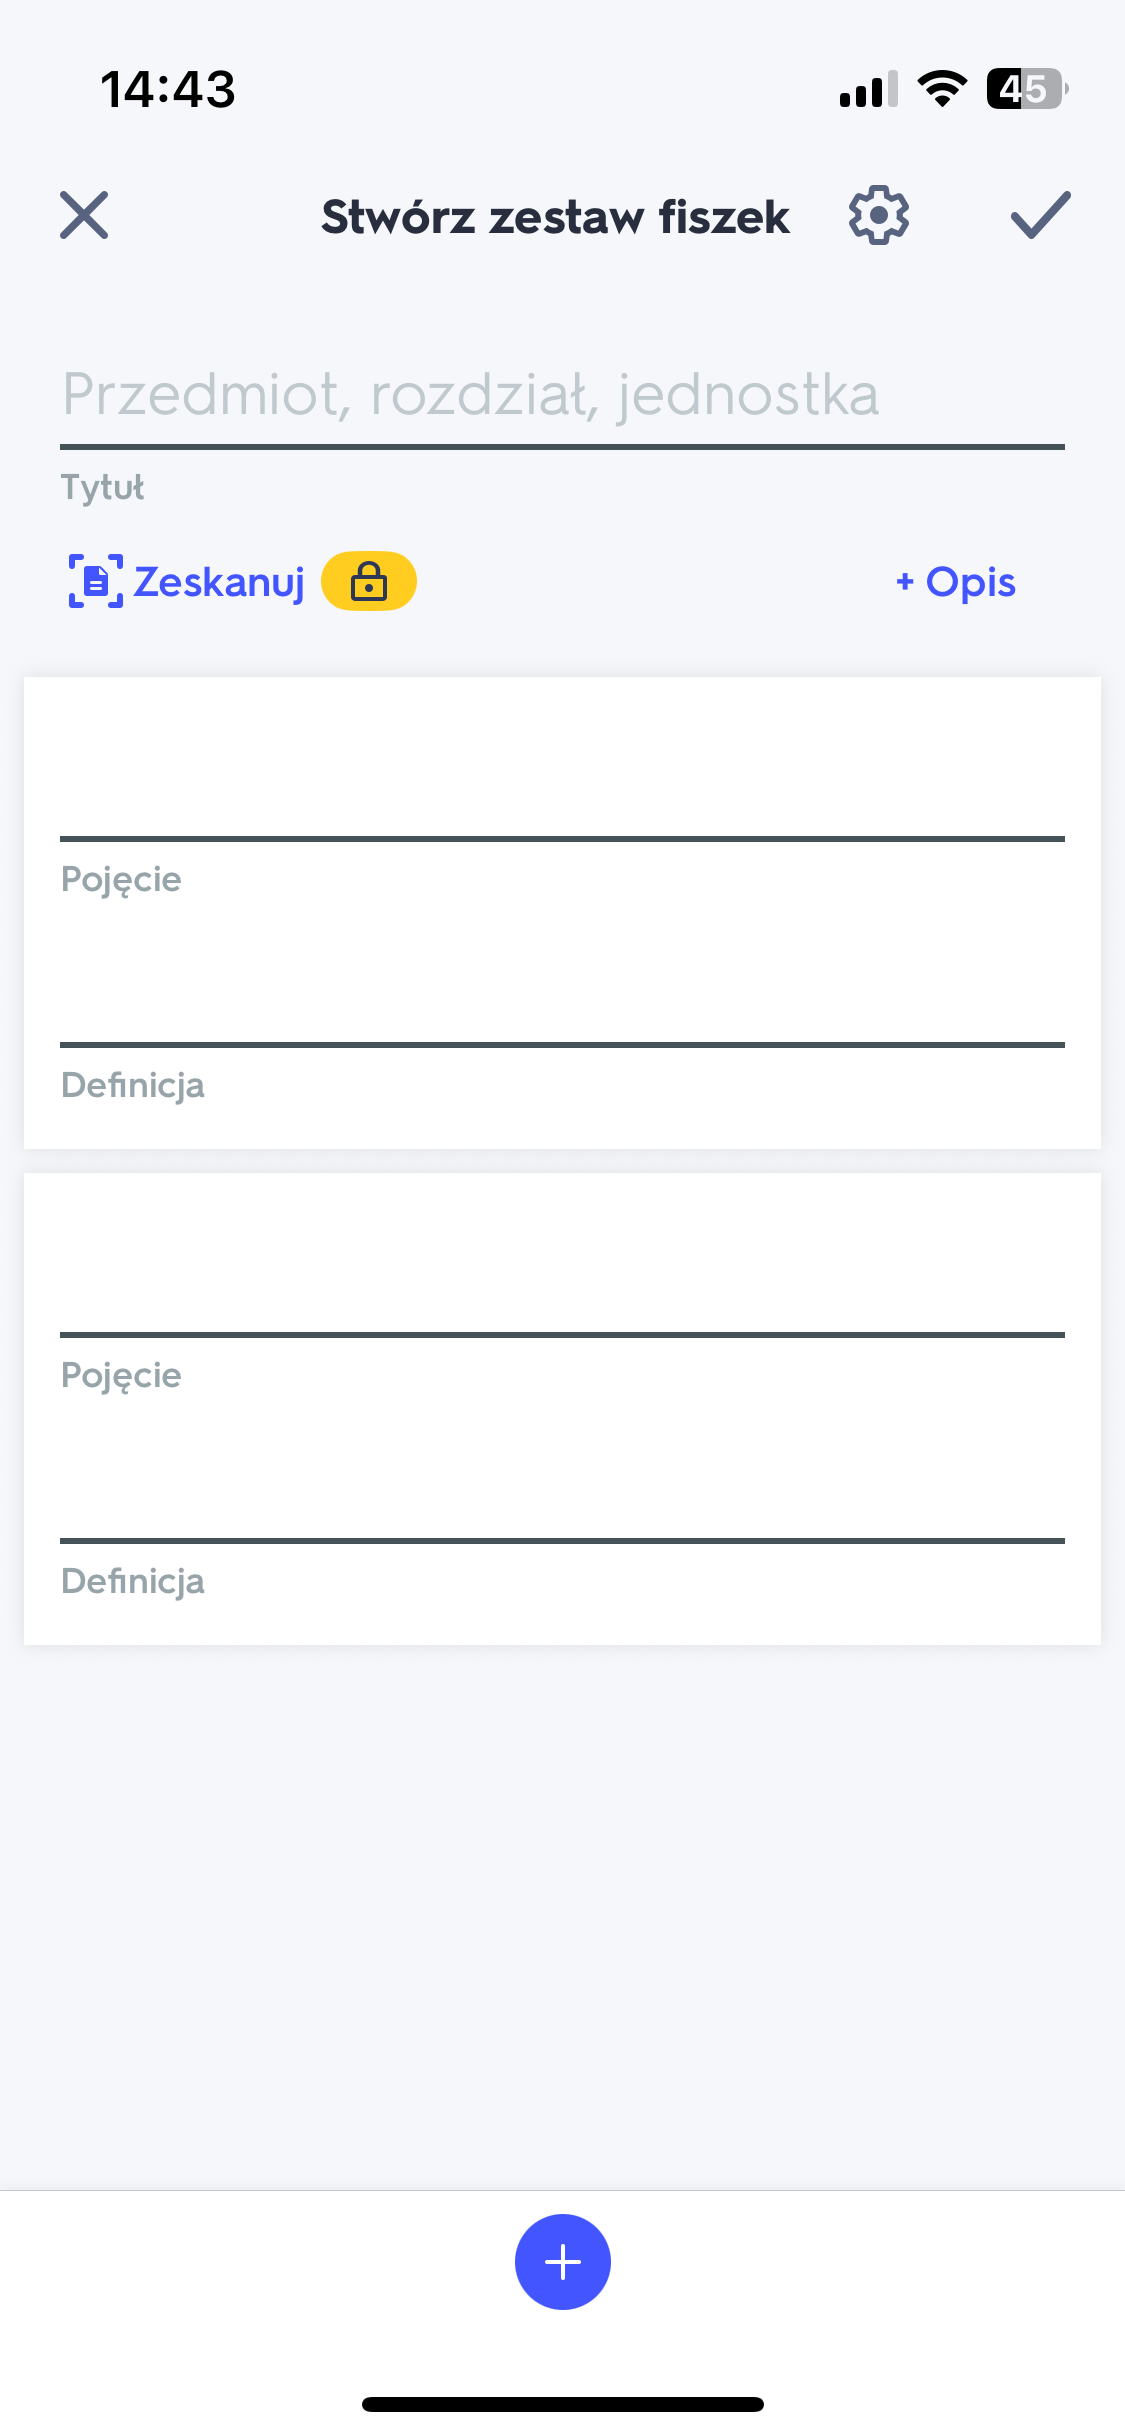
\includegraphics[width=.75\linewidth]{img/quizlet4.PNG}
  \caption{Quizlet: Ekran tworzenia zestawu fiszek}
  \label{fig:quizlet4}
\end{minipage}
\end{figure}

Struktura aplikacji jest podzielona na cztery sekcje używając guzików nawigacyjnych w dolnej części ekranu. Pierwsza z nich to ,,Witaj'', gdzie znajduje się podsumowanie ostatnio używanych i proponowanych zestawów fiszek. Następnie znaleźć można sekcję ,,Tworzenie'', gdzie użytkownik ma możliwość utworzyć zestaw fiszek, folder, albo klasę. Sekcja ,,Twoje zasoby'' daje dostęp do wszystkich utworzonych do tej pory zestawów fiszek. Ostatnia z nich to “Bezpłatny okres próbny” dająca możliwość zakupu wersji premium aplikacji za pomocą subskrypcji QuizletPlus. Propozycja zakupu subskrypcji wyświetla się nie tylko tutaj, lecz także w innych miejscach aplikacji. Przy przyciskach oferujących funkcjonalności dostępne wyłącznie w wersji premium wyświetla się dymek zachęcający użytkownika do zakupienia QuizletPlus. 

\section{AnkiMobile Flashcards}

\begin{figure}[H]
\centering
\begin{minipage}{0.5\textwidth}
  \centering
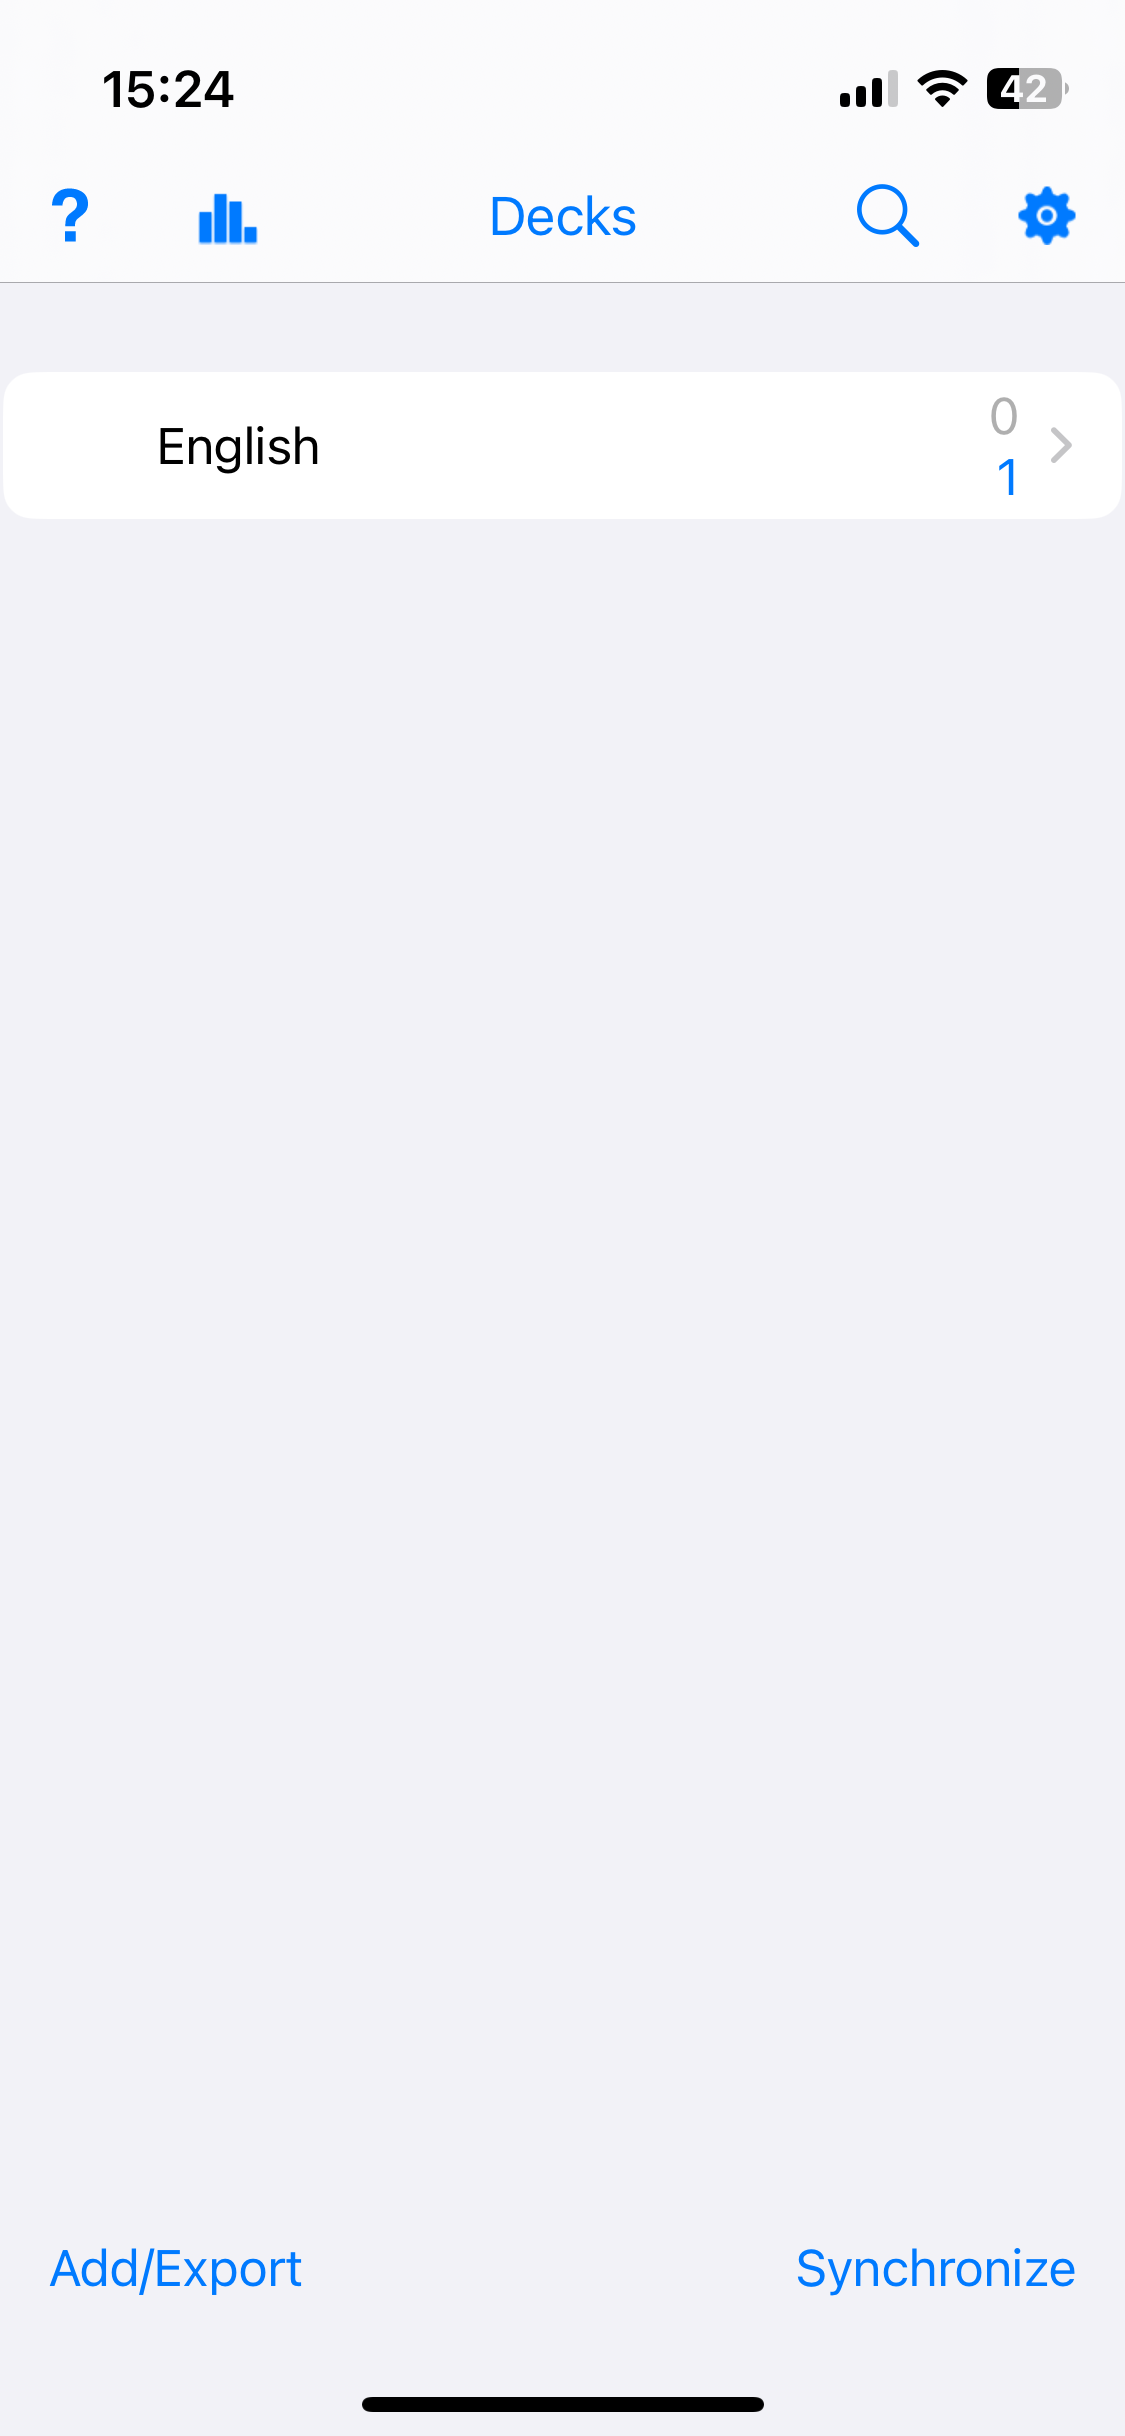
\includegraphics[width=.75\linewidth]{img/anki1.PNG}
  \caption{Anki: Ekran główny}
  \label{fig:anki1}
\end{minipage}%
\begin{minipage}{0.5\textwidth}
  \centering
  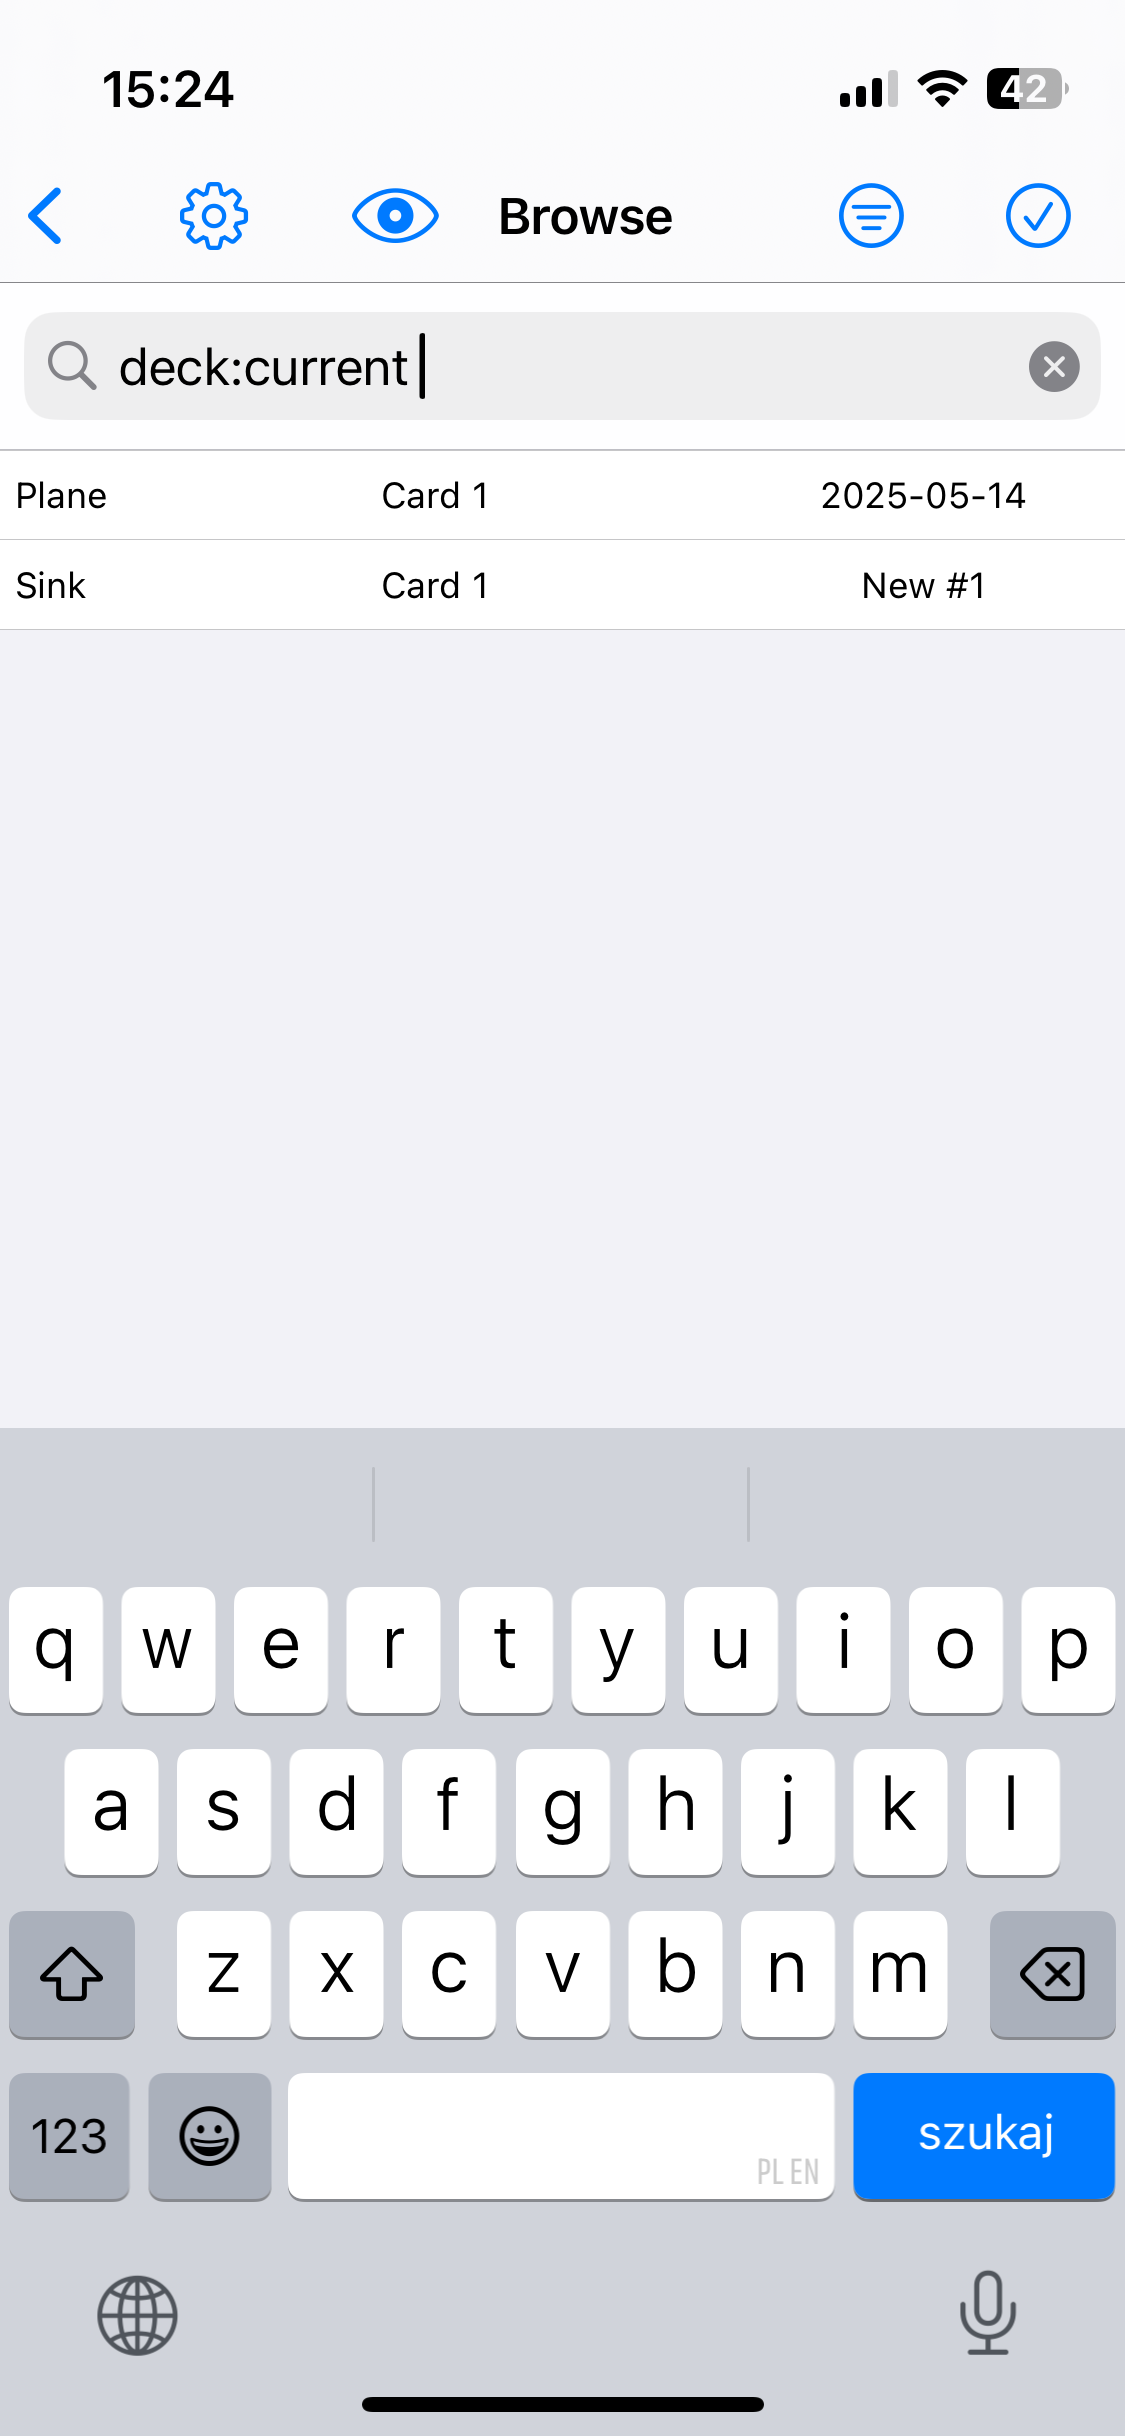
\includegraphics[width=.75\linewidth]{img/anki2.PNG}
  \caption{Anki: Lista fiszek wewnątrz zestawu fiszek}
  \label{fig:anki2}
\end{minipage}
\end{figure}

Anki \cite{anki_appstore} jest open-source programem do tworzenia fiszek współgrającym z darmowym portalem AnkiWeb, dzięki któremu można zapisywać je w chmurze. Program reklamuje się wykorzystaniem specjalnego algorytmu dobierania fiszek w trakcie nauki, aby optymalizować ich zapamiętywanie. Bazuje on na algorytmie SuperMemo 2 \cite{anki_algo}. Darmowa wersja aplikacji dostępna jest na platformę Android, natomiast wersja na system iOS kosztuje 129,99 zł. Cena ta jest stosunkowo wysoka w porównaniu z innymi aplikacjami w tej kategorii.

Po włączeniu aplikacja nie wymaga konta do tworzenia fiszek, użytkownik od razu dostaje dostęp do domyślnego ekranu aplikacji, gdzie widoczne są zestawy fiszek. Po wejściu w dany zestaw wyświetlany zostaje ekran nauczania umożliwiający naukę lub dodawanie nowych fiszek. Każdą z fiszek można uzupełnić mediami o różnych formatach. Oprócz sformatowanego tekstu lub zdjęcia, treść może być przedstawiona w postaci nagrania audio, rysunku, działania matematycznego, bloku kodu lub nawet załącznika. Wersje aplikacji na systemy macOS, Windows oraz Linux dają możliwość rozszerzenia obszernej już funkcjonalności Anki za pomocą wtyczek, lecz niestety nie jest to możliwe w aplikacji mobilnej AnkiMobile. 
    
Aplikacja charakteryzuje się dość surowym wyglądem, większość interfejsu użytkownika składa się z domyślnych elementów dostępnych w systemie iOS. W AnkiMobile ilość dostępnych funkcjonalności zdaje się grać większą rolę, niż intuicyjność obsługi. Przykładem tego może być zestaw fiszek --- po wejściu do uprzednio dodanego zestawu użytkownik od razu umieszczany jest w trybie nauki, nawet jeśli zestaw nie posiada jeszcze żadnych elementów. Pusty zestaw gratuluje użytkownikowi pomyślnego skończenia nauki, co może powodować zdezorientowanie osób korzystających z aplikacji po raz pierwszy. Dodatkowo aplikacja nie posiada żadnego przewodnika lub wskazówek informujących użytkownika o sposobie dodawania nowych fiszek.

\begin{figure}[H]
\centering
\begin{minipage}{0.5\textwidth}
  \centering
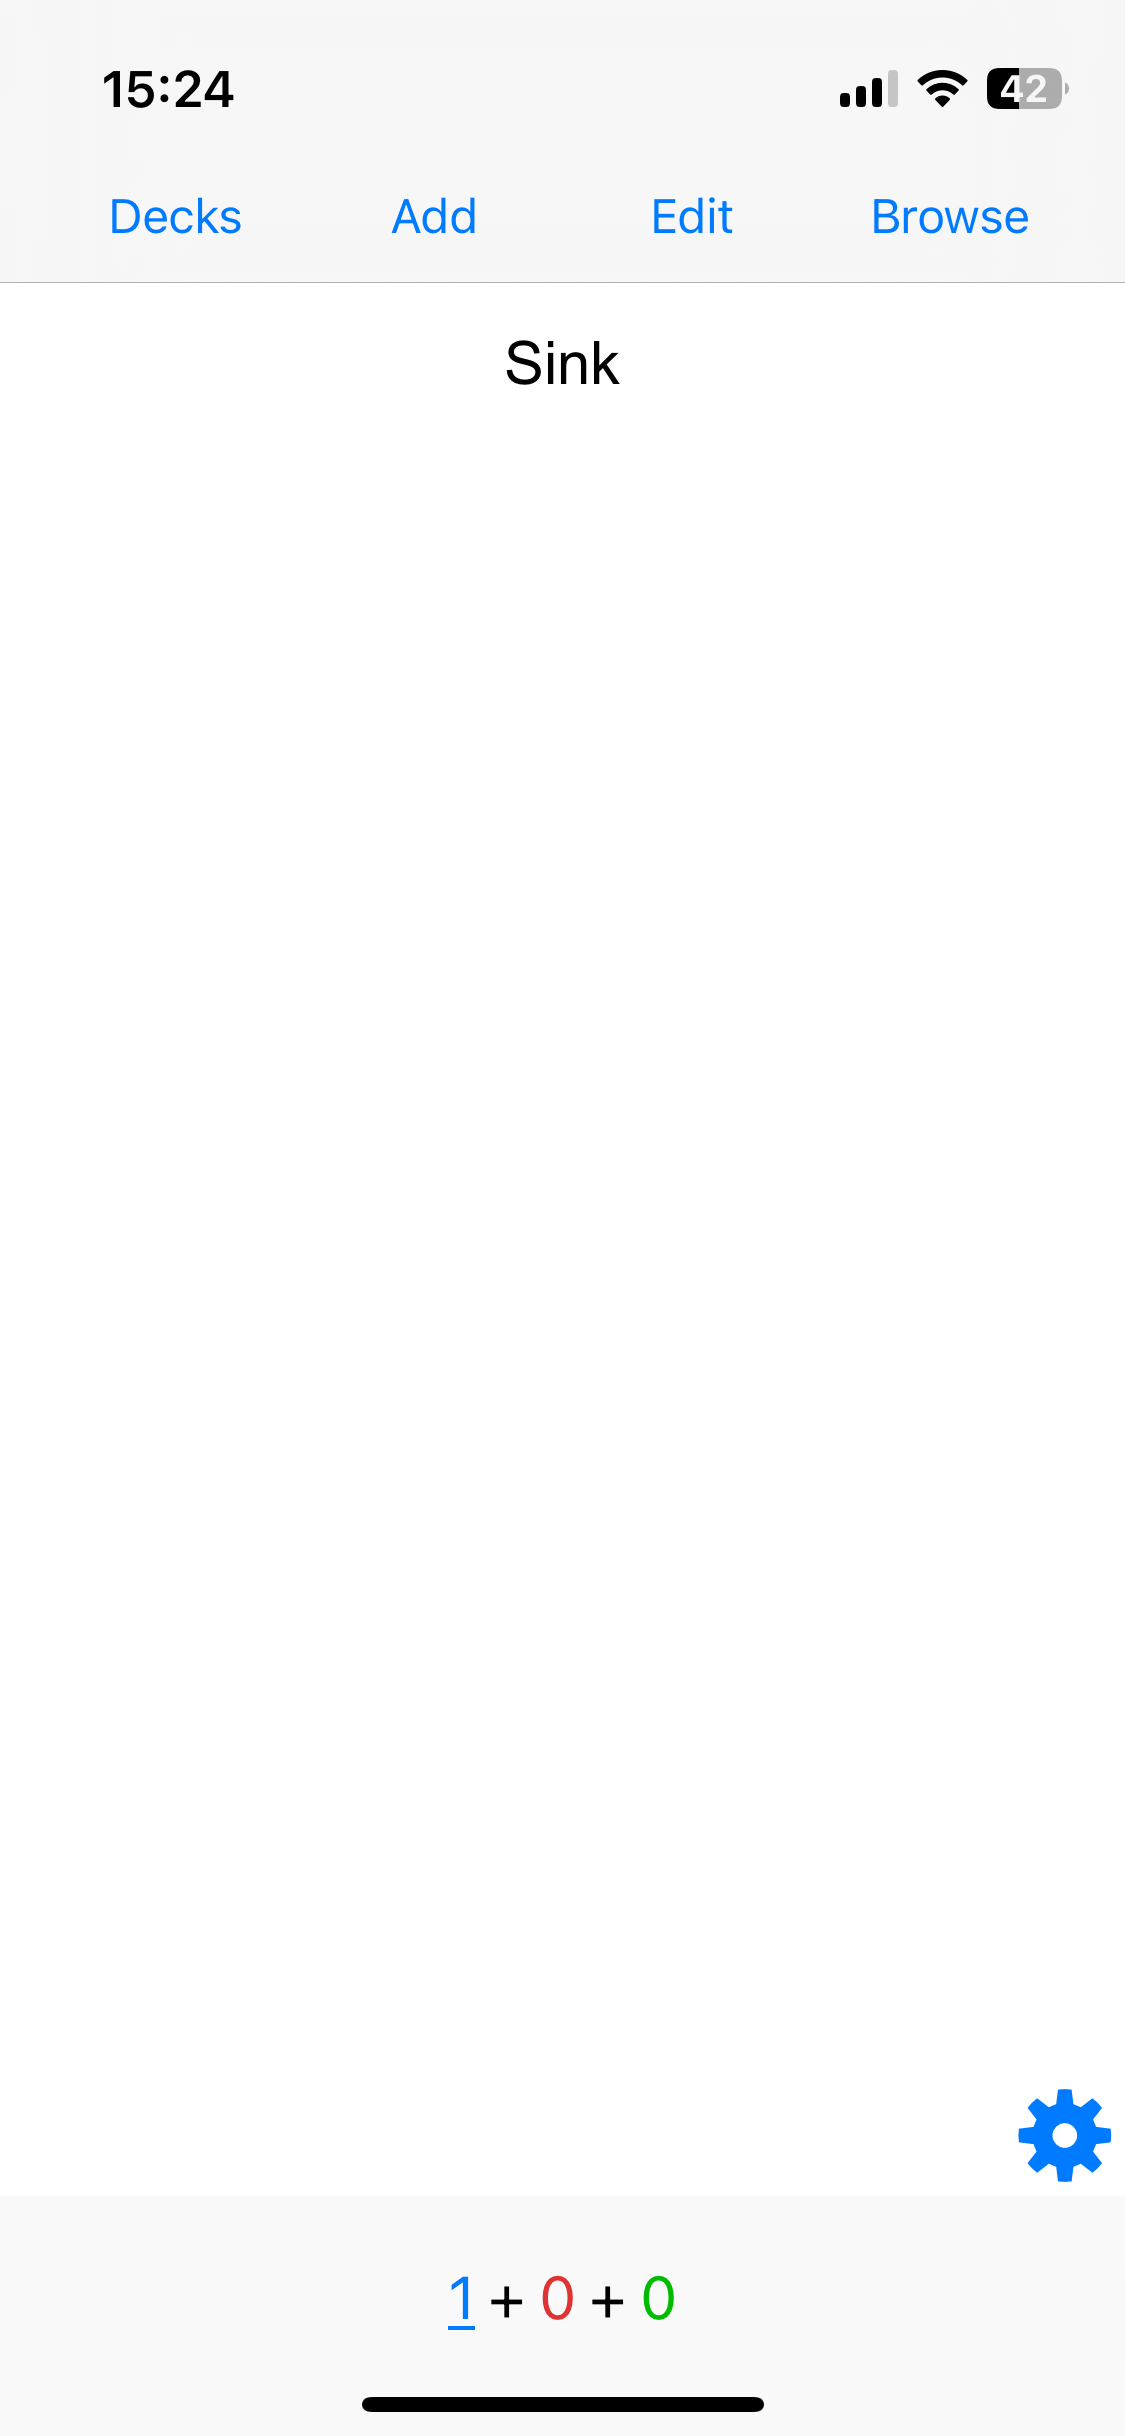
\includegraphics[width=.75\linewidth]{img/anki3.PNG}
  \caption{Anki: Widok fiszki}
  \label{fig:anki3}
\end{minipage}%
\begin{minipage}{0.5\textwidth}
  \centering
  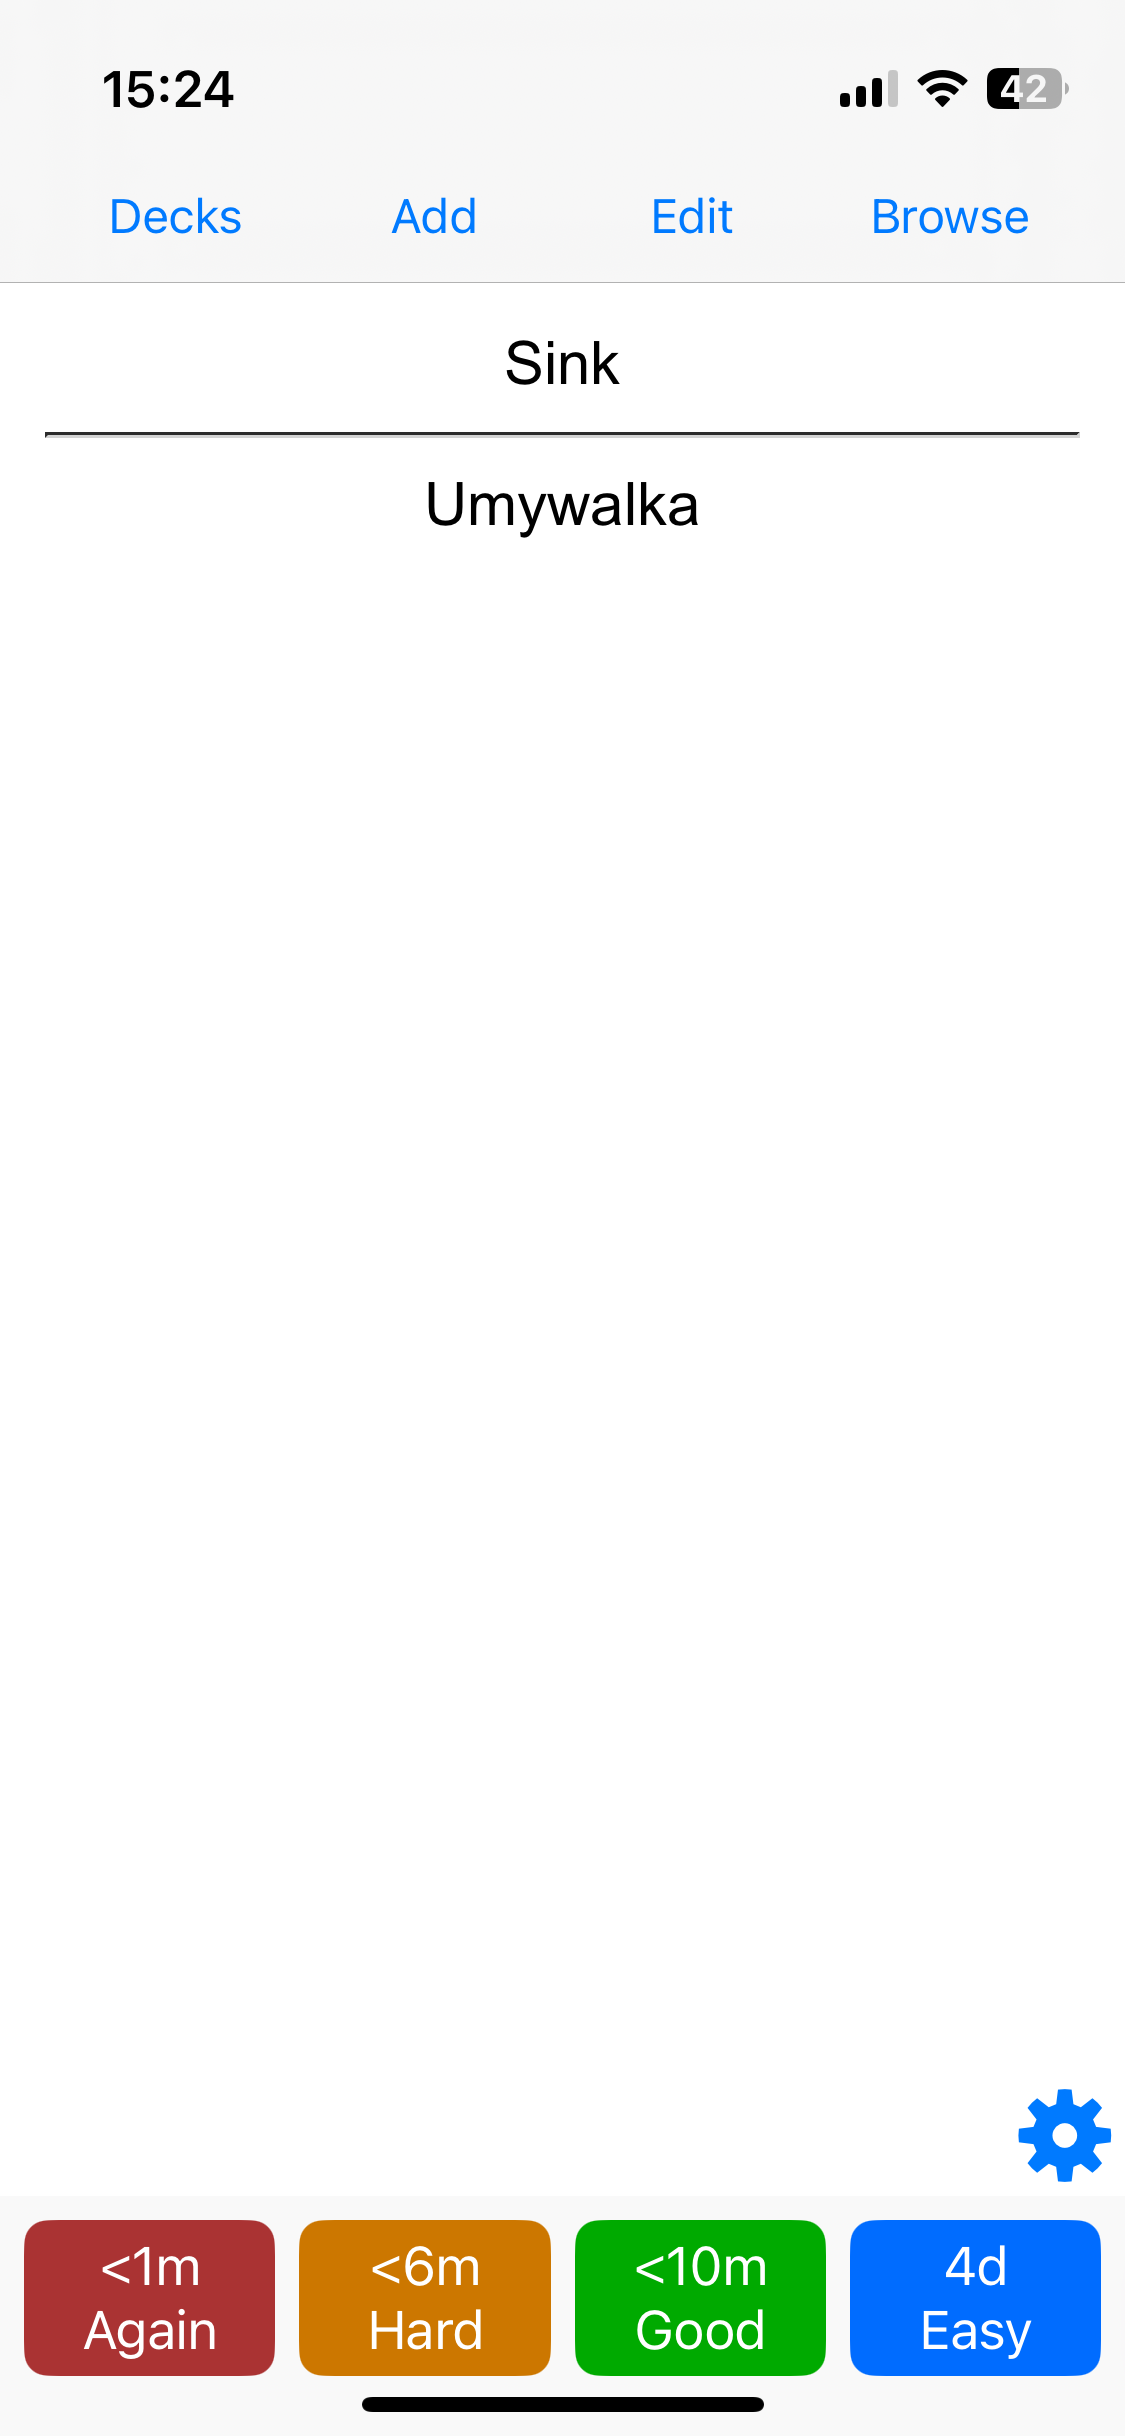
\includegraphics[width=.75\linewidth]{img/anki4.PNG}
  \caption{Anki: Widok fiszki po kliknięciu}
  \label{fig:anki4}
\end{minipage}
\end{figure}

\section{FlashCards}

\begin{figure}[H]
\centering
\begin{minipage}{0.5\textwidth}
  \centering
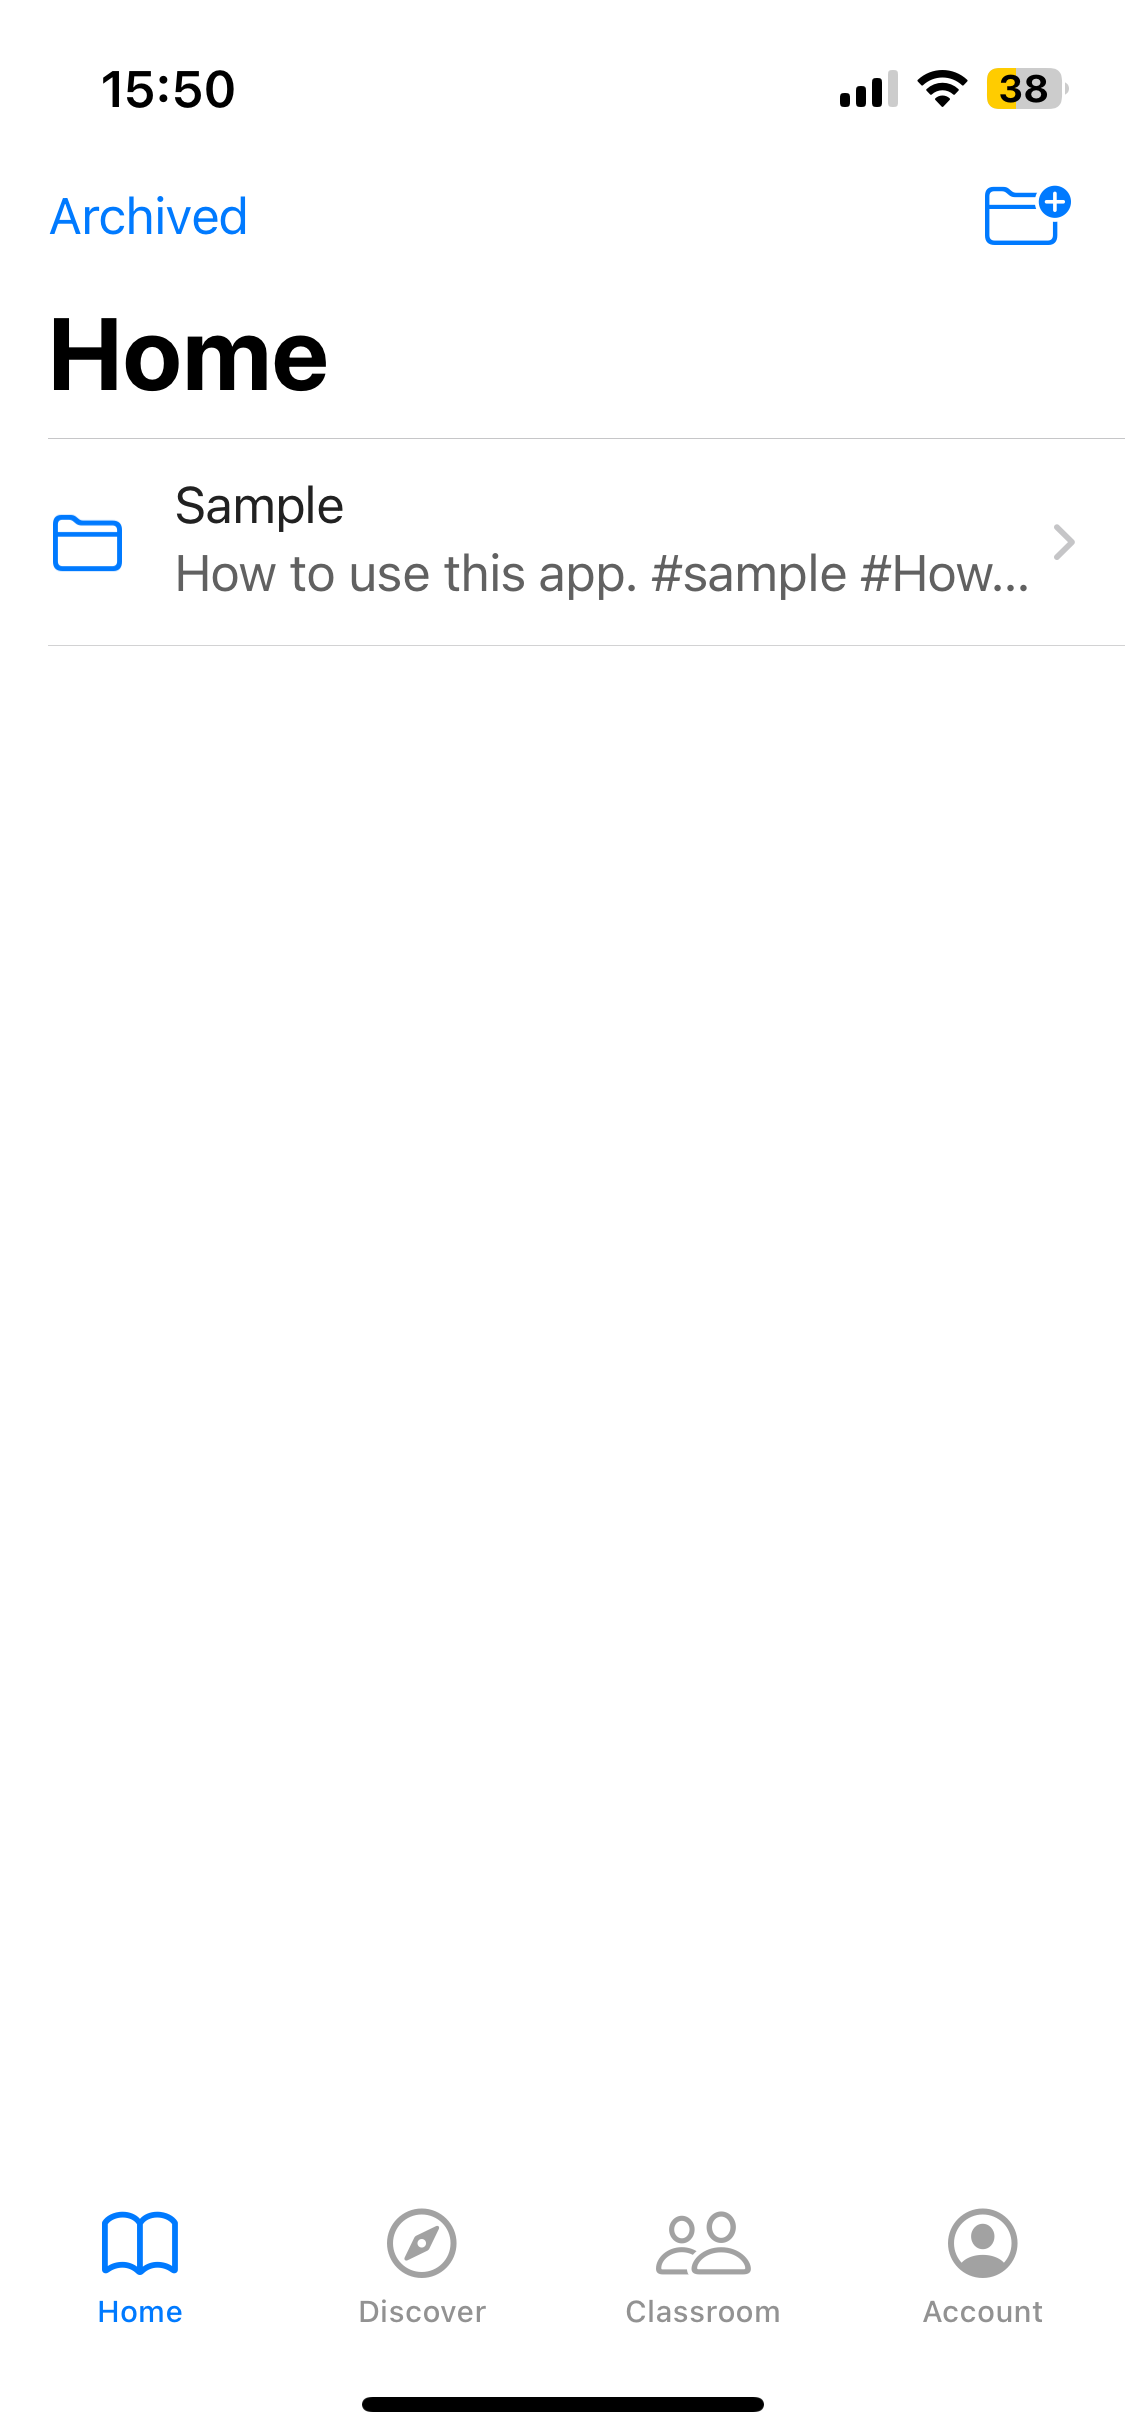
\includegraphics[width=.75\linewidth]{img/flashcards1.PNG}
  \caption{FlashCards: Ekran główny}
  \label{fig:flashcards1}
\end{minipage}%
\begin{minipage}{0.5\textwidth}
  \centering
  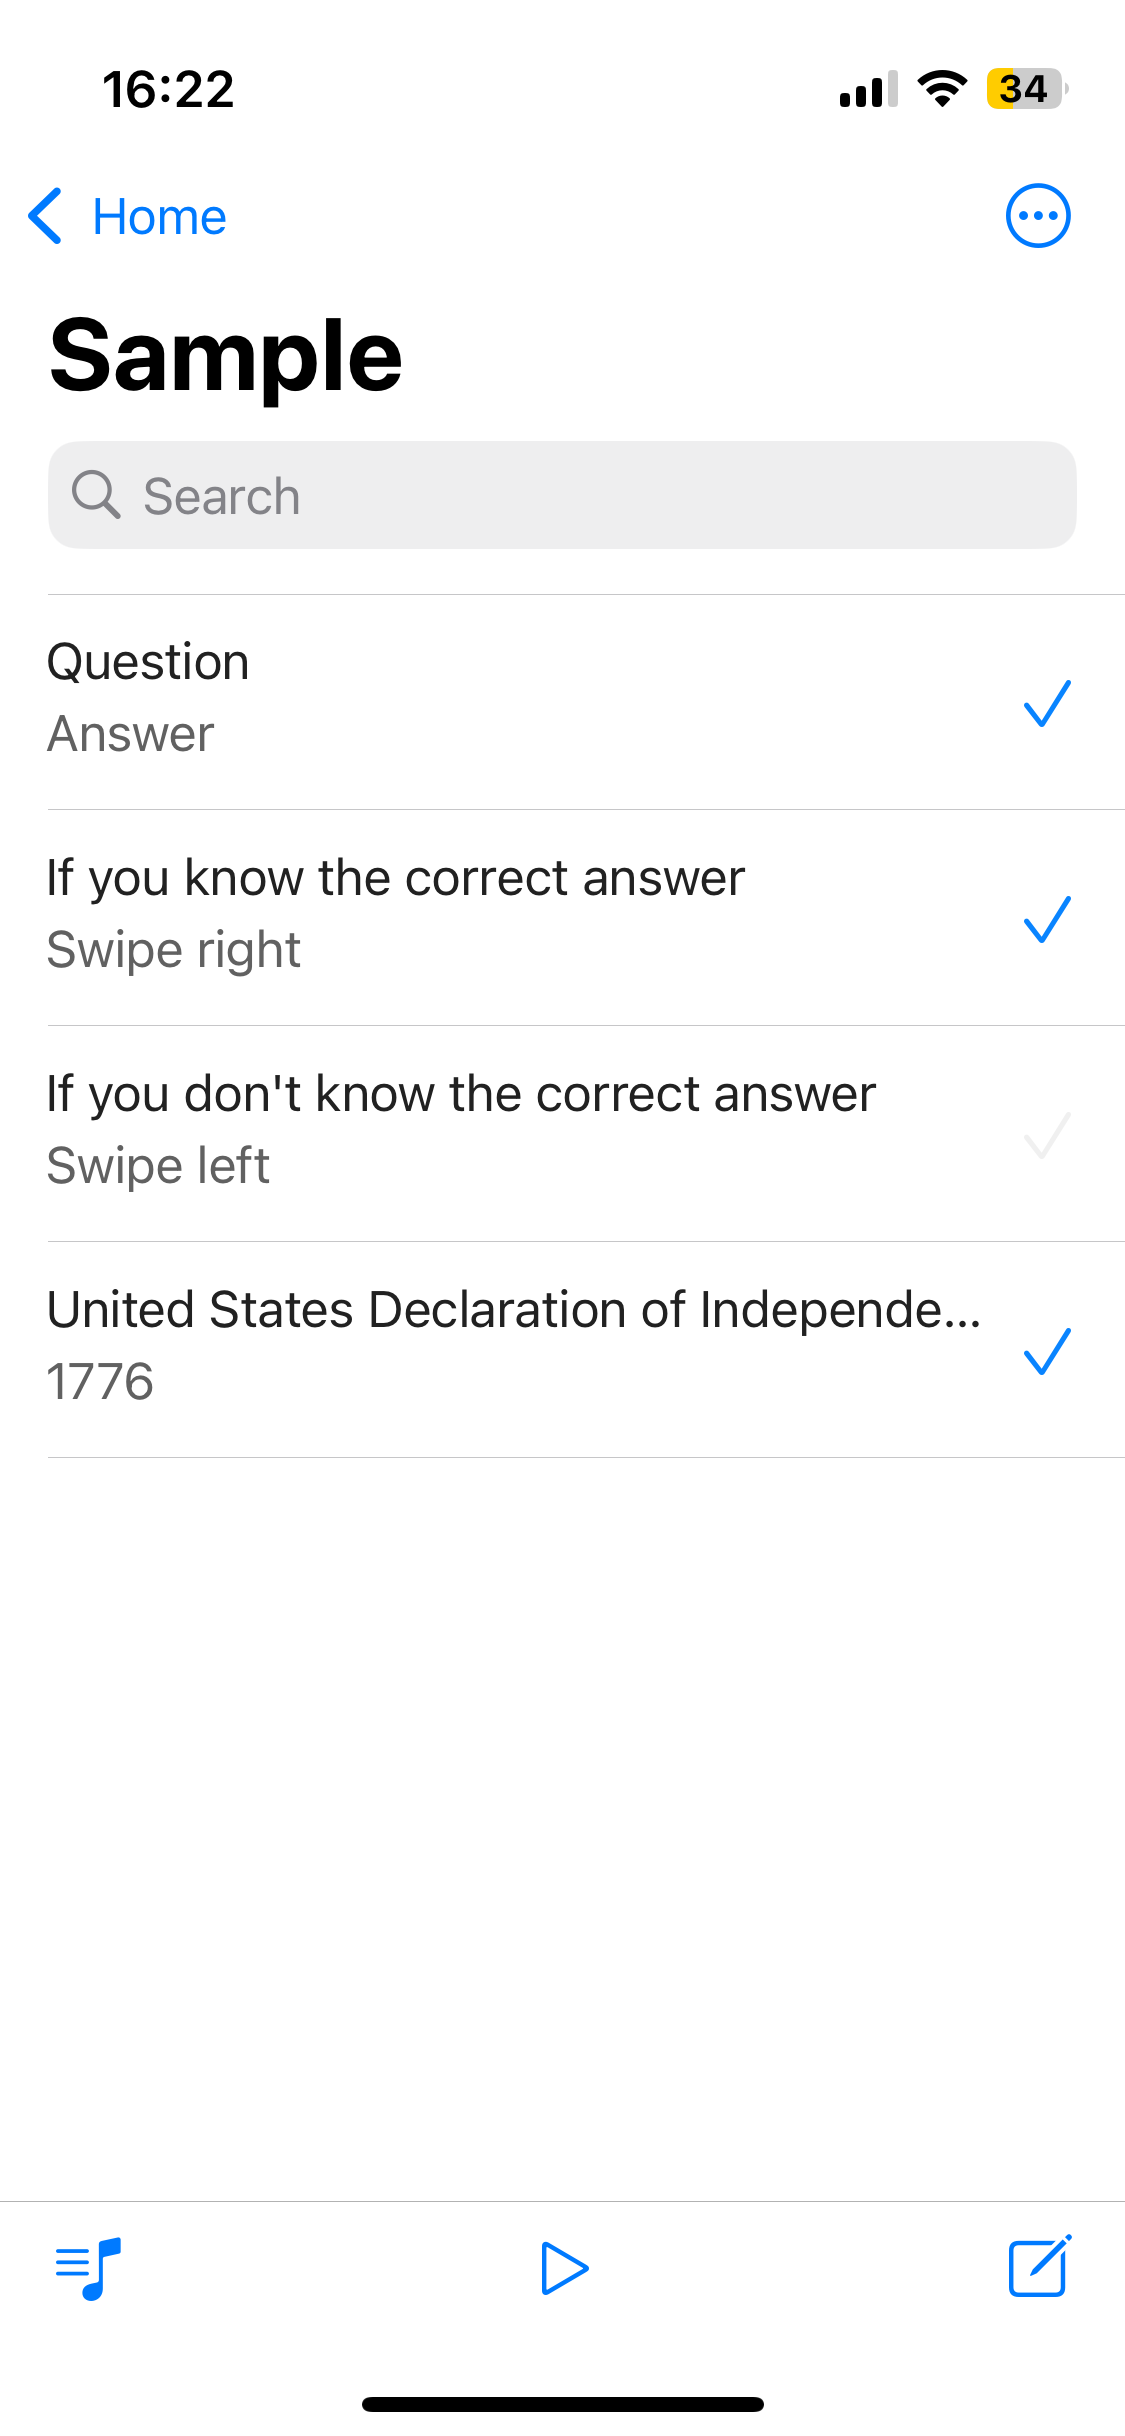
\includegraphics[width=.75\linewidth]{img/flashcards2.PNG}
  \caption{FlashCards: Widok przykładowego zestawu fiszek}
  \label{fig:flashcards2}
\end{minipage}
\end{figure}

FlashCards \cite{flashcards_appstore} to aplikacja, której autorem jest osoba posiadająca konto deweloperskie w sklepie App Store o nazwie Toshiki Motomura. Jako kolejna charakteryzuje się prostotą wyglądu stawiającym na użycie podstawowych elementów udostępnianych przez system iOS. Oprócz podstawowych funkcjonalności aplikacja posiada także możliwość dzielenia się swoimi zestawami fiszek z innymi użytkownikami.

Pierwszym ekranem widocznym po otwarciu aplikacji jest sekcja ,,Home'' wyświetlająca wszystkie zestawy fiszek utworzone dotychczas przez użytkownika. Na start udostępniany jest domyślny zestaw z przykładowymi pojęciami. Następnie za pomocą dolnego paska nawigacji przejść można do sekcji ,,Discover'', gdzie jak już wcześniej wspomniano użytkownik znaleźć może zestawy fiszek utworzone przez inne osoby korzystające z aplikacji. Kolejną sekcją jest ,,Classroom'' --- udostępnia możliwość tworzenia prywatnych grup wewnątrz, których użytkownicy mają szansę dzielić się swoimi fiszkami. Ostatnią sekcją na pasku nawigacji jest ,,Account'', gdzie można znaleźć ustawienia aplikacji.

\begin{figure}[H]
\centering
\begin{minipage}{0.5\textwidth}
  \centering
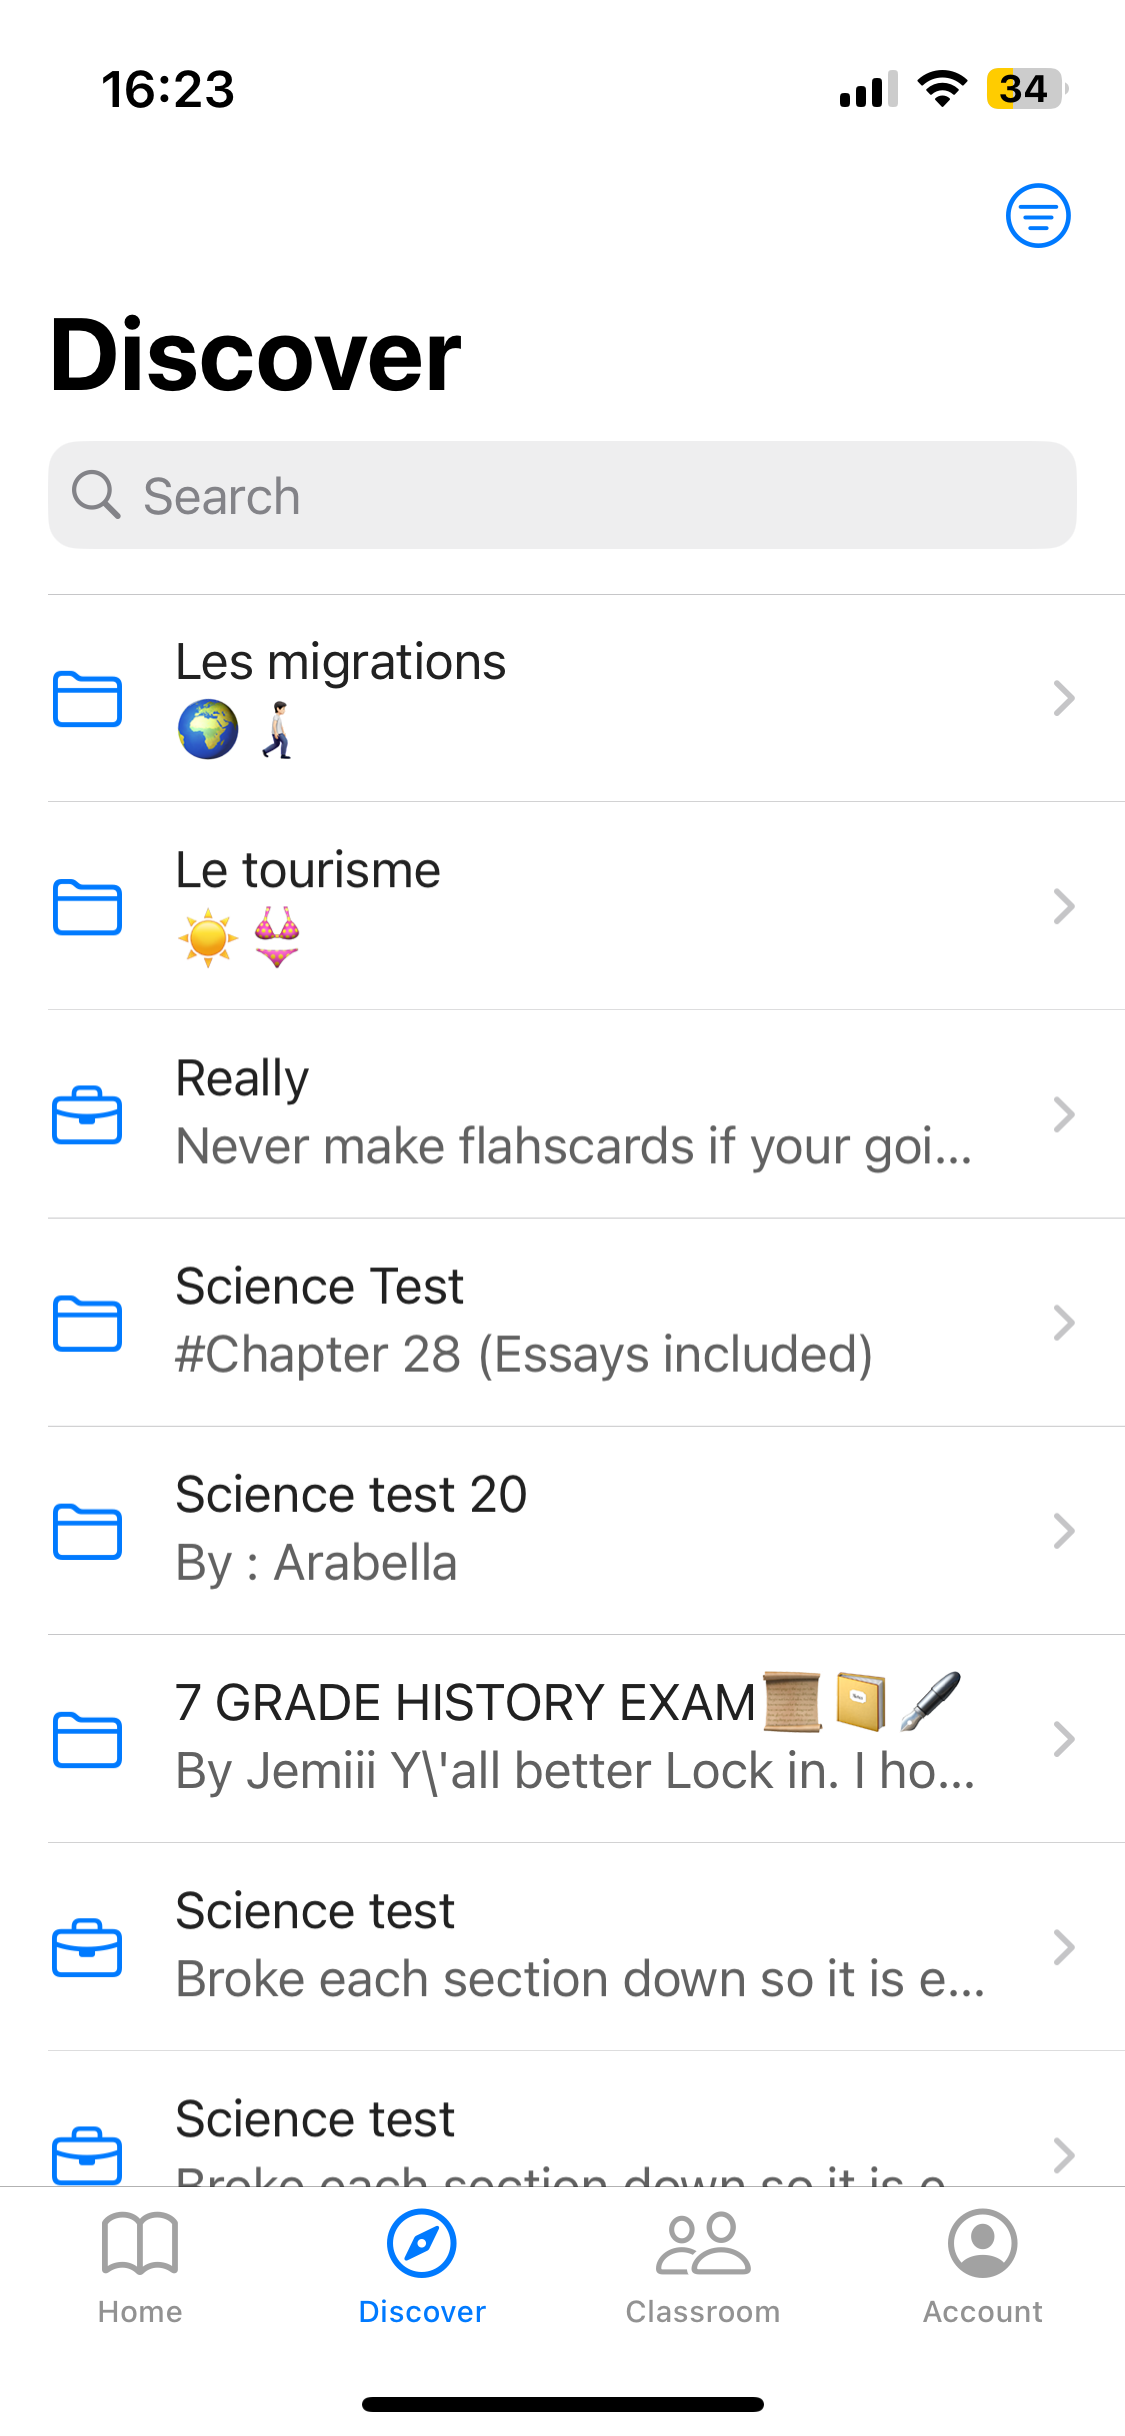
\includegraphics[width=.75\linewidth]{img/flashcards3.PNG}
  \caption{FlashCards: Sekcja z zestawami udostępnianymi przez innych użytkowników}
  \label{fig:flashcards3}
\end{minipage}%
\begin{minipage}{0.5\textwidth}
  \centering
  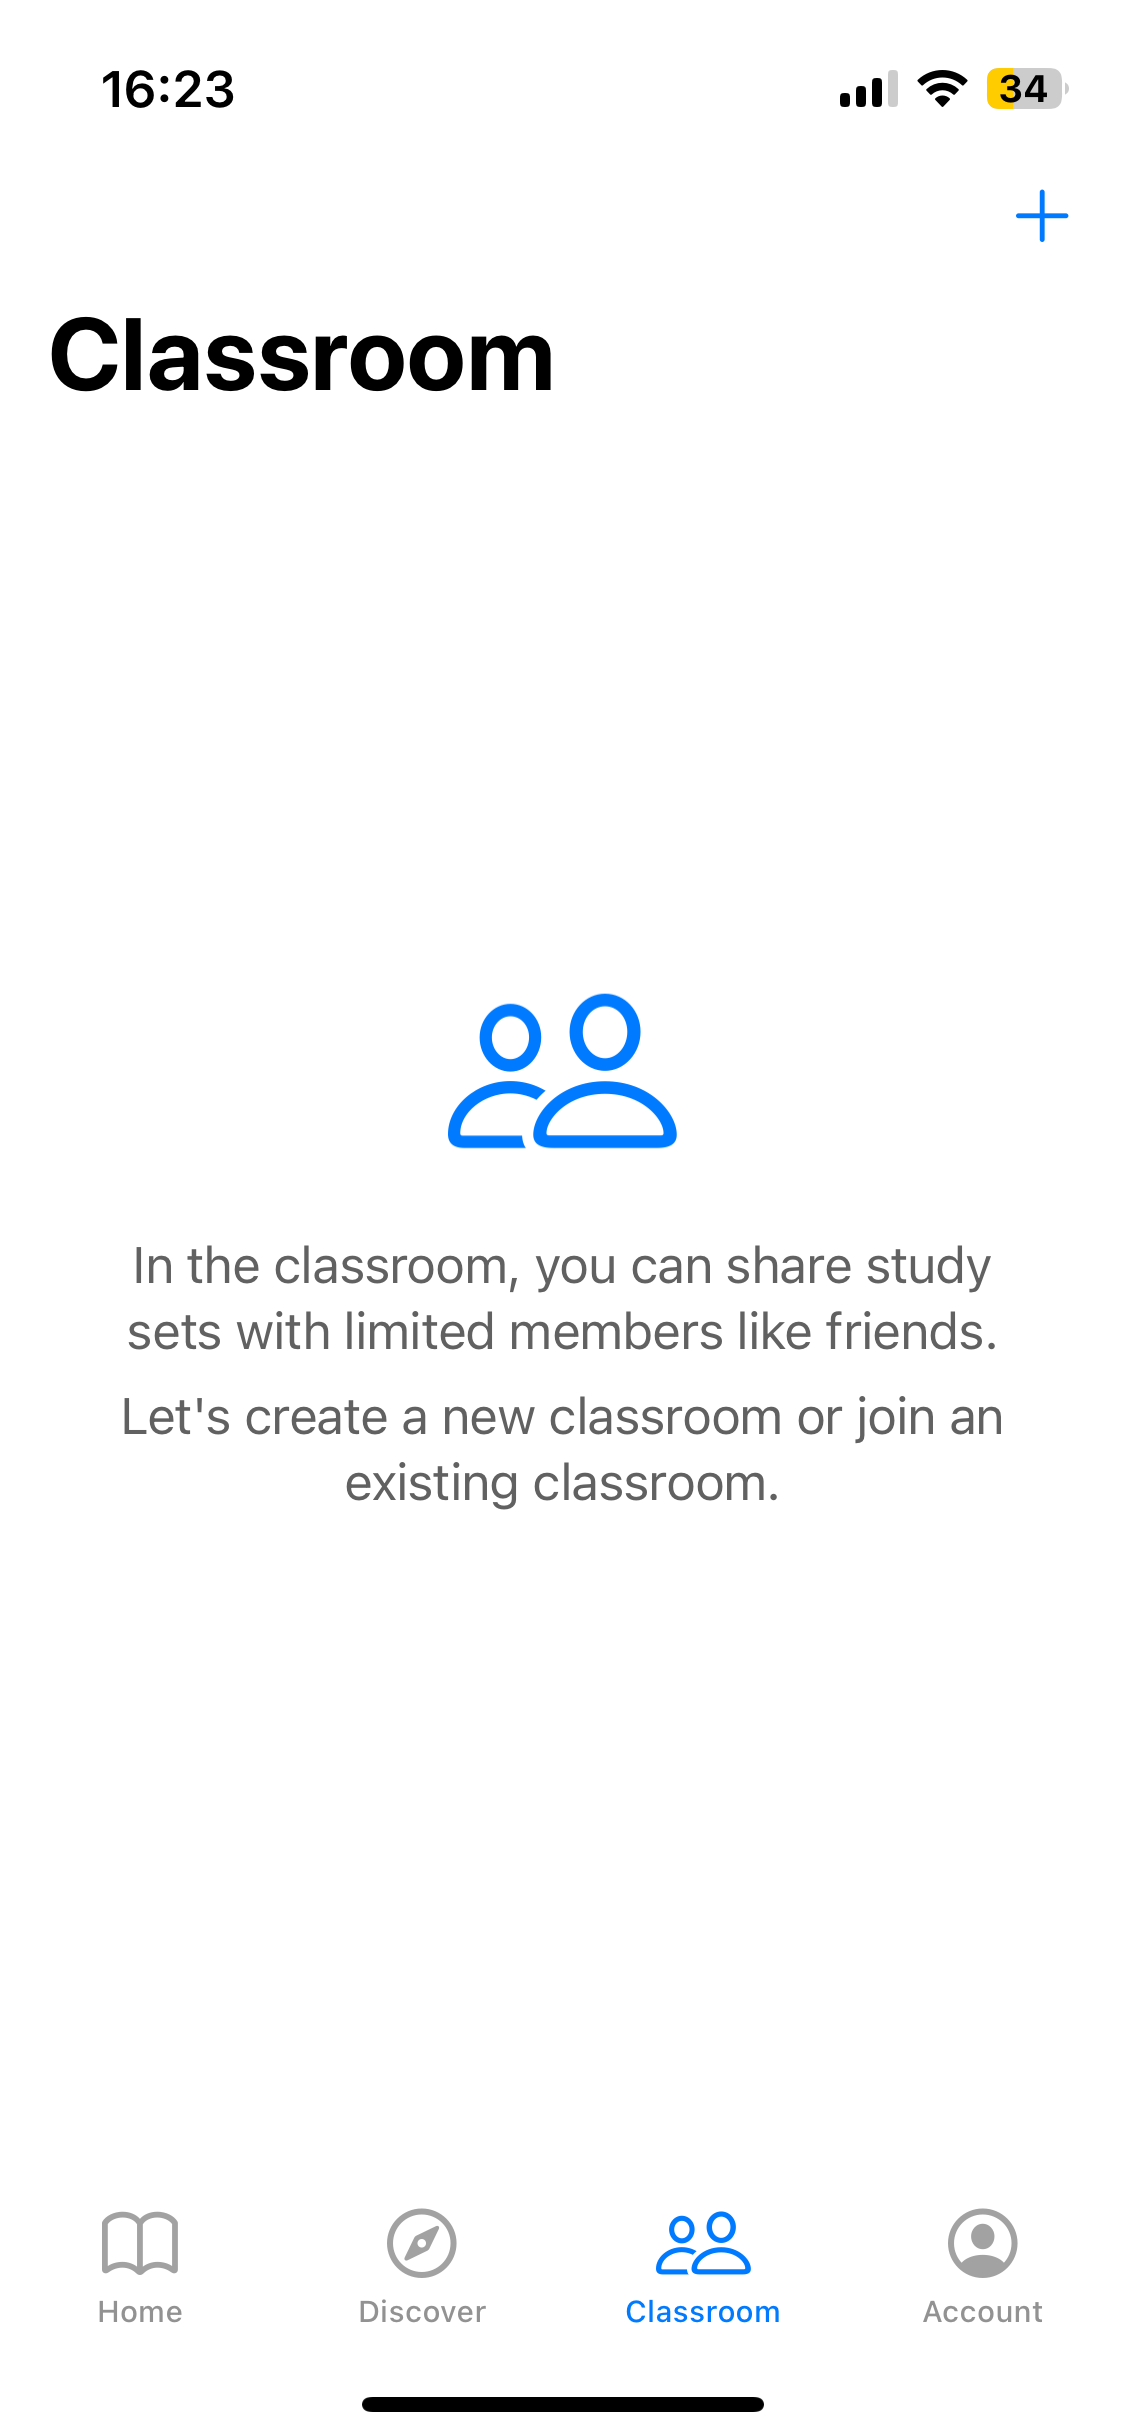
\includegraphics[width=.75\linewidth]{img/flashcards4.PNG}
  \caption{FlashCards: Sekcja pozwalająca na utworzenie klasy}
  \label{fig:flashcards4}
\end{minipage}
\end{figure}

\section{Flashcards maker}


Flashcard maker \cite{flashcards_maker_appstore} to kolejna aplikacja autorstwa niezależnego dewelopera ---- w tym wypadku jest to Yoshinobu Ikeda. Wyróżnia się na tle innych opisanych w tym rozdziale aplikacji przede wszystkim swoim wyglądem --- użycie jaskrawych kolorów oraz układ strony głównej i okienek sprawia, że nie pasuje ona do zwyczajnego stylu aplikacji iOS. Kolejną cechą charakterystyczną jest nastawienie na naukę języków. Podczas tworzenia zestawu fiszek aplikacja pyta o dwa języki, między którymi będzie ten zestaw tłumaczył.

Po otwarciu aplikacji Flashcard maker widoczna jest lista zestawów fiszek z przykładowym zestawem do nauki języka hiszpańskiego. Pod nim znajduje się guzik umożliwiający utworzenie nowego zestawu. Aplikacja posiada kilka trybów nauki: test wielokrotnego wyboru, test pisowni, oraz tryb samodzielnego sprawdzania. Pierwszy z nich polega na wyborze popranej odpowiedzi z 4 potencjalnych wybranych losowo z danego katalogu fiszek, natomiast drugi sprawdza pisownię użytkownika poprzez wpisanie frazy w innym języku litera po literze. Ostatni tryb działa analogicznie do trybu dostępnego w aplikacji będącej tematem pracy --- na ekranie ukazuje się karta z frazą, która odwraca się po kliknięciu pokazując jej tłumaczenie. Jeśli odpowiedź użytkownika była poprawna zaznacza on przycisk  ,,\checkmark''. Dodatkowo frazy pokazane na kartach czytane są automatycznie. 


\begin{figure}[H]
\centering
\begin{minipage}{0.5\textwidth}
  \centering
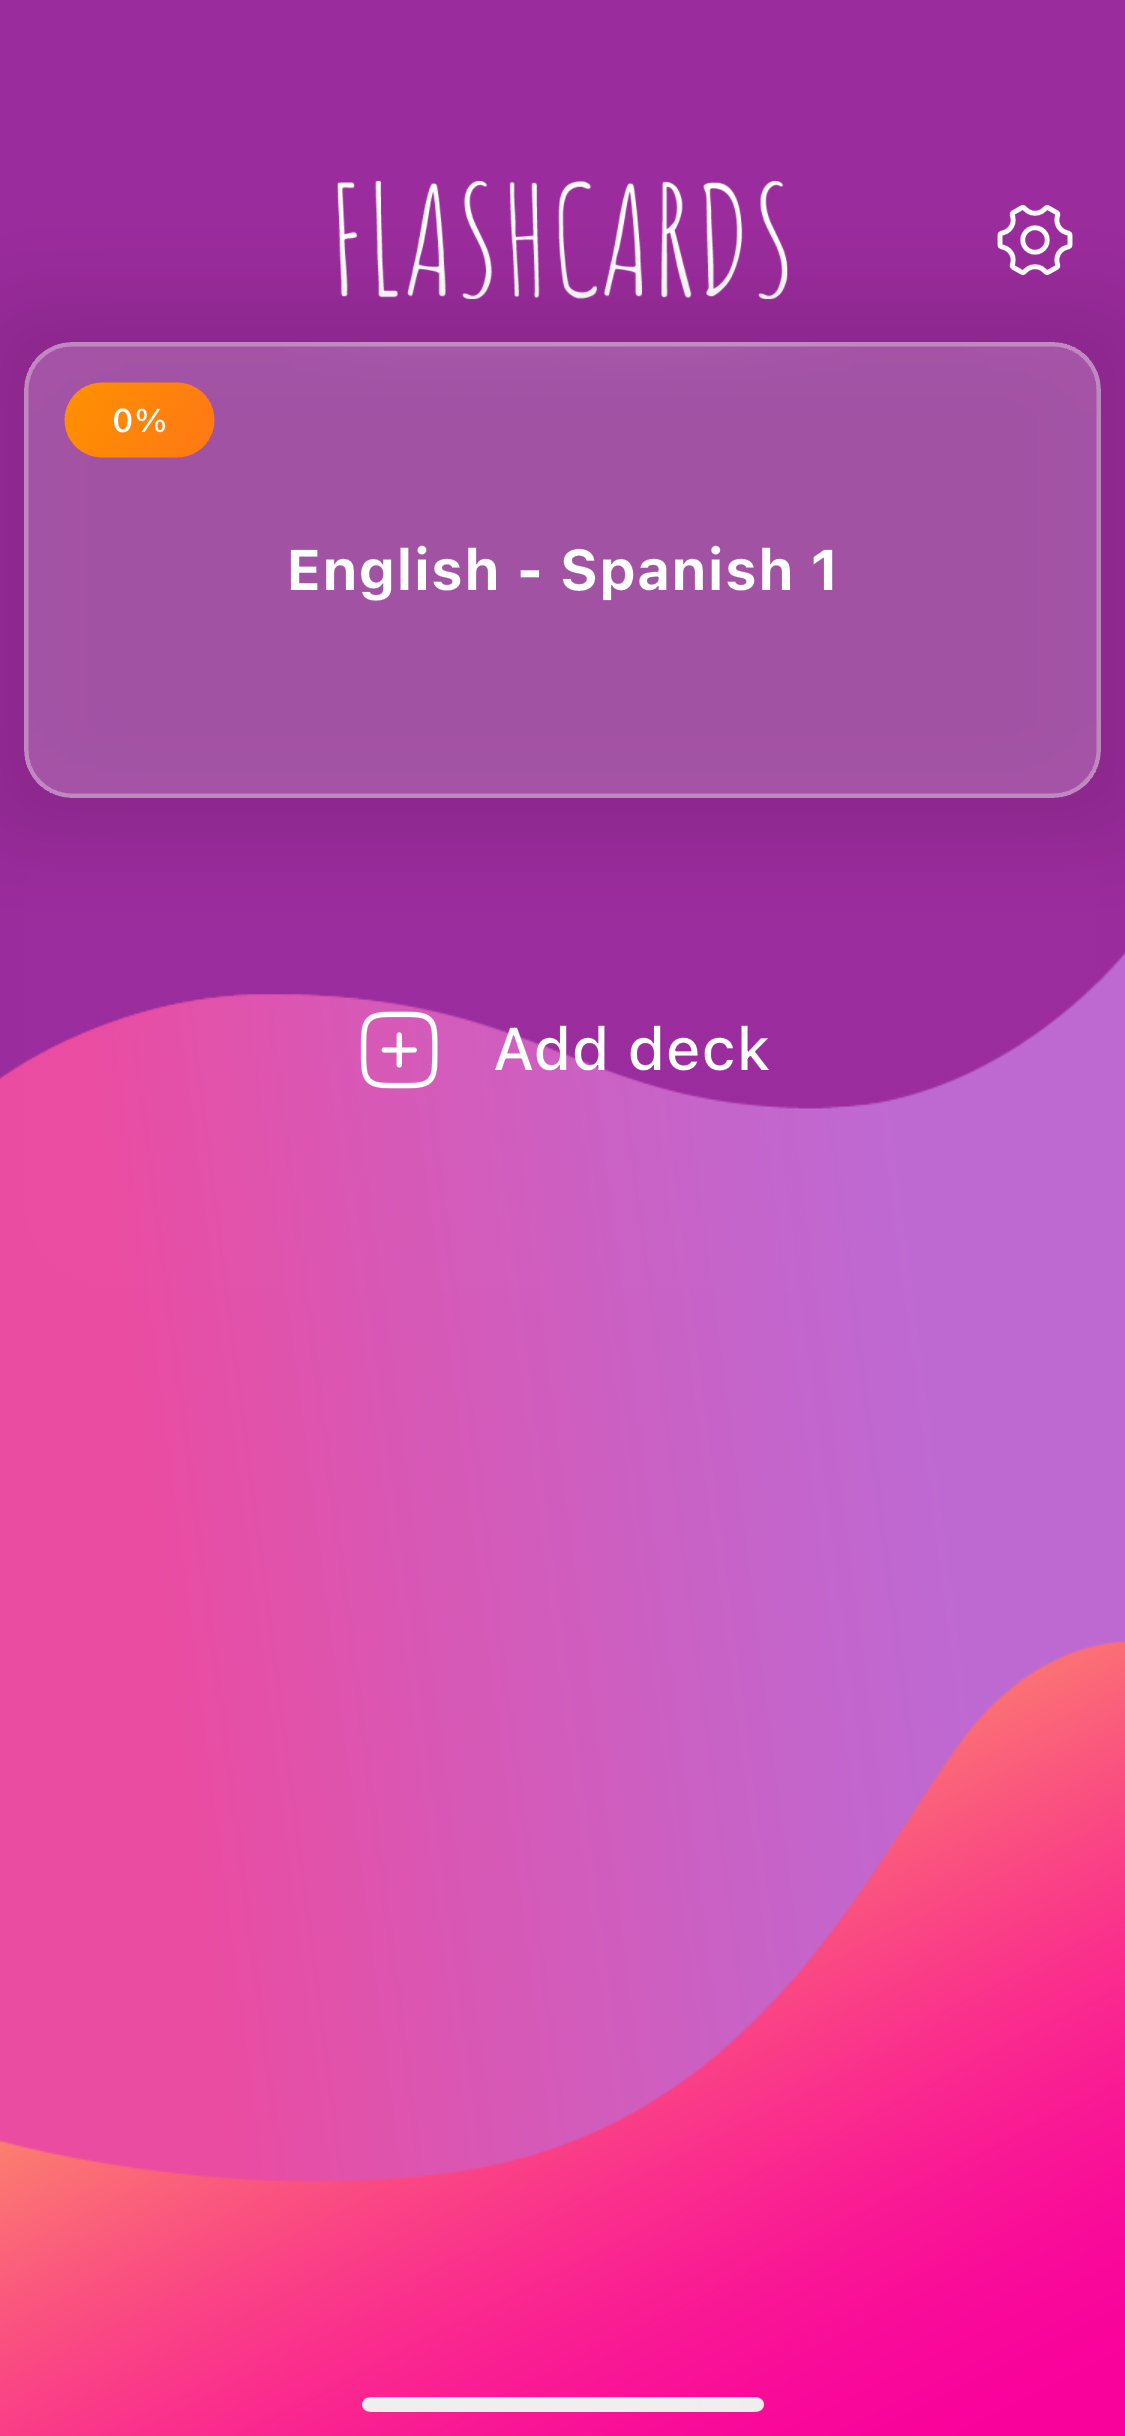
\includegraphics[width=.75\linewidth]{img/flashcards_maker1.PNG}
  \caption{Flashcards maker: Ekran główny}
  \label{fig:flashcards_maker1}
\end{minipage}%
\begin{minipage}{0.5\textwidth}
  \centering
  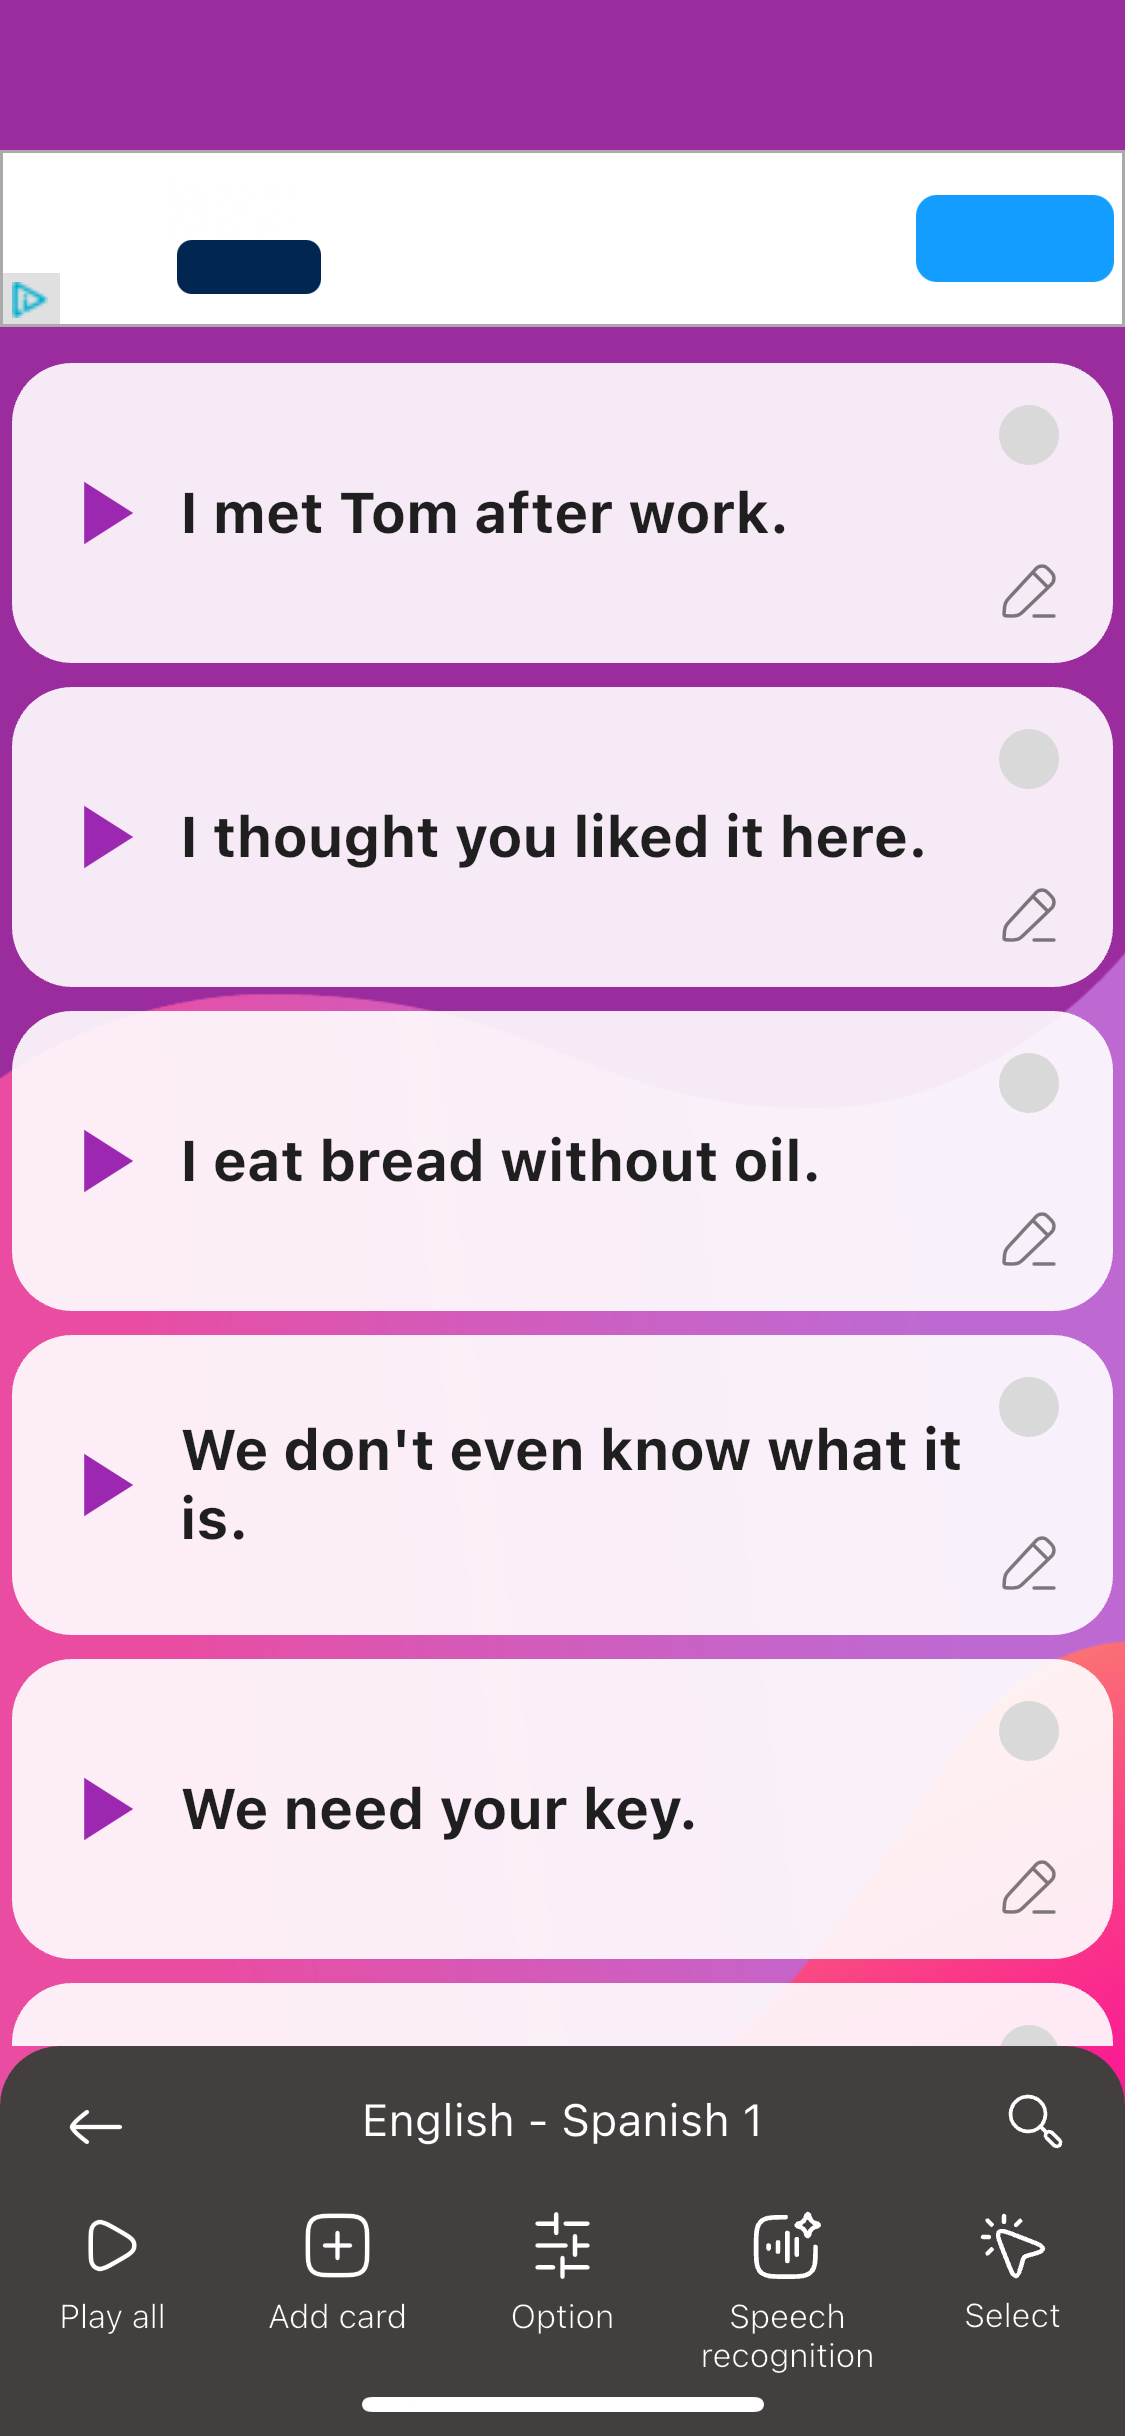
\includegraphics[width=.75\linewidth]{img/flashcards_maker2.PNG}
  \caption{Flashcards maker: Widok przykładowego zestawu fiszek}
  \label{fig:flashcards_maker2}
\end{minipage}
\end{figure}

\chapter{Zastosowane technologie}

\section{Xcode}

Środowiskiem programistycznym wybranym do zarządzania projektem jest Xcode \cite{apple_xcode}, czyli zestaw narzędzi deweloperskich do tworzenia aplikacji na platformy Apple. W ich skład wchodzi edytor kodu wewnątrz którego można kompilować, uruchamiać oraz debugować rozwijane aplikacje. Częścią oprogramowania Xcode jest również Simulator umożliwiający testowanie aplikacji na różnych urządzeniach Apple, takich jak iPhone, iPad lub AppleWatch bez potrzeby korzystania ich fizycznych odpowiedników. Xcode nie ma obecnie konkurencji na rynku --- wybór tego zestawu narzędzi jest oczywisty, ponieważ jako jedyny pozwala na stworzenie aplikacji mobilnej na system iOS. 


\section{Git}

Git \cite{git_book} to system kontroli wersji umożliwiający śledzenie zmian w kodzie źródłowym, oraz współprace zespołową przy projektach programistycznych. Jedną z jego głównych funkcji jest zapisywanie kodu źródłowego w etapach, nazywanych tutaj commit-ami. Istnieje także możliwość rozłączania oprogramowania na gałęzie, na których rozwijane są różne funkcjonalności, z możliwością późniejszego ich połączenia z powrotem do głównej gałęzi. Dzięki systemowi Git można także przywrócić dany projekt do swojej poprzedniej wersji, albo mieć ogólny wgląd w jego historię. Podczas prac nad aplikacją mobilną będącą tematem aplikacji, Git zastosowany został w celu zachowania historii zmian.


\section{Swift}

Swift \cite{swift_apple_developer} jest językiem programowania stworzonym przez firmę Apple. Głównym celem jego kreacji było zastąpienie Objective-C jako języka używanego podczas tworzenia oprogramowania na platformy Apple. Jest to wysokopoziomowy, kompilowany język zawierający nowoczesne funkcje, takie jak inferencja typów, która ułatwia pisanie kodu oraz zmniejsza szanse na wystąpienie potencjalnych błędów. Język Swift nie wymaga pisania średników na końcach linijek a jego system modułów eliminuje potrzebę tworzenia plików nagłówkowych. Dodatkowo kodowanie ciągów znaków w tym języku bazowane jest na UTF-8, co ułatwia korzystanie ze znaków specjalnych w aplikacji. Pamięć w Swift jest zarządzana poprzez system ARC (ang. Automatic Reference Counting), który automatycznie usuwa niewykorzystywane zasoby z pamięci.


\section{SwiftUI}

SwiftUI \cite{swiftui_xcode} jest biblioteką rozwijaną przez firmę Apple zajmującą się tworzeniem interfejsów użytkownika, Jej zadaniem jest zastąpić bibliotekę UIKit, która do 2019 roku była głównym sposobem na tworzenie aplikacji na systemy iOS oraz iPadOS. Jednak cały czas jest w trakcie rozwoju co sprawia, że UIKit nadal utrzymuje się jako dominująca technologia w tej dziedzinie. 

Tworzenie interfejsów za pomocą SwiftUI \cite{apple_swiftui} ma charakter deklaratywny --- analogiczny do innych technologii internetowych, takich jak na przykład React. Oznacza to, że deweloper w trakcie tworzenia wyglądu aplikacji opisuje to co ma się na ekranie wyświetlić, a nie w jaki sposób. Dzięki temu przy rozwoju interfejsu użytkownika występuje automatyczna synchronizacja widoku z danymi. 

W środowisku SwiftUI każdy element graficzny interfejsu użytkownika musi implementować protokół \texttt{View} (tłum. widok). Z tego względu w tej pracy wszystkie komponenty wizualne aplikacji będą określane mianem widoków.

Makra zapewniają reaktywność z minimalną dodatkową konfiguracją: \texttt{@State} pozwala na przechowywanie zmiennej lokalnej, na której zmianę interfejs będzie reagował automatycznie, \texttt{@Binding} pozwala widokowi na otrzymanie dostępu do zmiennej wraz z możliwością jej modyfikacji. Takie podejście jest często stosowane przy polach tekstowych. 

Kolejnym przydatnym makrem jest \texttt{@Observable} używane w celu wyodrębniania stanu aplikacji. Pozwala ono na utworzenie obiektu, który będzie automatycznie śledził zmiany każdych z jego atrybutów i aktualizował interfejs w przypadku ich nastąpienia. Jest to uproszczeniem w porównaniu do poprzedniego rozwiązania, gdzie taki obiekt musiałby dziedziczyć protokół \texttt{StateObject}. Ponadto każdy z jego atrybutów musiałby zostać oznaczony makrem \texttt{@Published}, by interfejs reagował na ich zmiany. Rozwiązanie to mniej efektywnie wykorzystuje zasoby systemu, ponieważ jednego parametru wywoływała ponowne renderowanie każdego elementu interfejsu korzystającego z tego obiektu. Natomiast używając makra \texttt{@Observable} renderowane są tylko te części interfejsu, gdzie faktycznie nastąpiła jakaś zmiana.



\section{SwiftData}

SwiftData to biblioteka udostępniona przez firmę Apple umożliwiająca modelowanie danych przechowywanych wewnątrz aplikacji. Architektura opiera się o wcześniejszą bibliotekę Apple spełniającą tą rolę: Core Data, która była wrapperem ORM wokół bazy danych SQLite. Główną zaletą Core Data była jej skuteczna integracja z istniejącymi w Objective-C typami. Mimo że istnieje możliwość użycia jej podczas budowania aplikacji w języku Swift, nie wspiera ona wielu nowoczesnych funkcji językowych, takich jak na przykład wsparcie generyków. Z tego powodu biblioteką użytą w trakcie pracy został pakiet SwiftData.


\chapter{Diagramy UML}

\section{Diagram przypadków użycia}

\begin{figure}[h]
    \centering
    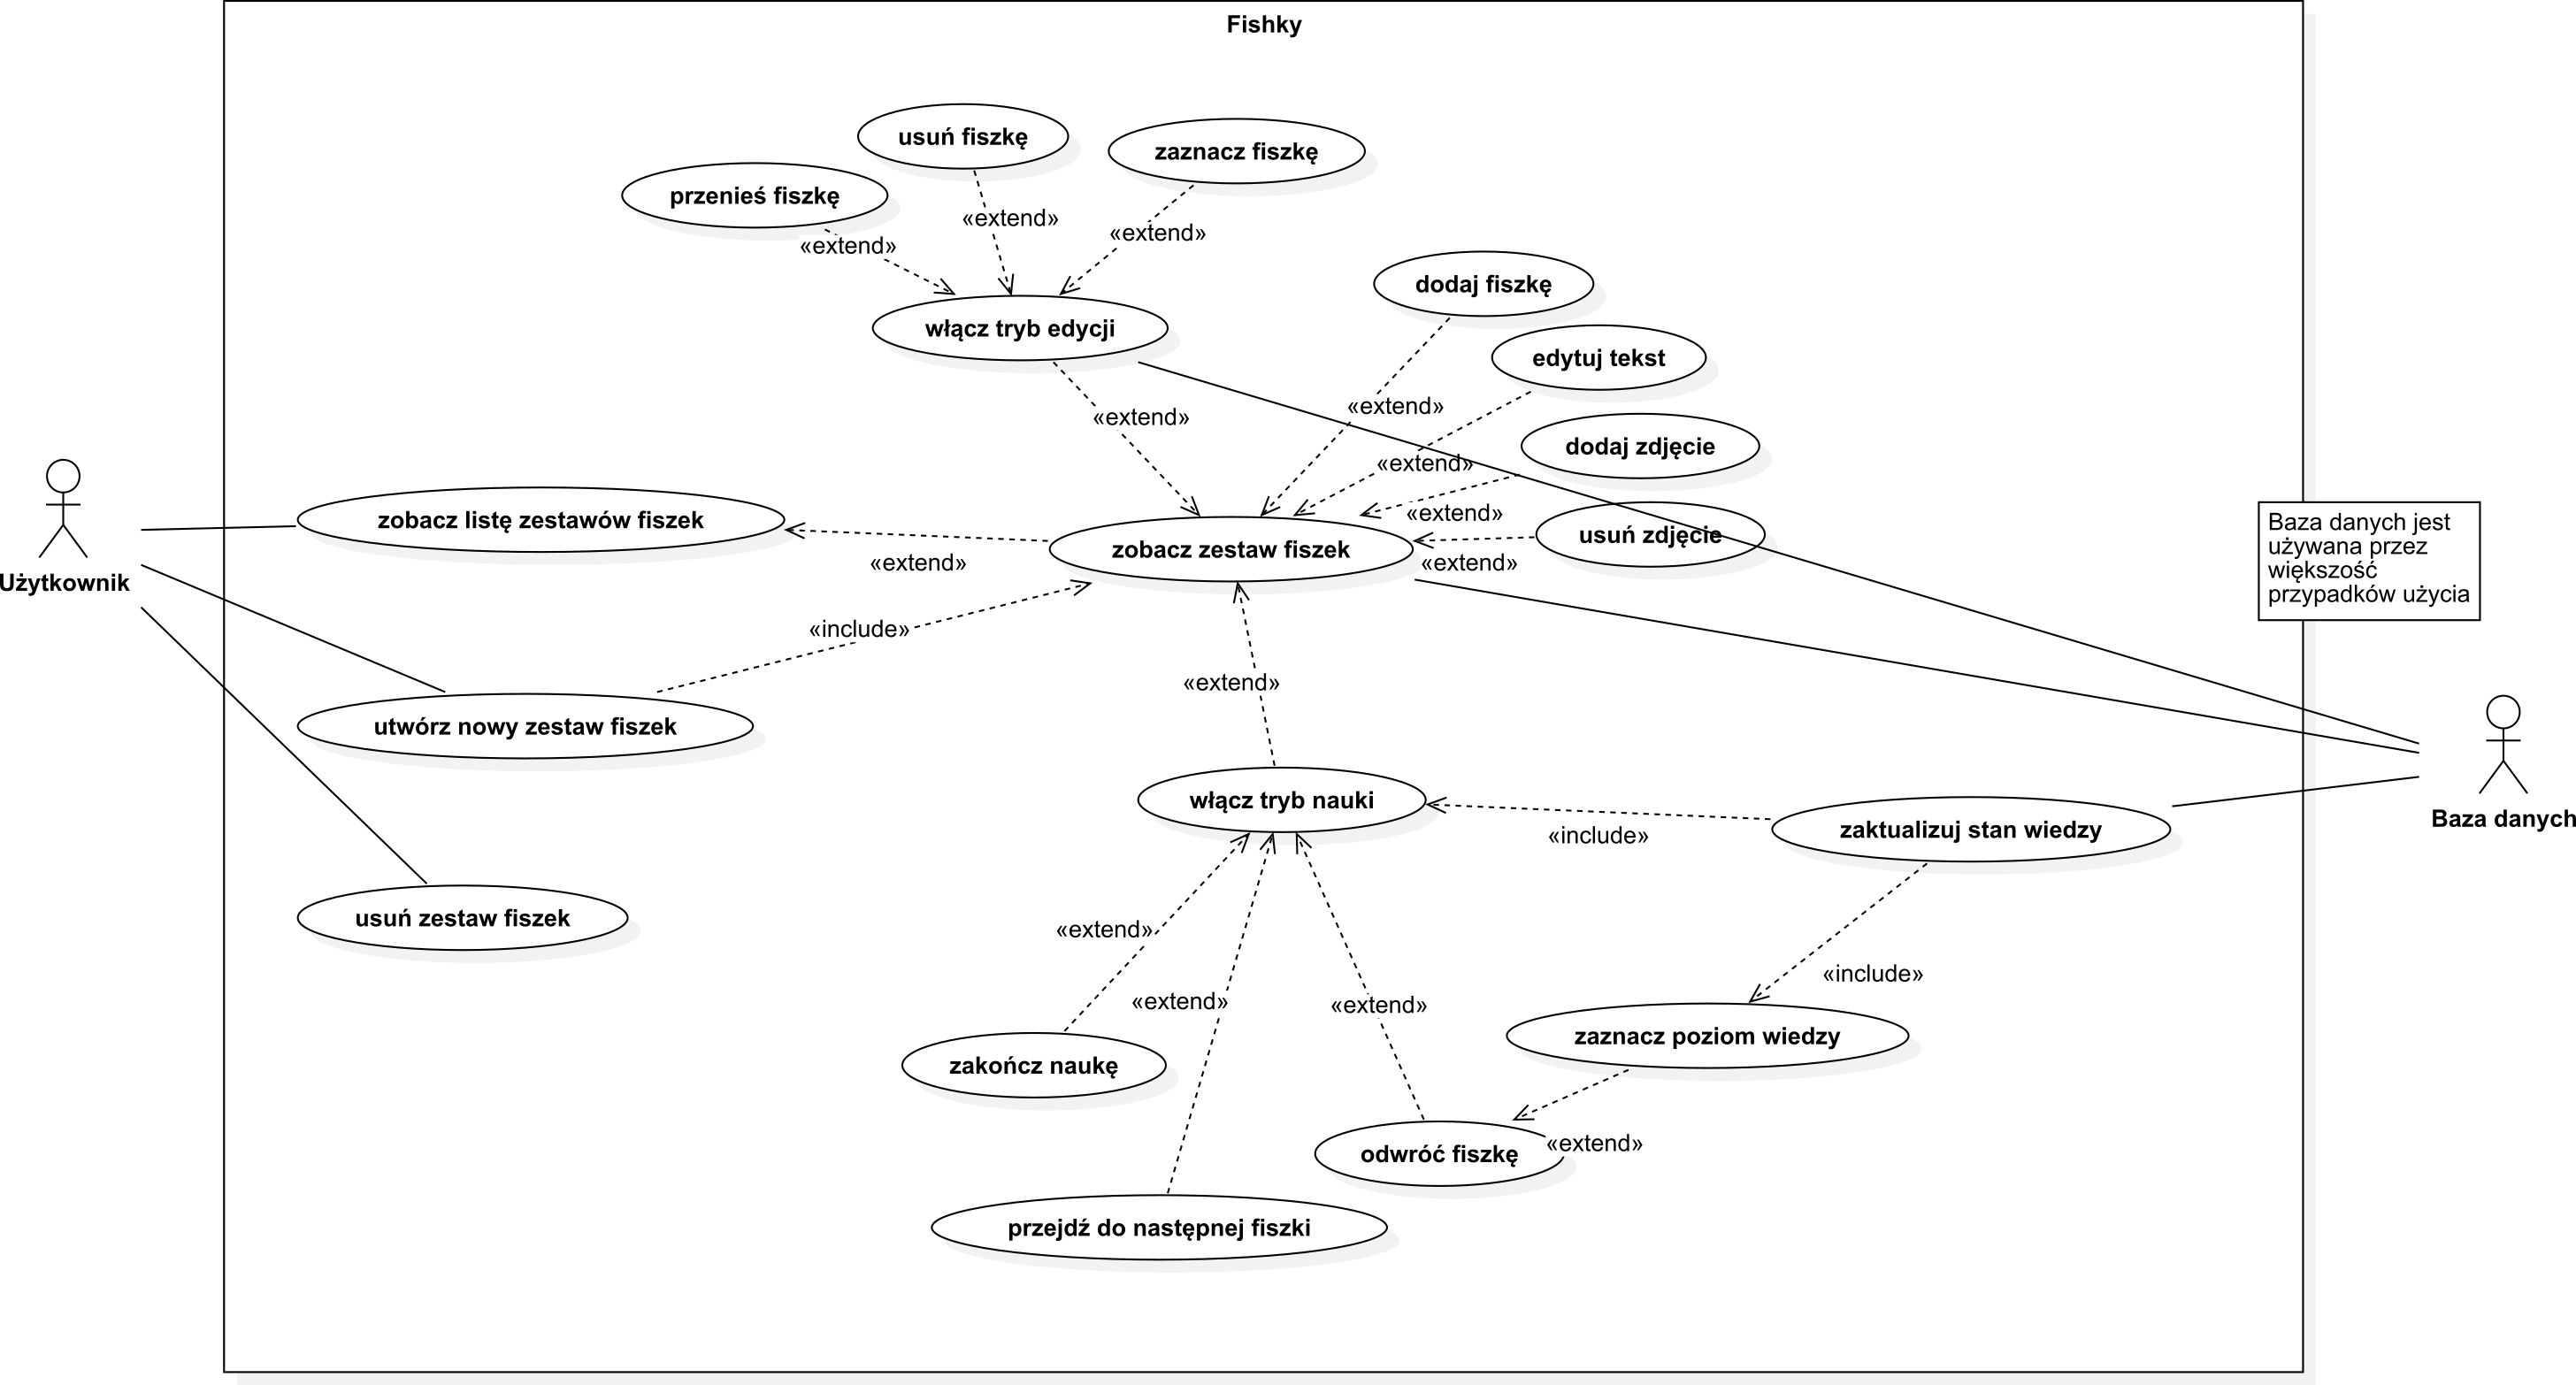
\includegraphics[width=1.0\textwidth]{img/UseCaseDiagram1.png}
    \caption{Diagram przypadków użycia}
    \label{fig:UseCaseDiagram1}
\end{figure}

\section{Diagram klas}

\begin{figure}[H]
    \centering
    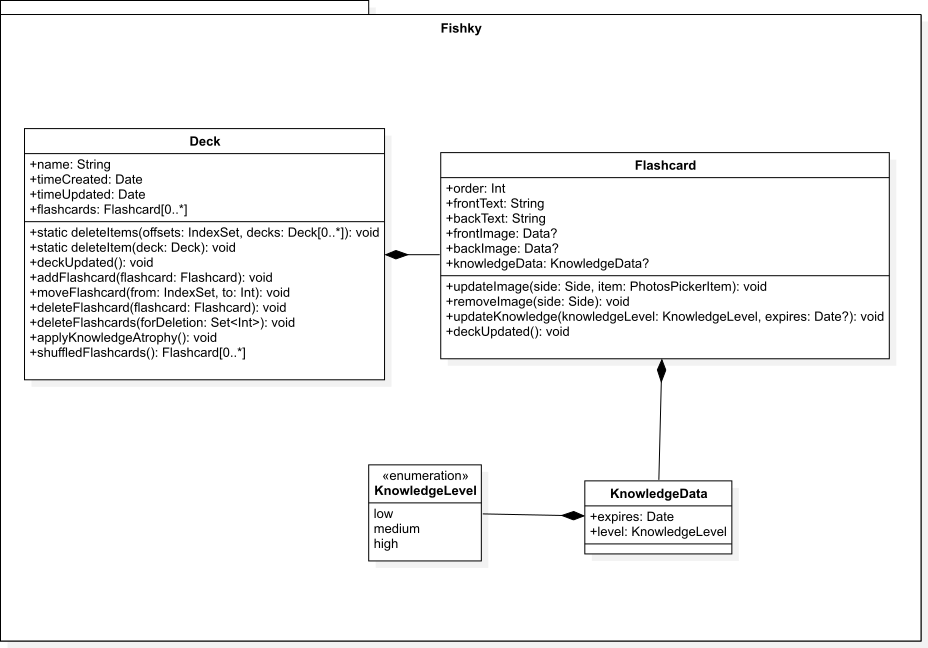
\includegraphics[width=1.0\textwidth]{img/ClassDiagram1.png}
    \caption{Diagram klas}
    \label{fig:ClassDiagram1}
\end{figure}


\chapter{Struktura aplikacji}

\section{Ekran startowy}

\begin{figure}[H]
\centering
\begin{minipage}{0.5\textwidth}
  \centering
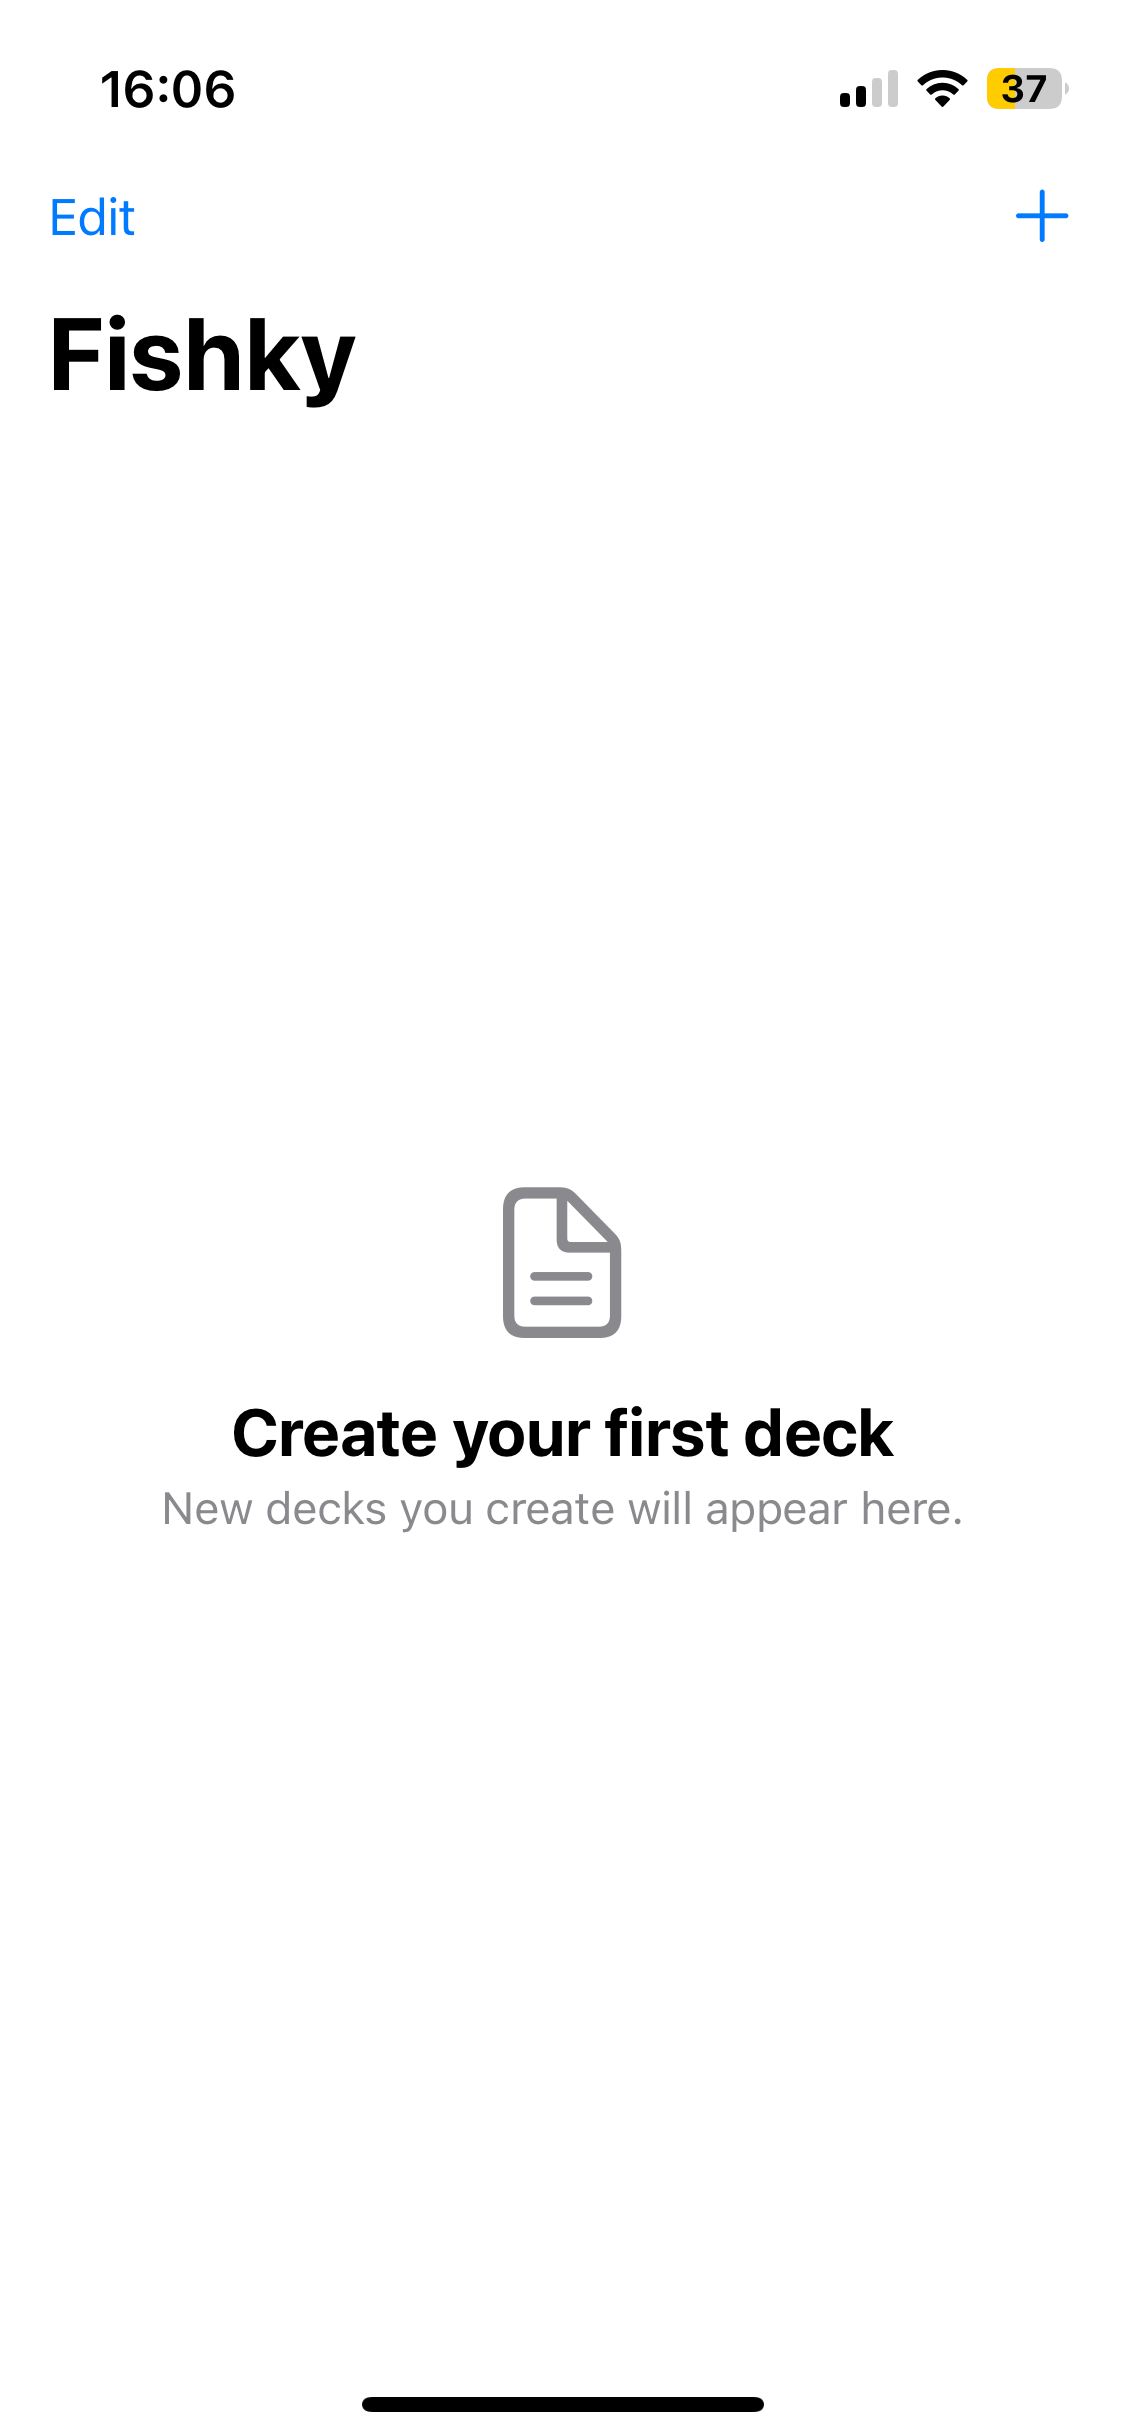
\includegraphics[width=.75\linewidth]{img/fishky1.PNG}
  \caption{Ekran startowy bez żadnych zestawów fiszek}
  \label{fig:fishky1}
\end{minipage}%
\begin{minipage}{0.5\textwidth}
  \centering
  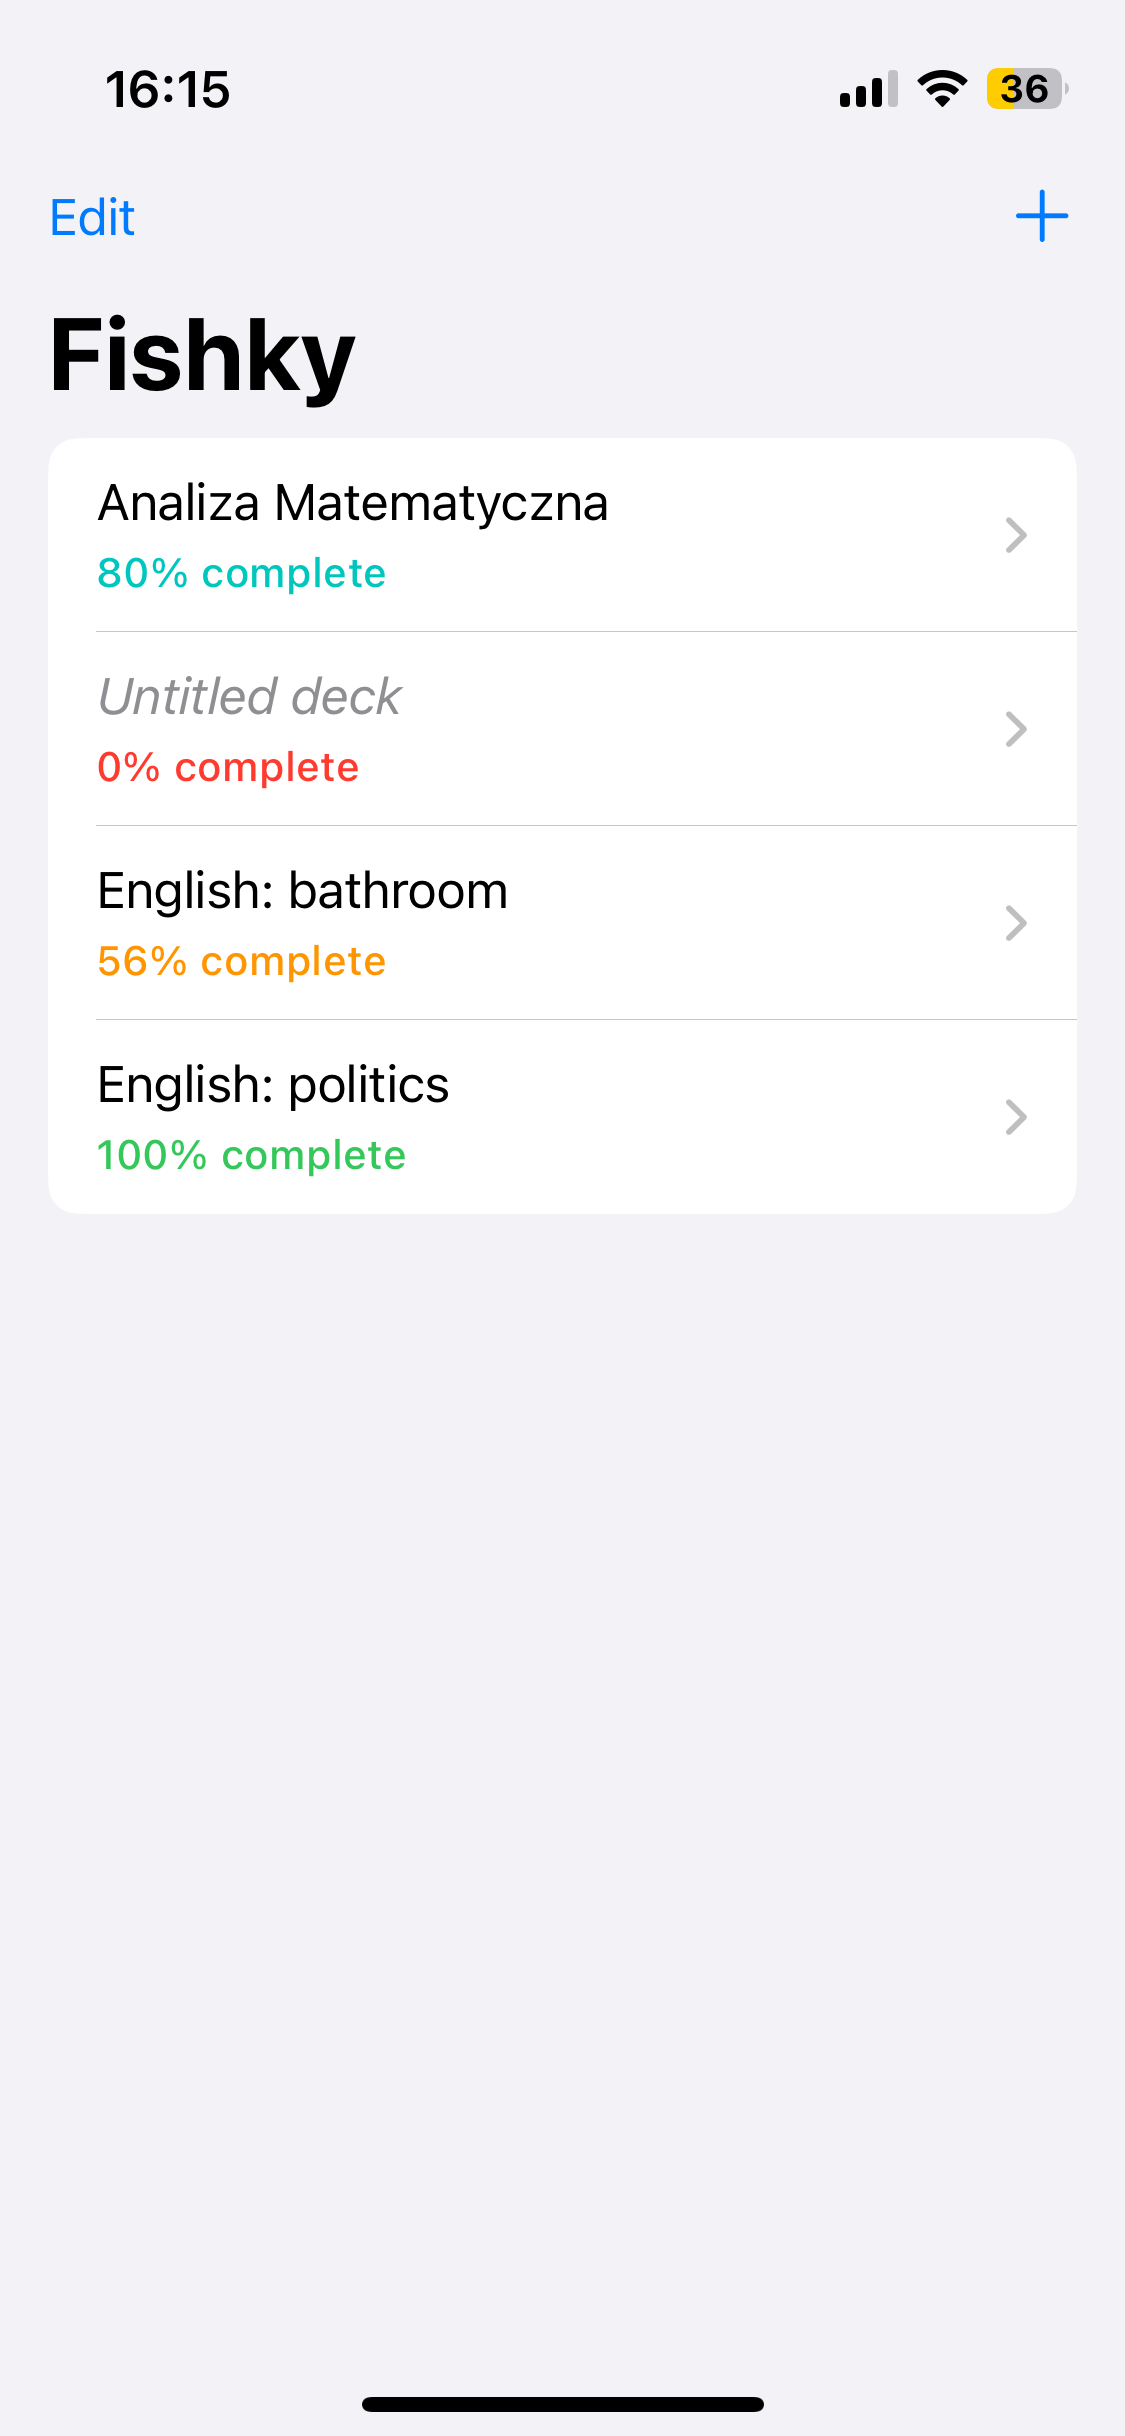
\includegraphics[width=.75\linewidth]{img/fishky2.PNG}
  \caption{Ekran startowy z zestawami fiszek}
  \label{fig:fishky2}
\end{minipage}
\end{figure}

Otwierając aplikacje użytkownik widzi ekran główny będący listą zestawów fiszek. W przypadku, gdy jest to pierwsze uruchomienie programu na środku ekranu znajduje się napis informujący go o tym, że w tym miejscu pojawią się utworzone przez użytkownika zestawy. Każdy zestaw na liście posiada swój poziom nauczenia, czyli procent obliczany na podstawie tego na ile fiszek użytkownik udzielił poprawnych odpowiedzi. Poziomy oznaczone są różnymi kolorami: od czerwonego, który oznacza zerowy procent wiedzy do zielonego, który informuje użytkownika o przekroczeniu progu 95 procent. 

W górnej części aplikacji widnieje jej tytuł a tuż nad nim na pasku narzędzi znajduje się guzik ,,Edit'', którego funkcją jest włączenie trybu edycji. Po drugiej stronie, w prawym górnym rogu ekranu znaleźć można guzik z ikoną plus umożliwiający dodanie nowego zestawu fiszek.


\section{Ekran edycji zestawu fiszek}

\begin{figure}[h]
\centering
\begin{minipage}{0.5\textwidth}
  \centering
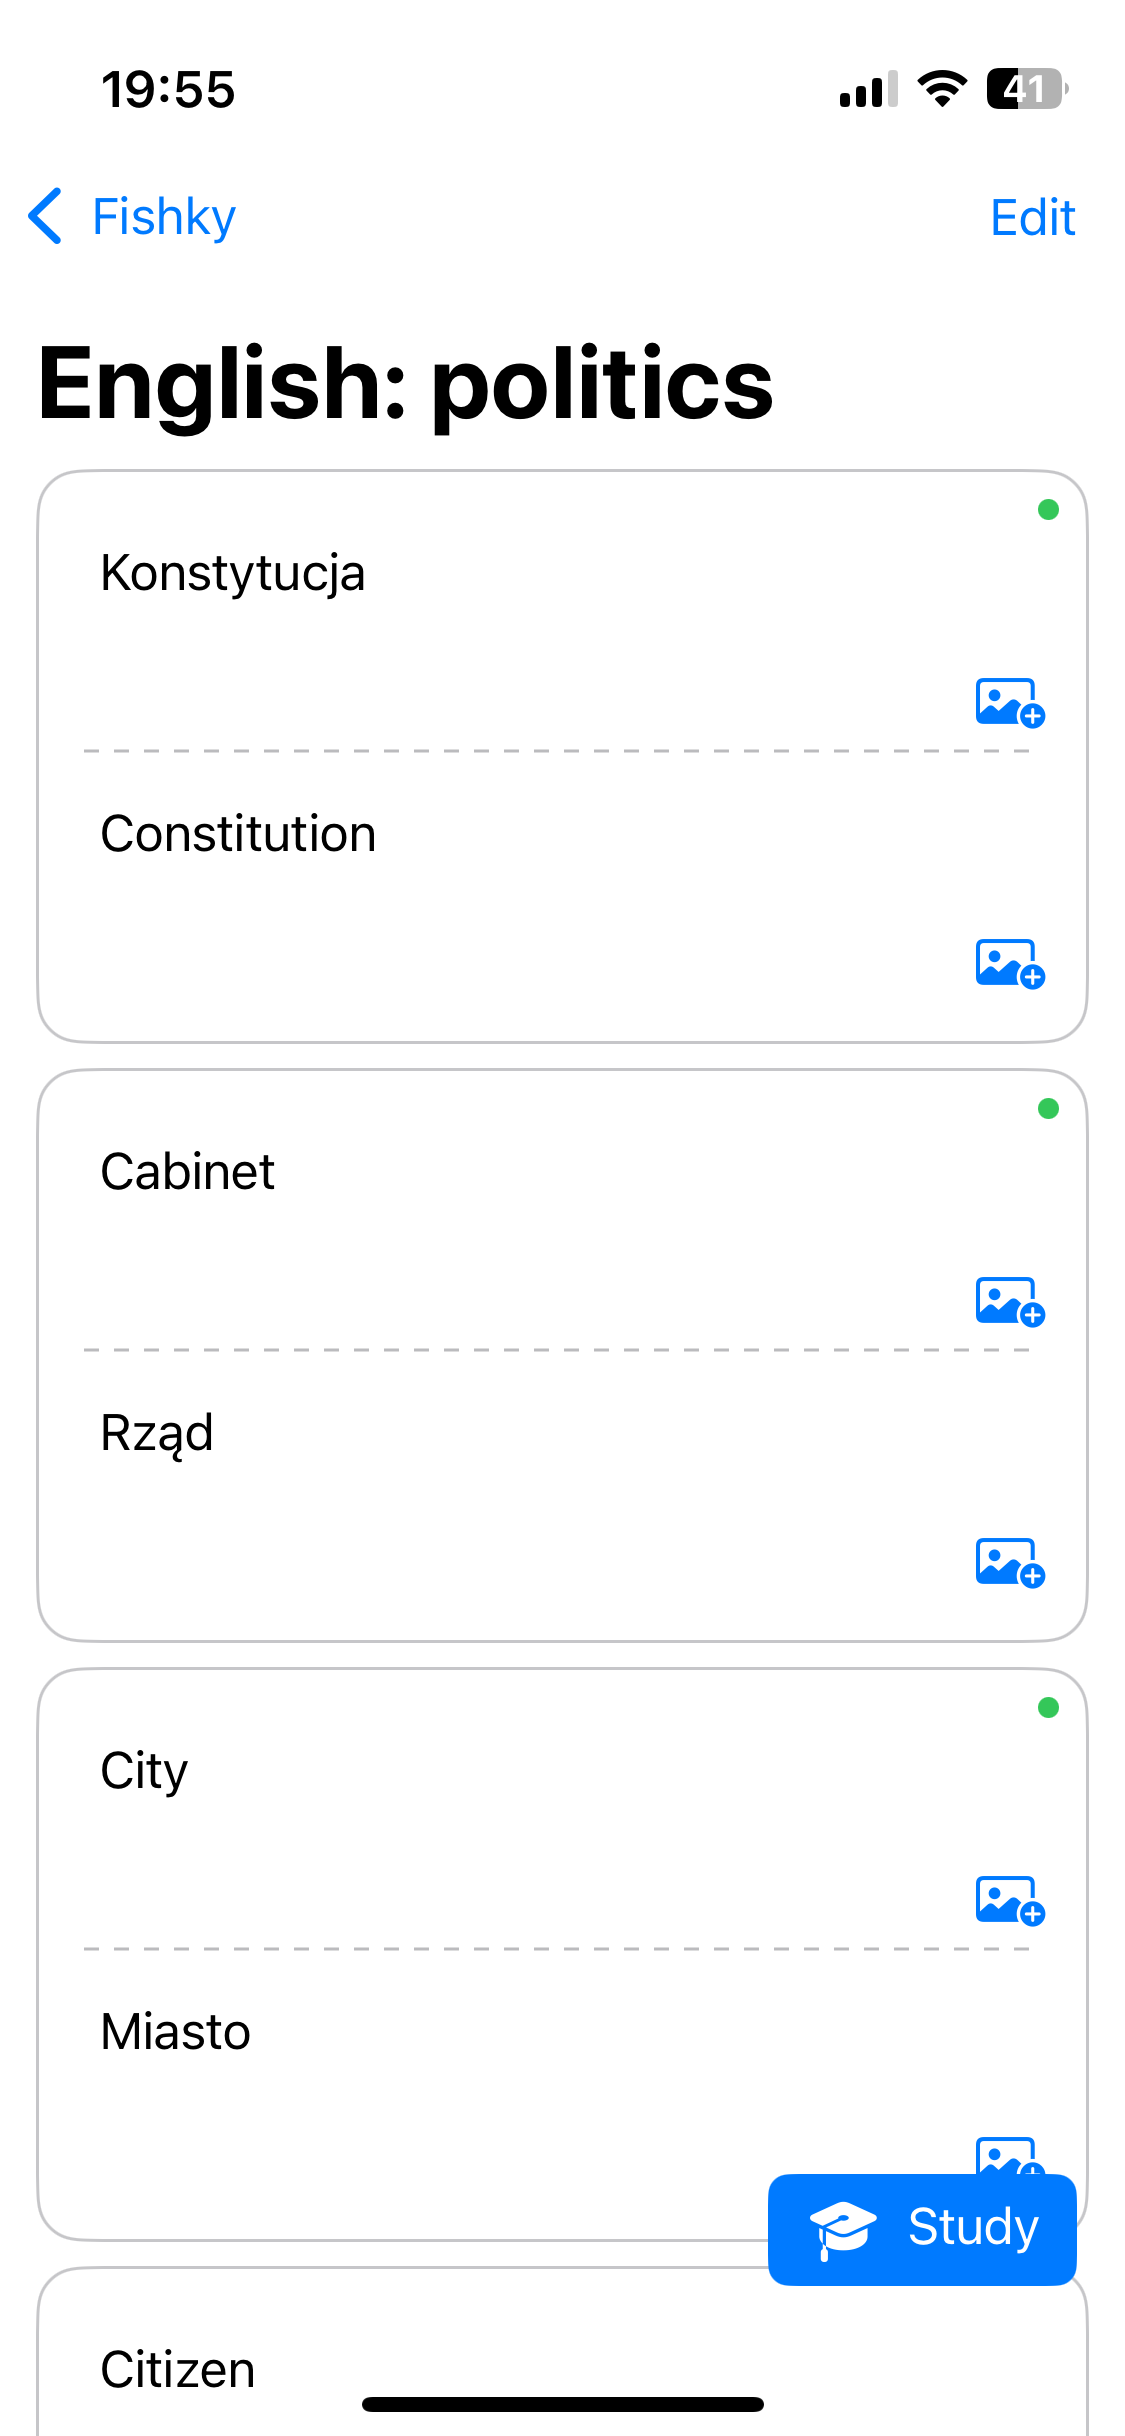
\includegraphics[width=.75\linewidth]{img/fishky3.PNG}
  \caption{Zestaw fiszek}
  \label{fig:fishky3}
\end{minipage}%
\begin{minipage}{0.5\textwidth}
  \centering
  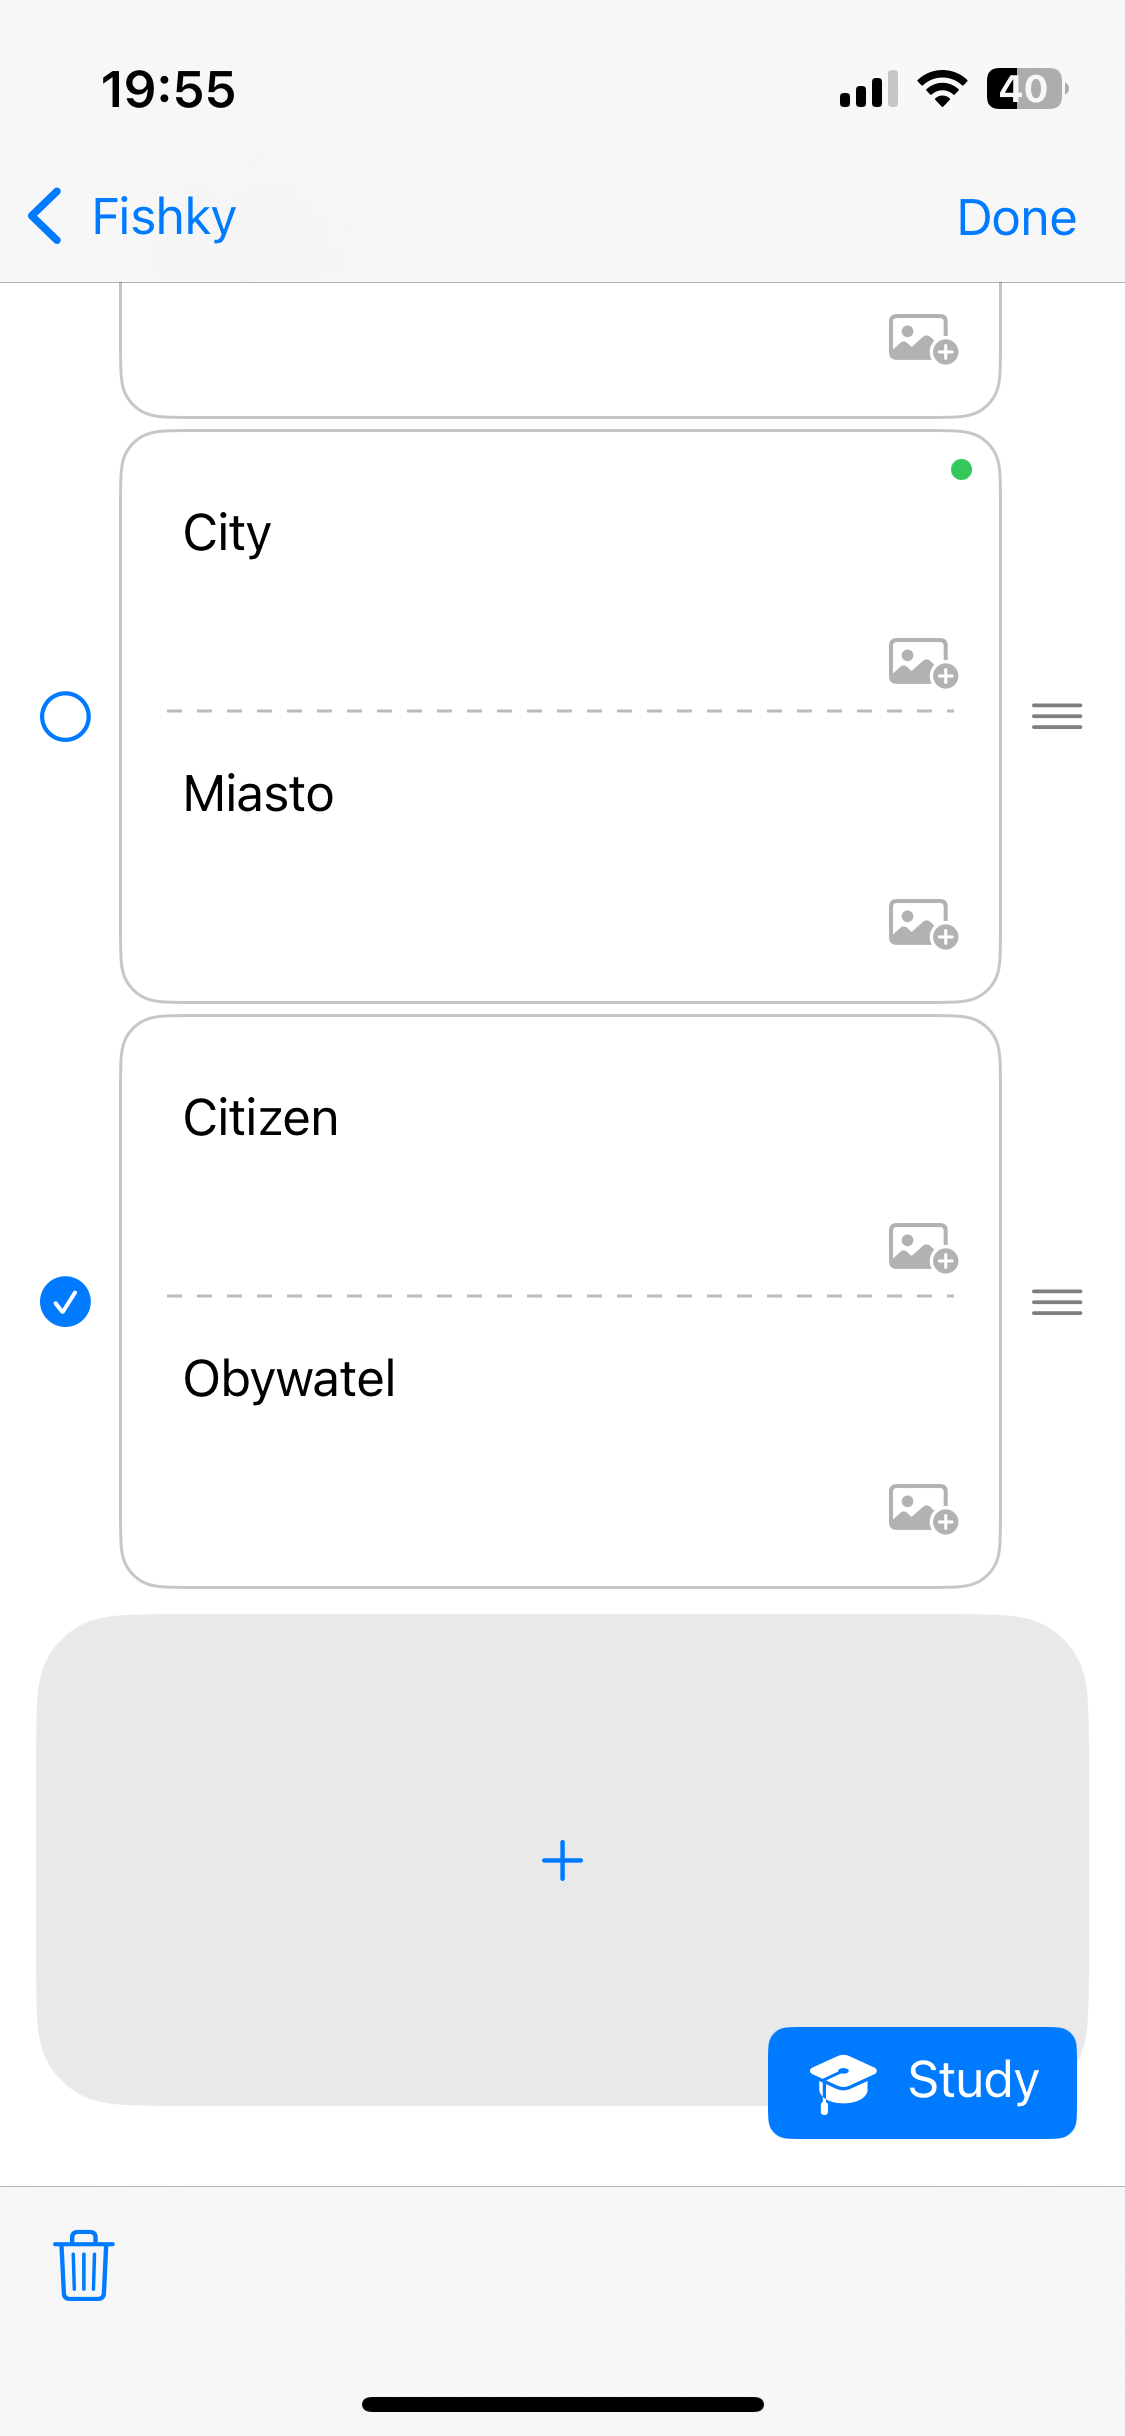
\includegraphics[width=.75\linewidth]{img/fishky4.PNG}
  \caption{Zestaw fiszek w trybie edycji}
  \label{fig:fishky4}
\end{minipage}
\end{figure}

Po utworzeniu nowego zestawu fiszek użytkownik jest przekierowywany na stronę jego edycji. Na samej górze znajduje się pasek narzędzi, po którego lewej stronie widoczny jest, zgodnie z konwencjami znanymi w systemie iOS, guzik cofania umożliwiający przejście do poprzedniego ekranu. Po drugiej stronie paska znajduje się przycisk po naciśnięciu, którego włącza się tryb edycji fiszek. Domyślną nazwą zestawu jest ,,Untitled deck'' oznaczona szarym kolorem. Po kliknięciu na nią użytkownik ma możliwość zmiany tytułu, który przybiera wtedy kolor czarny. Poniżej nazwy znajduje się szary guzik z ikoną plusa, który udostępnia funkcję dodania nowej fiszki do danego zestawu. W prawym dolnym rogu ekranu znajduje się także niebieski przycisk do aktywacji trybu nauki.

Każda fiszka posiada swój przód oraz tył znajdujące się na jednym kafelku. Oddzielone są przerywaną linią, by użytkownik miał możliwość jednoczesnej edycji obu stron jednocześnie. Na karcie znajdują się także dwa guziki umożliwiające dodanie zdjęcia do każdej ze stron. Po zakończeniu trybu nauki danego zestawu fiszek w prawym górnym rogu każdego kafelka pojawia się kropka, która swoim kolorem informuje użytkownika o poziomie wiedzy danej fiszki.


\section{Tryb nauki}

\begin{figure}[h]
\centering
\begin{minipage}{0.5\textwidth}
  \centering
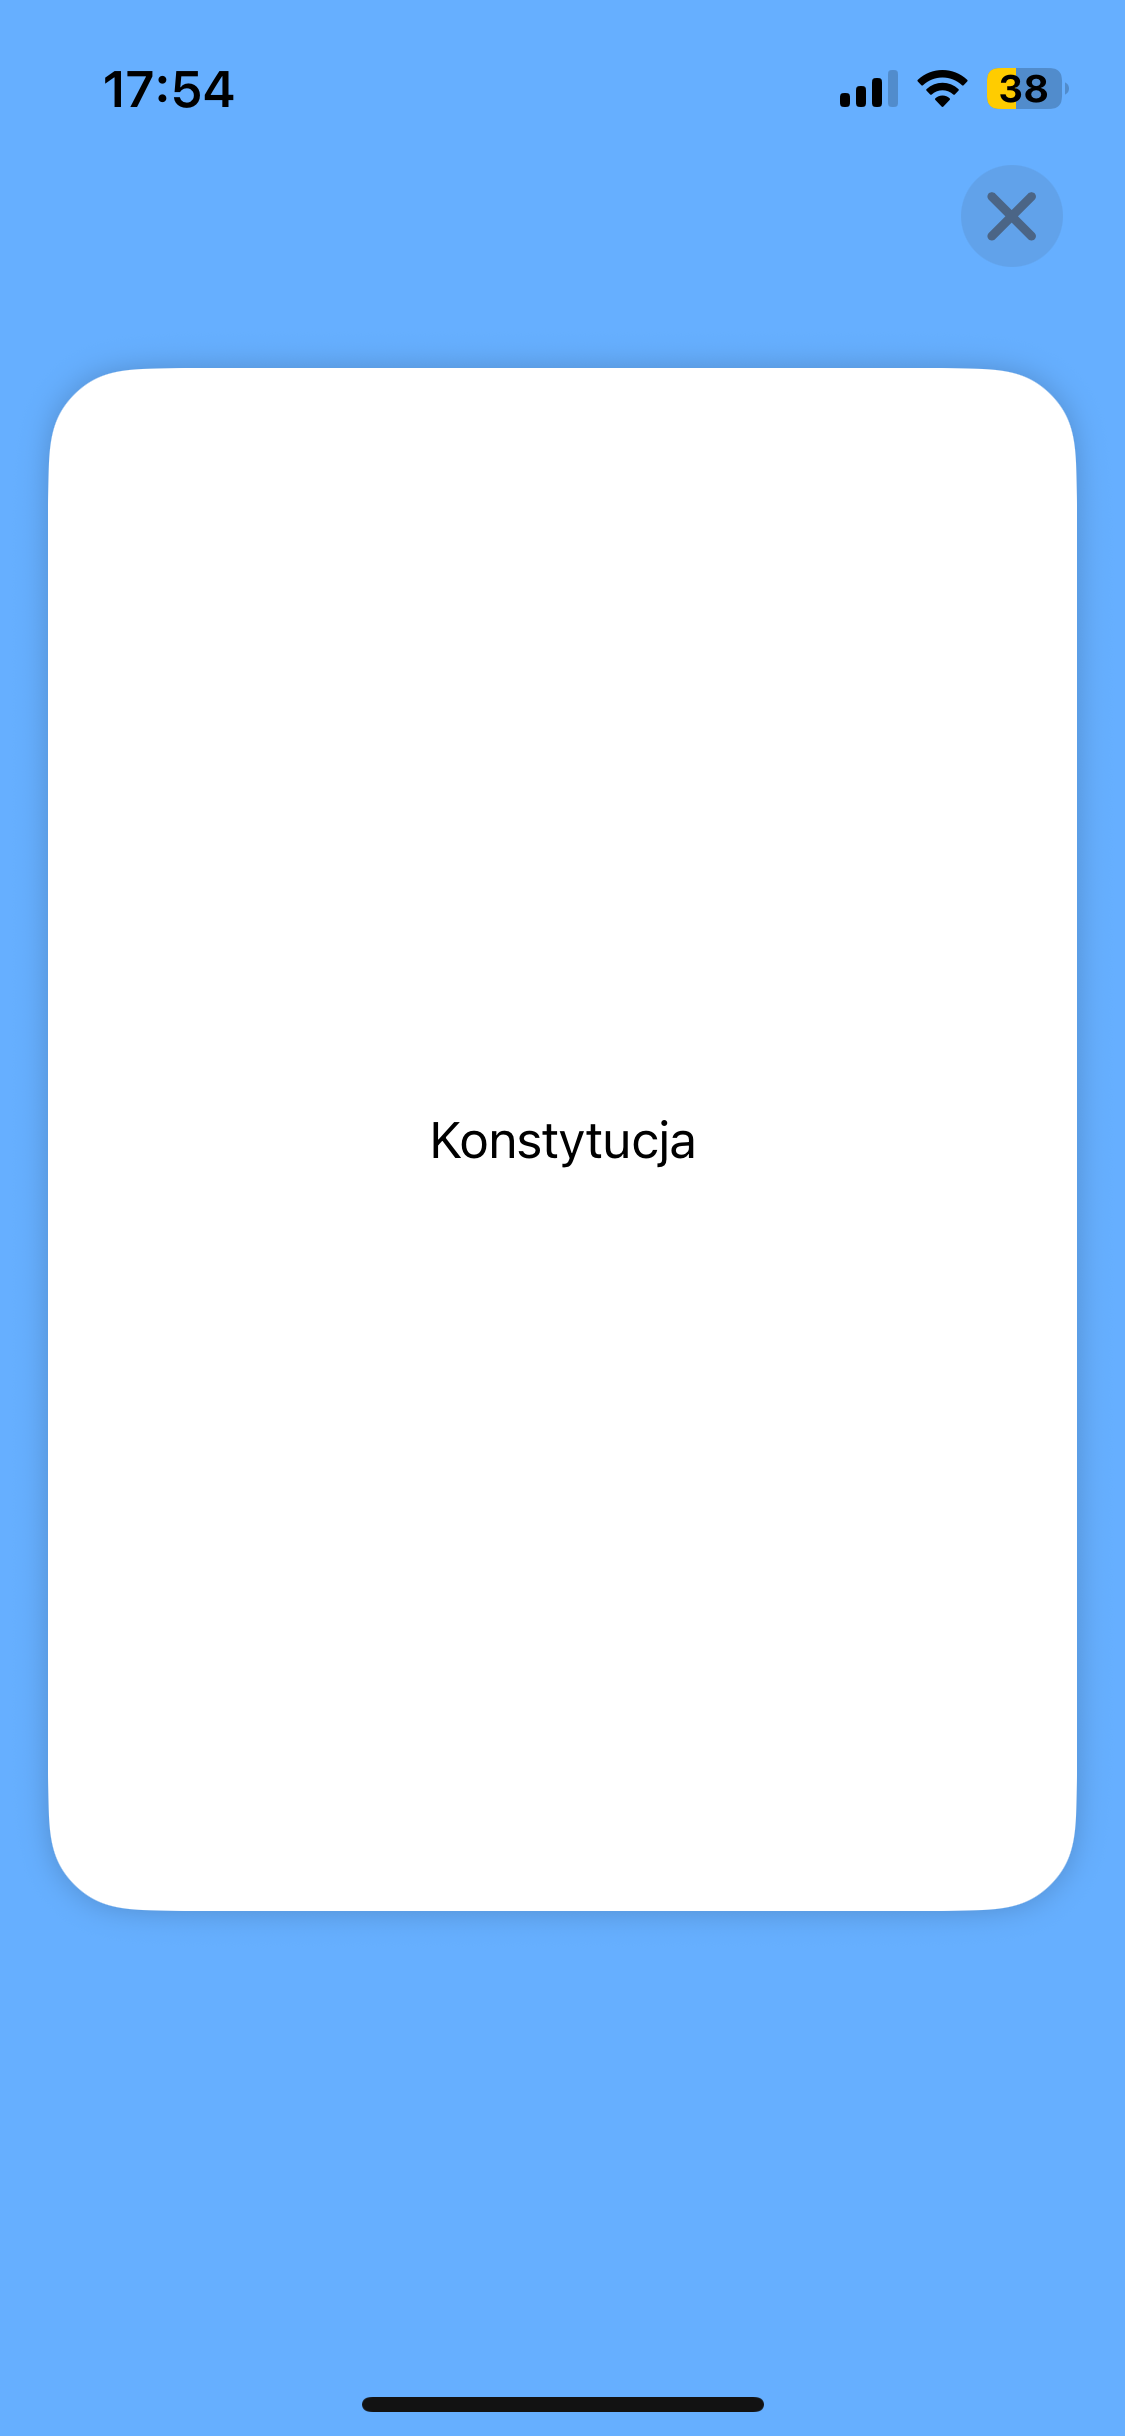
\includegraphics[width=.75\linewidth]{img/fishky5.PNG}
  \caption{Tryb nauki}
  \label{fig:fishky5}
\end{minipage}%
\begin{minipage}{0.5\textwidth}
  \centering
  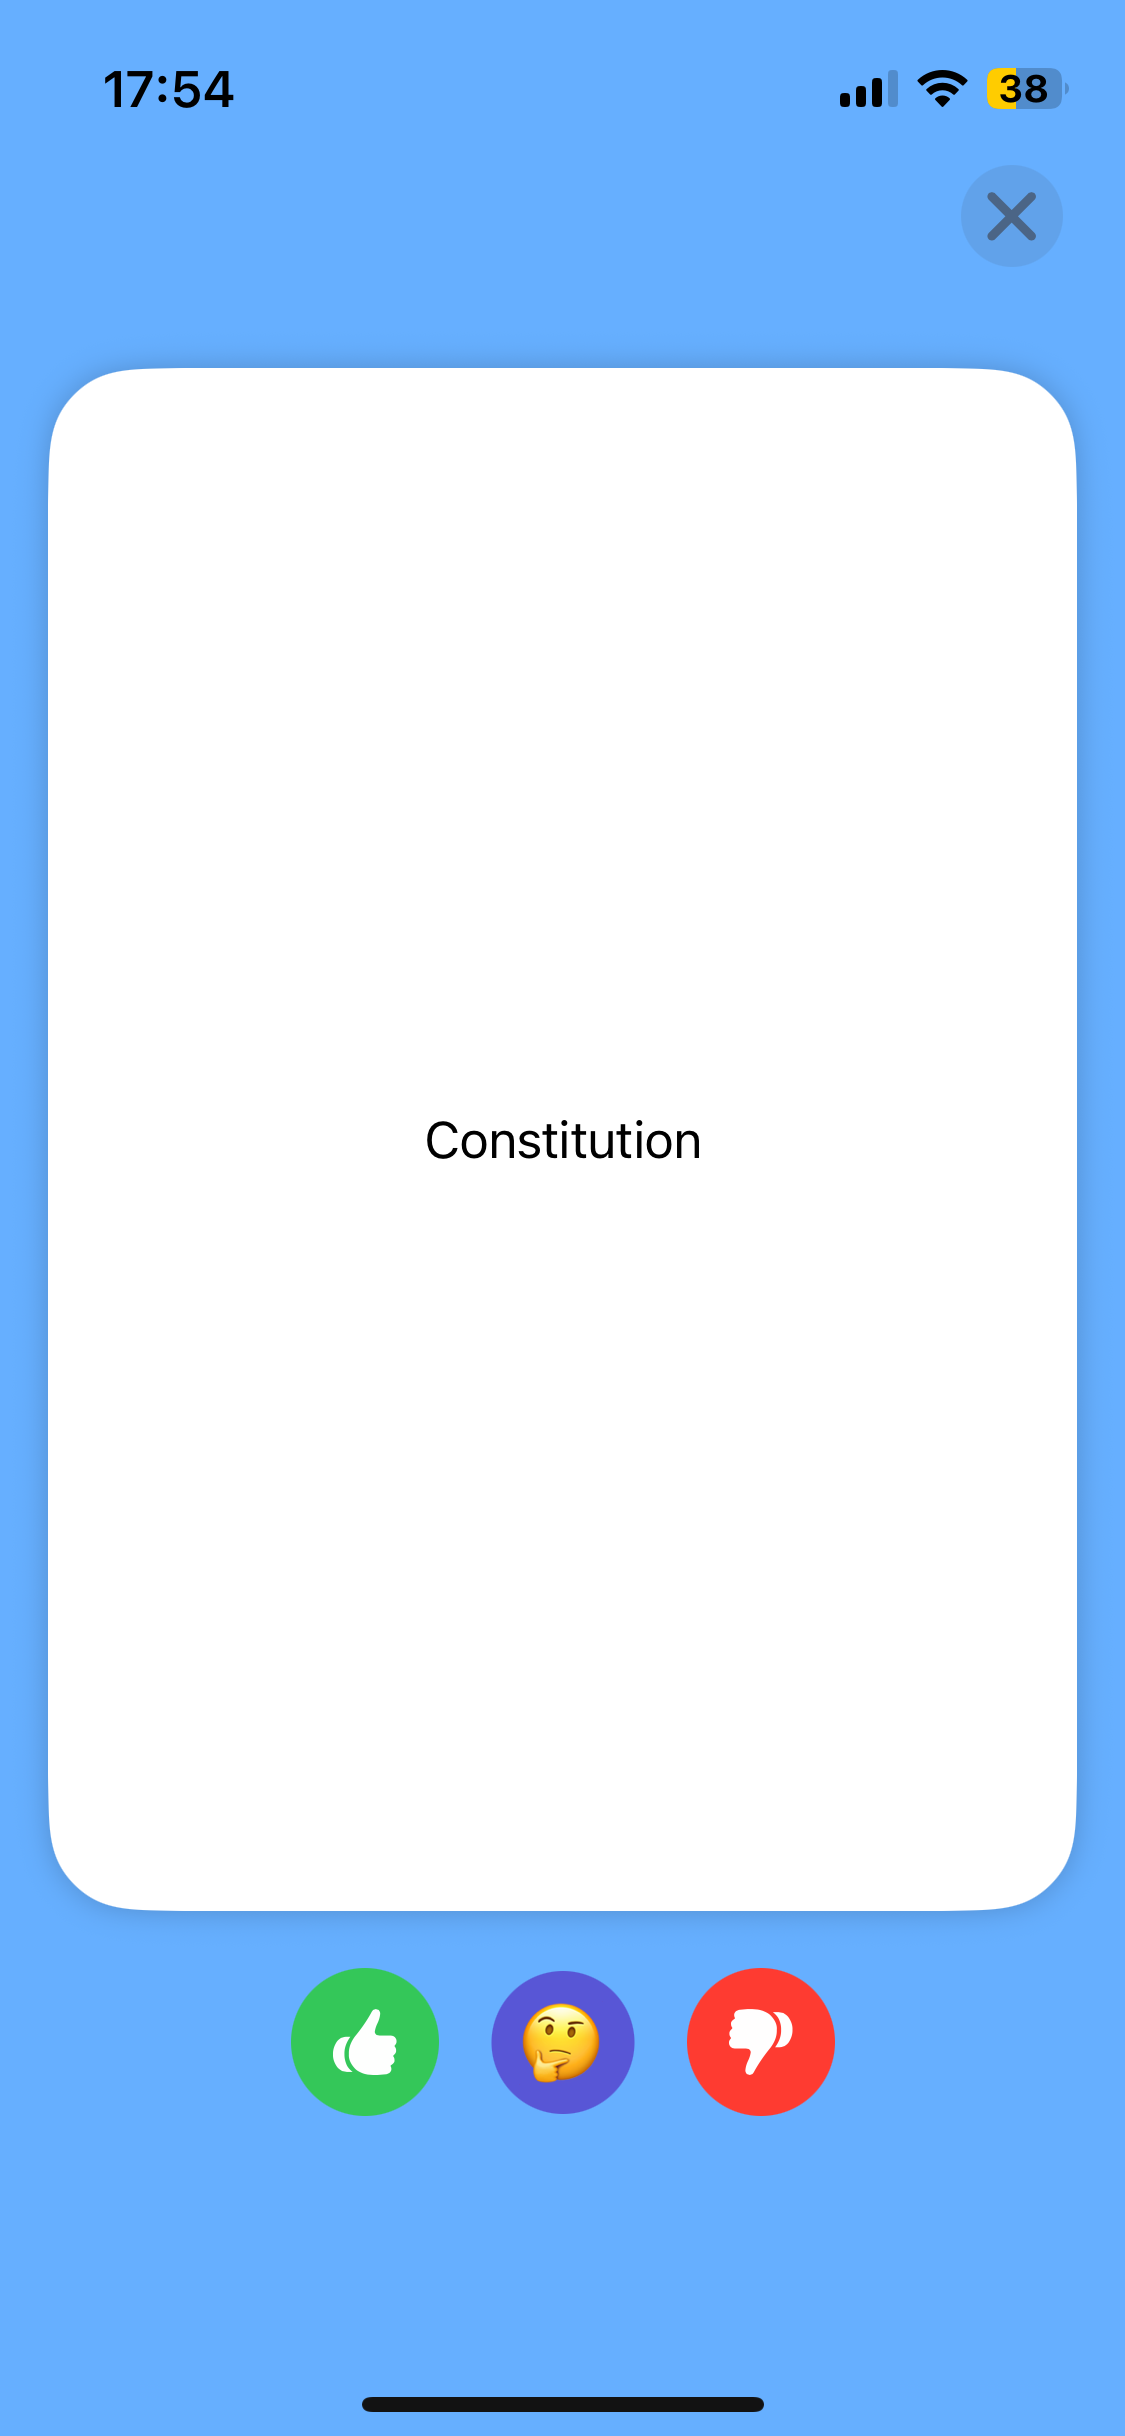
\includegraphics[width=.75\linewidth]{img/fishky6.PNG}
  \caption{Tryb nauki po odwróceniu fiszki}
  \label{fig:fishky6}
\end{minipage}
\end{figure}

Włączenie trybu nauki powoduje przejście do pełnoekranowego widoku z guzikiem umożliwiającym jego zamknięcie w prawym górnym rogu. Na środku ekranu znajduje się przednia strona fiszki zawierająca tekst wraz z opcjonalnym zdjęciem. Kliknięcie na nią powoduje rozpoczęcie animacji zamiany karty na jej drugą stronę, gdzie użytkownik może zobaczyć tekst oraz potencjalne zdjęcie. Wraz z przejściem na drugą stronę fiszki pod nią pojawiają się trzy guziki pozwalające na wybranie poziomu wiedzy danej fiszki. Pierwsza z nich przyjmuje postać kciuka w dół --- wiedza niewystarczająca, druga postać emotikony myślenia --- wiedza niepełna, a ostatnia to kciuk w górę --- odpowiedź użytkownika była poprawna. Sposób przejścia pomiędzy fiszkami jest analogiczny do przewijania listy elementów -- należy wykonać gest przesunięcia po ekranie w górę lub w dół. Po przejściu przez wszystkie fiszki wyświetlona zostaje karta informująca o dotarciu do końca zestawu, w której dolnej sekcji widoczny jest duży przycisk umożliwiający zamknięcie trybu nauki. 

\section{Tryb edycji}

W aplikacji zaimplementowane zostały funkcje edycji w dwóch wspomnianych już miejscach: lista zestawów fiszek oraz widok szczegółów danego zestawu. Na ekranie głównym daje on możliwość łatwego usuwania uprzednio dodanych zestawów fiszek. Natomiast w drugim przypadku posiada on większą liczbę funkcjonalności jakimi są zmiana kolejności fiszek, zaznaczenie oraz usuwanie wielu kart naraz.


\chapter{Struktura projektu}

Bazowa struktura projektu została wygenerowana przy pomocy zestawu narzędzi Xcode. Następnie w trakcie rozwijania projektu pliki zostały podzielone na odpowiednie foldery. Takie postępowanie jest zgodne z konwencją tworzenia projektów w języku Swift oraz sprawia, że poszczególne pliki są łatwe do zlokalizowania.


\section{Folder \texttt{SwiftData}}

Zapleczem całej aplikacji, jeśli chodzi o przechowywanie danych jest folder \texttt{SwiftData}. W nim zdefiniowane są modele pozwalające na zapisywanie wszystkich danych do pamięci trwałej. Każdy z modeli posiada odpowiednie dla siebie metody, pozwalające widokom na dokonywanie zmian bez bezpośredniego modyfikowania bazy danych. \texttt{SwiftData} umożliwia także automatyczne przesyłanie kopii zapasowej danych użytkownika na jego konto iCloud, co może być pomocne w przypadku, gdy aplikacja zainstalowana została na kilku urządzeniach.


\begin{figure}[H]
    \centering
    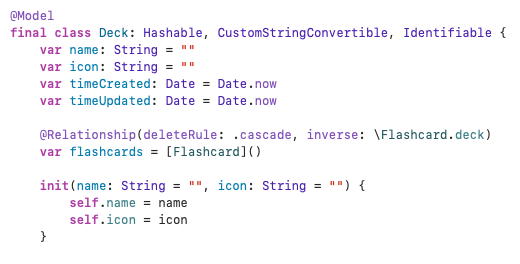
\includegraphics[width=0.7\linewidth]{img/swiftdata1.png}
    \caption{Fragment klasy Deck}
    \label{fig:swiftdata1}
\end{figure}

Definicje modeli znajdują się w plikach \texttt{Flashcard.swift} oraz \texttt{Deck.swift}. W pierwszym z nich przechowywany jest obiekt reprezentujący model fiszki w bazie danych, wraz z zestawem metod go modyfikujących. Dodatkowo znajduje się tam struct \texttt{KnowledgeData} wraz z enumem \texttt{KnowledgeLevel}, które razem reprezentują poziom wiedzy użytkownika dla danej fiszki: niski, średni, albo wysoki. Metody modyfikujące model fiszki pozwalają na zmianę załączonych zdjęć oraz wiedzy o fiszce, a także aktualizowanie informacji o ostatnich zmianach w zestawie. Klasa \texttt{Flashcard} zawiera w sobie również getter koloru reprezentujący aktualną wiedzę fiszki, co  wykorzystywane jest w widoku głównym. Modyfikacja tekstu przedniego oraz tylnego jest dokonywana poprzez przekazywanie \texttt{Binding} do zmiennej widokowi edytora tekstu.


\begin{figure}[H]
    \centering
    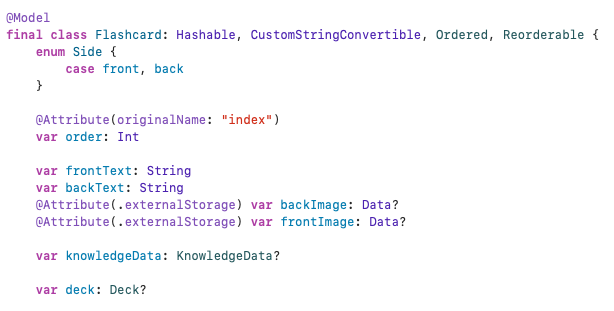
\includegraphics[width=0.7\linewidth]{img/swiftdata2.png}
    \caption{Fragment klasy Flashcard}
    \label{fig:swiftdata2}
\end{figure}


W pliku \texttt{Deck.swift} znajduje się obiekt reprezentujący model zestawu fiszek, który jako swoje metody zawiera możliwości dodawania, usuwania oraz zmieniania kolejności fiszek. Zawarta jest tutaj również metoda nakładająca na zestaw fiszek efekt zaniku wiedzy wraz z upływem czasu. Efekt nakładany jest podczas otwierania danego zestawu w trybie nauki. Kolejną z metod zlokalizowanych w pliku \texttt{Deck.swift} jest sortowanie listy fiszek. Metoda nie działa w sposób kompletnie losowy --- algorytm najpierw dzieli wszystkie fiszki na cztery sekcje w zależności od poziomu nauczenia, lub jego braku. W każdej z czterech kategorii odbywa się losowanie kolejności a następnie wszystkie fiszki łączone są z powrotem w jedną listę, dzięki temu fiszki słabo pamiętane przez użytkownika znajdują się na początku trybu nauczania. Inną ważną metodą w tym pliku zajmuje się obliczaniem procentu wiedzy w danym zestawie fiszek, czyli średniej ważonej z danych o wiedzy każdej fiszki. Obiekt \texttt{Deck} zawiera także statyczne metody służące do dodawania i usuwania zestawów fiszek. 

W folderze \texttt{SwiftData} znajdują się także pliki \texttt{DataModel.swift} oraz \texttt{PreviewSampleData.swift}. Pierwszy z nich definiuje globalny obiekt \texttt{DataModel} będący singletonem, który przechowuje \texttt{ModelContainer}, czyli obiekt zarządzającym modelami bazy danych \texttt{SwiftData}. Drugi plik definiuje modyfikator podglądu widoków, aby ułatwić wyświetlanie danych z modeli \texttt{SwiftData} w widokach.

\begin{figure}[H]
    \centering
    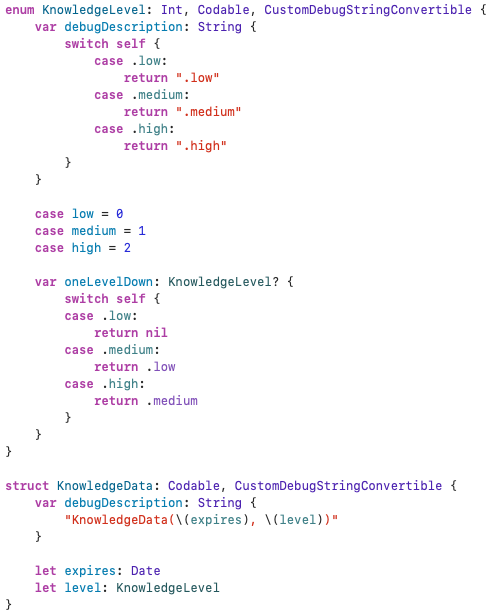
\includegraphics[width=0.7\linewidth]{img/swiftdata3.png}
    \caption{Enum oraz struct pozwalające na zapisywanie stanu wiedzy}
    \label{fig:swiftdata3}
\end{figure}

\section{Plik \texttt{FishkyApp.swift}}

\texttt{FishkyApp.swift} to plik startowy dla całej aplikacji, który definiuje widok bazowy. Ten widok z kolei tworzy zmienną zawierającą \texttt{DataModel}, oraz wywołuje widok główny.

\section{Folder \texttt{Views}}

W tym folderze umieszczone są wszystkie widoki SwiftUI. Widoki zostały podzielone na odpowiednie podfoldery w zależności od tego w jakim ekranie są wykorzystywane. Widoki uniwersalne, czyli mające możliwość użycia w wielu miejscach, zostały umieszczone w folderze o nazwie \texttt{Support}.

\section{Folder \texttt{Views/Home}}

Ten folder reprezentuje widok główny aplikacji. Znajdują się w nim trzy pliki reprezentujące etapy ciągu wywołań na tym ekranie. Plik \texttt{ContentView.swift} jest pierwszym z etapów --- znajduje się w nim  \texttt{NavigationSplitView}, który na większych ekranach będzie tworzył widok podzielony na dwie sekcje: listę elementów oraz widok szczegółów zaznaczonego elementu. Na mniejszych ekranach natomiast będzie wyświetlał samą listę elementów, przy czym kliknięcie na jeden z nich wywoła przejście do jego ekranu szczegółów. Tym ekranem zajmują się widoki w folderze \texttt{Views/Deck}. Widok listy zestawów fiszek znajduje się w pliku \texttt{DeckListView.swift} wywoływanym w \texttt{ContentView.swift}.


\begin{figure}[H]
    \centering
    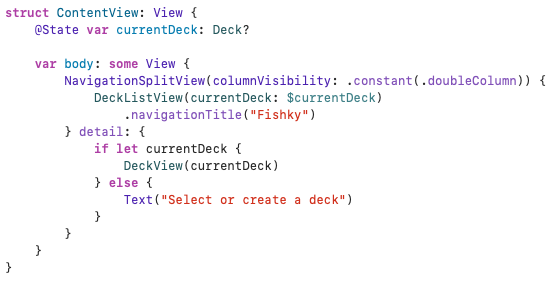
\includegraphics[width=0.7\linewidth]{img/home1.png}
    \caption{Widok ContentView}
    \label{fig:home1}
\end{figure}


Wewnątrz niego znajduje się kod pobierający listę zestawów fiszek z bazy danych, używając makra \texttt{@Query}, a także funkcjonalność dodawania i usuwania ich. Za pomocą operatora \texttt{.toolbar} pasek narzędzi wypełniany jest dwoma przyciskami: pierwszy przełączający tryb edycji oraz drugi, z ikonką plusa, tworzący nowy zestaw fiszek. Znajduje się tutaj także logika gestów przesunięcia fiszki w celu jej usunięcia. 

Część wizualna każdego z elementów jest zamieszczona w pliku \texttt{DeckListItem.swift}. Wyświetla on widok \texttt{NavigationLink}, czyli widok elementu używanego w celu przechodzenia do innej strony, a w nim tytuł zestawu fiszek wraz z procentem wiedzy. 

\section{Folder \texttt{Views/Deck}}

W tym folderze znajdują się wszystkie pliki związane z widokiem zestawu fiszek. Bazowym widokiem jest \texttt{DeckView} z pliku \texttt{DeckView.swift}. Zarządza on elementami, takimi jak tytuł zestawu, guziki dodawania nowej fiszki, guziki włączenia trybu nauki, oraz dodatkowymi elementami konfiguracyjnymi.

Większa część logiki zawarta została w pliku \texttt{FlashcardListView.swift}. Ze względu na to widok ten został rozdzielony na dwie części: część wyświetlającą i część zarządzającą logiką widoku. Do obiektu zarządzającego logiką zostało wykorzystane makro \texttt{@Observable}, które umożliwia widokom SwiftUI monitorowanie zmian obiektu i aktualizowanie widoku po ich dokonaniu. Funkcjonalności zawarte w tym obiekcie to możliwość zmiany kolejności oraz zaznaczenia fiszek w danym momencie. Część wyświetlająca w tym pliku ma za zadanie pokazywać widoki \texttt{AdaptiveList} oraz \texttt{ReorderableForEach}, które są zdefiniowane w innym folderze. Zapewniają one funkcjonalność listy, która dostosowuje się do wielkości ekranu oraz możliwość zmiany kolejności elementów. Wewnątrz listy przechodzącej po każdej z fiszek w danym zestawie wyświetlany zostaje kafelek edycji lub kafelek podglądu fiszki w zależności od stanu trybu edycji. W pierwszym wypadku tryb edycji jest wyłączony a w drugi włączony. Nie brzmi to intuicyjnie --- dlaczego kafelek edycji pojawia się, gdy tryb jest wyłączony? Uzasadnieniem jest fakt, iż podczas przenoszenia fiszki w liście tworzyły się niechciane błędy powodujące wejście wewnętrznego ID danego elementu do jego pola tekstowego. Rozwiązaniem problemu okazała się restrykcja opcji zmiany kolejności tylko do trybu edycji, co pasuje do wzorców znanych w systemie iOS. Dodatkowo podczas zmiany kafelka edycji w kafelek podglądu zaimplementowana została animacja zapewniająca płynne przejście.


\begin{figure}[H]
    \centering
    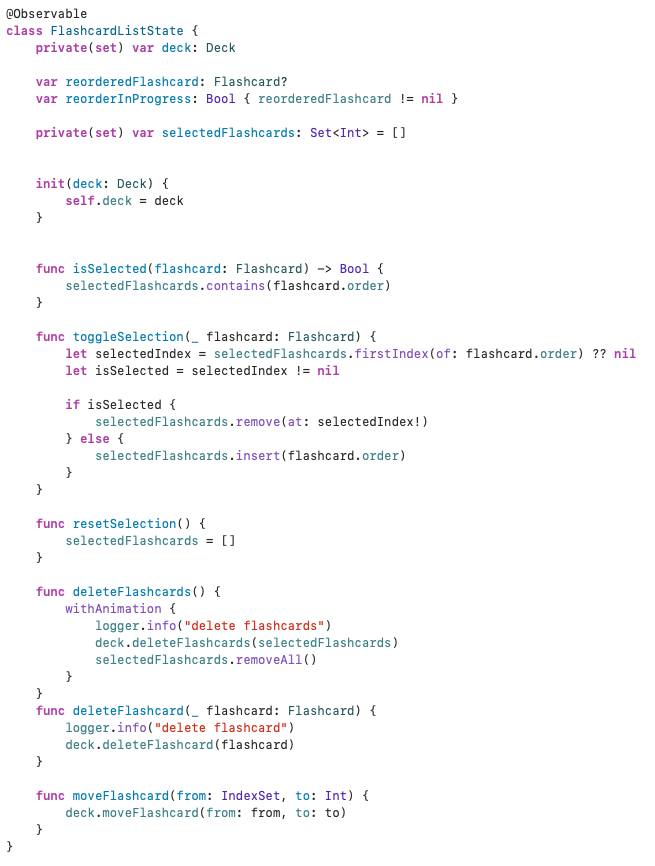
\includegraphics[width=0.7\linewidth]{img/flashcardliststate1.png}
    \caption{Obiekt stanu w pliku FlashcardListView.swift}
    \label{fig:flashcardliststate1}
\end{figure}


Kafelek edycji zawarty jest w pliku \texttt{FlashcardEditTile.swift}. Posiada on dwa pola tekstowe oddzielone linią przerywaną --- pod każdym z nich są załączone zdjęcia lub przyciski ich dodawania. Większość tego widoku zawarta jest w iinnych plikach aplikacji. Sekcja ciała widoku jest złożona z pionowej listy elementów otoczonej szarą ramką , która składa się z edytora tekstu z pliku znajdującego się w folderze \texttt{Support}. Kolejnym jego elementem jest widok \texttt{FlashcardPickerOrImage} z pliku \texttt{FlashcardImage.swift}, niżej znajduje się linia przerywana pliku, widok \texttt{FlashcardPickerOrImage} oraz edytor tekstu.

Widok zajmujący się wyświetlaniem zdjęć w pliku \texttt{FlashcardImage.swift} zawiera także funkcjonalność wyświetlaniem guzika dodawania zdjęcia. Taka struktura została wybrana, aby każdy etap zarządzania zdjęciami był zmieszczony w tym widoku, a do bazy danych zapisywane zostały tylko ostateczne zdjęcia w formacie binarnym. W tym pliku stan widoku został wydzielony do osobnego obiektu i tak samo jak poprzednio jest on definiowany przy pomocy makro \texttt{@Observable}. Ten stan przechowuje w sobie referencję do obiektu danej fiszki w bazie danych, informację o stronie fiszki (przód czy tył) w formie enum oraz obiekt \texttt{PhotosPickerItem}. Obiekt ten jest zwracany przez wbudowany widok \texttt{PhotosPicker} i przechowuje w sobie tymczasowo wybrane zdjęcie. W pliku \texttt{FlashcardImage.swift} obecne są również gettery upraszczające logikę samego widoku: jeden zwraca odpowiednie dane binarne zdjęcia w zależności od strony fiszki, drugi konwertuje dane binarne na reprezentację możliwą do użycia w interfejsie użytkownika. Znajdują się w nim także dwie metody do zarządzania zdjęciami w pamięci. Pierwsza z nich usuwa zdjęcia z fiszki, natomiast druga dodaje zdjęcia zamieniając je na format binarny. Zamiana ta zamknięta jest w bloku \texttt{Task}, ponieważ operacje związane z konwersją formatu zdjęcia na binarny są asynchroniczne. Wymagają więc wyodrębnienia jako osobne ,,zadanie''. W sekcji wyświetlającej ten widok znajduje się instrukcja warunkowa, która zajmuje się wyświetlaniem dostępnego zdjęcia lub, w razie jego braku, wyświetlaniem przycisku jego dodawania.

Pozostałe pliki w tym folderze to \texttt{NewFlashcardButton.swift}, gdzie znajduje się definicja guzika dodawania nowych fiszek, oraz \texttt{FlashcardPreviewTile.swift}, który definiuje podgląd \texttt{FlashcardEditTile} z guzikami o szarej barwie. Kolor ten został użyty w celu podkreślenia brak możliwości interakcji.

\section{Folder \texttt{Views/Study}}

Po kliknięciu guzika włączania trybu nauki otwiera się pełnoekranowy widok nauki. Zarządza nim folder \texttt{Views/Study}. Cały widok jest podzielony na trzy części: lista fiszek wyświetlana w pliku \texttt{FullscreenStudyView.swift}, widok pojedynczej fiszki w pliku \texttt{FlashcardStudyView.swift}, oraz guziki do zaznaczania znajomości materiału naukowego w pliku \texttt{KnowledgeButtons.swift}.

W pliku \texttt{FullscreenStudyView.swift} widok jest podzielony na obiekt stanu i obiekt wyglądu. Obiekt stanu posiada pięć zmiennych: odnośnik do zestawu fiszek w bazie danych, listę fiszek dla danej sesji, listę zapisującą stan odwrócenia fiszek, listę zapisującą widoczność przycisków wiedzy przy fiszkach, oraz zmienną oznaczająca oczekiwanie na przygotowanie wszystkich innych zmiennych. Ostatnia z nich zmienia się podczas wywoływania funkcji \texttt{initialize}, która bierze z bazy danych fiszki i miesza je bazując na stanie wiedzy. Oprócz tego w obiekcie stanu znajdują się również dwie metody. Jedna z nich zajmuje się animacją obracania danej fiszki, przy czym odpowiednio opóźnia animację pojawiania się guzików, aby zapewnić lepsze zgranie elementów interfejsu. Druga metoda zwraca widoczność guzików dla odpowiedniego indeksu elementu. W sekcji wyglądu widoku wyświetlany jest widok przesuwalny (\texttt{ScrollView}). Nałożone na niego odpowiednie modyfikatory zapewniają, iż przewijanie odbywa się po jednej fiszce naraz. Pod-widokami widoku przesuwalnego  są widoki nauki fiszki, których częścią są widoki przycisków wiedzy. Nałożone na nie zostały specjalne modyfikatory zapewniające wypełnienie całej dostępnej na ekranie przestrzeni. Dodatkowo na samym jego końcu umieszczony jest widok końca nauki przypominający fiszkę, który zawiera w sobie przycisk do zakończenia trybu nauki.


\begin{figure}[H]
    \centering
    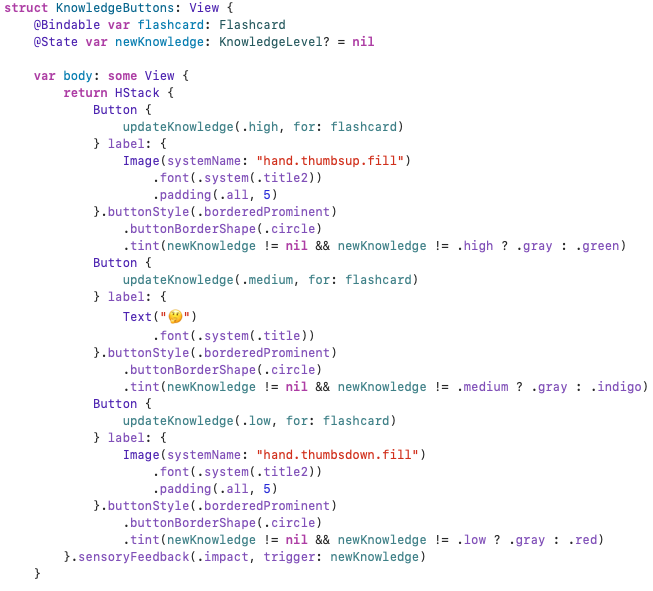
\includegraphics[width=0.7\linewidth]{img/knowledgebuttons1.png}
    \caption{Fragment widoku KnowledgeButtons}
    \label{fig:knowledgebuttons1}
\end{figure}


Widok nauki fiszki znajduje się w pliku \texttt{FlashcardStudyView.swift}. Zawiera on w sobie dwa widoki: widok pojedynczej karty, oraz widok pełnej fiszki. Widok karty dostaje jako argumenty treść danej strony fiszki, dane ewentualnego zdjęcia, oraz stopień obrócenia. Na kartę zostaje nałożony efekt obrotu trójwymiarowego zgodny z podanymi stopniami. Sama karta składa się z zaokrąglonego prostokąta z nałożonym na niego tekstem i ewentualnym zdjęciem. Dodatkowo nałożone zostały na nią modyfikatory wyglądu --- kolor biały, proporcje 2:3 oraz cień. Wewnątrz widoku pełnej fiszki utrzymywany jest stan rotacji oraz stopień obrotu zarówno przedniej jak i tylnej strony. Obie strony karty reprezentowane są poprzez oddzielne nałożone na siebie widoki widoczne tylko, gdy ich stopień obrócenia na to pozwala. Po kliknięciu w kartę najpierw wywołuje się animacja obrotu według jej osi pionowej. To sprawia, że karta przestaje być widoczna na ekranie --- prawie jakby się ,,schowała''. Po zakończeniu obrotu wywoływany jest kolejny obrót, tym razem karty o przeciwnej stronie fiszki od obecnie niewidocznej, co sprawia, iż pojawia się ona na ekranie. Płynność obu animacji daje złudzenie istnienia jednej karty wypełnionej treścią po obu stronach. Cały system obrotu kart bazowany jest na artykule Jonathana Rasmussona \cite{card_flip} udostępnionym na platformie GitHub.



Przyciski zawarte w pliku \texttt{KnowledgeButtons.swift} są złożone z trzech guzików w kształcie koła, z kolorami zależnymi od stanu guzika --- wybrany zachowuje swój kolor, podczas gdy reszta staje się szara.

\section{Folder \texttt{Views/Support/}}

Widok edytora tekstu zawarty jest w pliku \texttt{TextEditorView.swift}. Biblioteka  \texttt{SwiftUI} posiada wbudowany edytor tekstu \texttt{TextEditor}, jednak nie mógł on być zastosowany samodzielnie w tej aplikacji --- powodował on błędy układu struktury strony. Przykładem mogą być dwa pola tekstowe reprezentujące treści po obu stronach fiszki. Podczas zmiany wysokości jednego pola drugie z nich automatycznie dostosowywało się do takiej samej wysokości. Efektem tego był mało estetyczny wygląd fiszek. Przy rozwiązaniu tego problemu pomocny okazał się użytkownik portalu Stack Overflow \cite{so_texteditor}. Zaproponowane rozwiązanie zakładało nałożenie na siebie \texttt{TextEditor}, niewidzialnego widoku normalnego tekstu oraz \texttt{GeometryReader}, którego zadaniem jest odczytywanie i egzekwowanie wysokości docelowej widoku tekstu. 

Urządzenia mają różne rozmiary --- na mniejszych z nich ułożenie elementów w listę może być bardziej sensowne, a na innych w siatkę. Do tego właśnie celu został utworzony widok zawarty w pliku \texttt{AdaptiveList.swift}. Widok ten ma możliwość dostać dowolną listę widoków i na podstawie klasy rozmiaru urządzenia wyświetli elementy w pasującym do niej układzie.

W pliku \texttt{ReorderableForEach.swift} znajduje się widok umożliwiający zmianę kolejności elementów. Jest on dość mocno inspirowany artykułem Daniela Saidi ,,Enabling drag reordering in lazy SwiftUI grids and stacks''\cite{drag_reordering}. Widok wykorzystuje modyfikatory \texttt{onDrag} oraz \texttt{onDrop}, aby wykrywać podnoszenie, upuszczanie, oraz zmianę pozycji elementów przenoszonych. Dodatkowo zawarty w pliku został rownież delegat upuszczania i przenoszenia elementu, które z wykorzystaniem wyżej wspomnianych modyfikatorów zarządzają stanem przenoszenia.


\chapter*{Podsumowanie}

Celem pracy było stworzenie minimalistycznej aplikacji do nauki za pomocą fiszek. Rezultatem jest aplikacja na system iOS spełniająca wszystkie określone na początku pracy wymogi. Pozwala na zapełnianie tekstem obu stron fiszek, a także dodawanie zdjęć.

Aplikacja wyróżnia się na tle konkurencji minimalistycznym interfejsem bez zbędnej funkcjonalności zaciemniającej jej cel dydaktyczny. Intuicyjny układ zapewnia prostotę w użytku, a użytkownik jest na bieżąco informowany o jego postępach w nauce. Ponadto tryb nauczania z inteligentnym układaniem fiszek dostosowuje się do aktualnego poziomu wiedzy użytkownika w celu optymalizowania efektów nauki. 

Aplikacja w obecnej wersji stanowi solidną podstawę do dalszego rozwoju. W perspektywie planowanych modyfikacji jest zapewnienie użytkownikowi możliwości robienia zdjęć wewnątrz aplikacji oraz przycinania ich. Dzięki dużym możliwością biblioteki SwiftUI aplikacja może zostać zaadaptowana do działania na komputerach z systemem macOS. Następnym krokiem mogłaby być też adaptacja na kolejne platformy ekosystemu Apple, aby możliwość nauki była dostępna na systemach watchOS oraz tvOS. W przypadku aplikacji działającej na tylu platformach potrzebna, by była także funkcjonalność synchronizacji aplikacji z chmurą iCloud, co jest jedną z funkcjonalności wbudowanych w bibliotekę SwiftData.
Dalszy rozwój aplikacji jest możliwy, aktualny stan jest satysfakcjonujący i spełnia wszystkie założone oczekiwania.





\bibliographystyle{plain}
\bibliography{mgr}

\end{document} 